% Copyright (c) 2020 Carl Martin Ludvig Sinander.

% This program is free software: you can redistribute it and/or modify
% it under the terms of the GNU General Public License as published by
% the Free Software Foundation, either version 3 of the License, or
% (at your option) any later version.

% This program is distributed in the hope that it will be useful,
% but WITHOUT ANY WARRANTY; without even the implied warranty of
% MERCHANTABILITY or FITNESS FOR A PARTICULAR PURPOSE. See the
% GNU General Public License for more details.

% You should have received a copy of the GNU General Public License
% along with this program. If not, see <https://www.gnu.org/licenses/>.

%                                   _     _      
%    _ __  _ __ ___  __ _ _ __ ___ | |__ | | ___ 
%   | '_ \| '__/ _ \/ _` | '_ ` _ \| '_ \| |/ _ \
%   | |_) | | |  __/ (_| | | | | | | |_) | |  __/
%   | .__/|_|  \___|\__,_|_| |_| |_|_.__/|_|\___|
%   |_|                                          


%%% bug catcher
\RequirePackage[l2tabu,orthodox]{nag}

%%% document class
\documentclass[11pt,letterpaper,reqno,oneside]{article}

%%% settings
\input{preamble.tex}

%%% bibliography
\addbibresource{bibl.bib}

%%% externalise TikZ drawings
% \usetikzlibrary{external}
% \tikzexternalize



%______________________________________________________________________________




%    _____ _ _   _      
%   |_   _(_) |_| | ___ 
%     | | | | __| |/ _ \
%     | | | | |_| |  __/
%     |_| |_|\__|_|\___|


\title{\scshape Topics in game theory \\
	\vspace{0.5em}
	\large \scshape Taught by Eran Shmaya \\
	\large \scshape Northwestern University, fall 2016
	}

\author{Ludvig Sinander \\ Northwestern University}

\date{\small This version: 12 June 2025}

\makeatletter
	\AtBeginDocument{ \hypersetup{ 
		pdftitle = {Topics in game theory}, 
		pdfauthor = {Ludvig Sinander} 
		} }
\makeatother



%______________________________________________________________________________




%    ____                                        _   
%   |  _ \  ___   ___ _   _ _ __ ___   ___ _ __ | |_ 
%   | | | |/ _ \ / __| | | | '_ ` _ \ / _ \ '_ \| __|
%   | |_| | (_) | (__| |_| | | | | | |  __/ | | | |_ 
%   |____/ \___/ \___|\__,_|_| |_| |_|\___|_| |_|\__|


\begin{document}

\maketitle


\noindent
These notes are based on a theory course for second-year PhD students taught by Eran Shmaya at Northwestern in fall 2016. The topics are mechanism/auction design, supermodular games, and learning.\\

\noindent
I thank Eran for teaching a great class and for agreeing to let me share these notes, and Matteo Escudé, Egor Starkov, Ben Vatter, Haihan Yu, Klavdia Zemlianova and Andrey Zhukov for reporting errors.



\pagebreak
\hspace{1pt}\vfill
\noindent
Copyright \copyright{} 2020 Carl Martin Ludvig Sinander.

\begin{quotation}
\noindent
Permission is granted to copy, distribute and/or modify this document under the terms of the \href{https://www.gnu.org/licenses/fdl}{GNU Free Documentation License}, Version 1.3 or any later version published by the Free Software Foundation; with no Invariant Sections, no Front-Cover Texts, and no Back-Cover Texts. A copy of the license is included in the section entitled `GNU
Free Documentation License'.
\end{quotation}

\noindent
This is a `copyleft' licence.
Visit \href{https://www.gnu.org/licenses/copyleft}{gnu.org/licenses/copyleft} to learn more.



%%%%%%%%%%%%%%%%%%%
%%%%%%%%%%%%%%%%%%%
% Table of contents
\pagebreak
\microtypesetup{protrusion=false}
\tableofcontents
\microtypesetup{protrusion=true}
%%%%%%%%%%%%%%%%%%%
%%%%%%%%%%%%%%%%%%%



\pagebreak
%%%%%%%%%%%%%%%%%%%%%%%%%%
%%%%%%%%%%%%%%%%%%%%%%%%%%
\section{Mechanism design}
\label{sec:mech_desi}
%%%%%%%%%%%%%%%%%%%%%%%%%%
%%%%%%%%%%%%%%%%%%%%%%%%%%

\emph{This section doesn't follow any book, but the treatment shares features with \textcite{Vohra2011}.}

We begin with mechanism design in a simple environment: a single indivisible object has to be allocated to (at most) one of $n$ agents whose valuations for it are independently distributed private information. We will sweat this framework pretty hard, and then examine what can be said for more general type spaces and for the case of correlated values.

As a simple motivation, consider a principal allocating a single, indivisible object between two agents. An agent's $i$'s type is her valuation $t_i \in \mathcal{T}_i \subseteq \R$ for the object. $t_i$ is unknown to the principal, who views it as a random variable $T_i$ distributed with CDF $F_i$. Further, the principal and agents believe that $T_1$ and $T_2$ are distributed independently. Type $t_i$ of agent $i$ derives zero value from not obtaining the object, value $t_i$ from obtaining the object, and maximises her expected utility.

For concreteness, let $T_i \sim \mathcal{U}[0,1]$. One way to allocate the object is using an auction, e.g. a first-price sealed-bid auction or a second-price sealed-bid auction. As we'll see, these two auctions raise the same revenue, and adding a reserve price may increase revenue further.

In the second-price auction, it's weakly dominant for each player to bid her value, so that `truthful' bidding constitutes a Bayes--Nash equilibrium. Expected revenue is then $\E\left( T_1 \meet T_2 \right) = 1/3$.

In the first-price auction, there is a Nash equilibrium in which both players bid $\alpha(t_i) = t_i/2$ for each $t_i \in [0,1]$. To verify this, suppose that player $j$ plays $\alpha$. If type $t_i$ of player $i$ bids $a_i$, her payoff is
%
\begin{equation*}
	\PP( \alpha(T_j) < a_i ) \cdot (t_i-a_i)
	= \PP( T_j < 2 a_i ) \cdot (t_i-a_i) = 2 a_i (t_i-a_i) ,
\end{equation*}
%
which is maximised at $a_i=t_i/2$. Revenue is then $\E\left( T_1 \join T_2 \right) / 2 = 1/3$, the same.

In an auction with a reserve price $\underline{b}$, the object is not allocated to either player if they both bid below $\underline{b}$. In general, this means that the object remains unallocated with positive probability. We shall see that the revenue-maximising way of selling the object is to run an auction with a strictly positive reserve price.



\pagebreak
%%%%%%%%%%%%%%%%%%%%%%%%%%%%%%%%%%%%%%%%%%%%%%%%
\subsection{Single agent, one-dimensional types}
\label{sec:mech_desi:single_agent_one_dimension}
%%%%%%%%%%%%%%%%%%%%%%%%%%%%%%%%%%%%%%%%%%%%%%%%


%%%%%%%%%%%%%%%%%%%%%%%%%%%%%%%%%%%%%%%%%%%%%%%%%%%%%%%%%%%%%%%%
\subsubsection{Convex analysis on one-dimensional domains}
\label{sec:mech_desi:single_agent_one_dimension:convex_analysis}

We're going to need some tools from convex analysis. We'll provide results for convex functions defined on intervals of $\R$; extensions to multidimensional domains will be covered in \cref{sec:mech_desi:single_agent_multiple_dimensions:convex_analysis_multi}. Proofs, details and related results can be found in \textcite{Rockafellar1970}.

\begin{definition}
	%
	$f : [a,b] \to \R$ is convex iff for any $x,x' \in [a,b]$ and $\lambda \in [0,1]$,
	%
	\begin{equation*}
		f( \lambda x + (1-\lambda) x' ) \leq \lambda f(x) + (1-\lambda) f(x') .
	\end{equation*}
	%
\end{definition}


\begin{proposition}
	%
	\label{proposition:convex_preserved_1d}
	%
	Let $\{ f_\alpha \}$ be a family of convex functions $[a,b] \to \R$. Define $f : [a,b] \to \R$ by $f(x) \coloneqq \sup_\alpha f_\alpha(x)$ $\forall x \in [a,b]$. Then $f$ is convex.
	%
\end{proposition}
%
% Since affine functions are convex, a corollary is that the pointwise maximum of affine functions is convex. There's also a converse: every convex function can be written as the maximum of affine functions (constructed from the subdifferential; see below).


For $f : [a,b] \to \R$ convex, $x^\star \in \R$ is a subgradient of $f$ at $x \in [a,b]$ iff
%
\begin{equation*}
	f(x') \geq f(x) + x^\star (x'-x)
	\quad\forall x' \in [a,b] .
\end{equation*}
%
This means precisely that the affine map $x' \mapsto f(x) + x^\star (x'-x)$ is everywhere weakly below $f$, and equal to $f$ at $x$. The subdifferential of a convex function $f : [a,b] \to \R$ is the correspondence $\partial f : [a,b] \Rightarrow \R$ such that $\partial f(x)$ is the set of all subgradients of $f$ at $x$. For $f,g \in \R^{[a,b]}$, we write `$g \in \partial f$' as shorthand for `$g(x) \in \partial f(x)$ for each $x \in [a,b]$'.

\begin{proposition}
	%
	\label{proposition:convex_subgrad_1d}
	%
	Let $f : [a,b] \to \R$ be convex. Then
	%
	\begin{enumerate}

		\item $\partial f(x)$ is nonempty, compact and convex for every $x \in [a,b]$.

		\item $f'_+(x)$ exists at every $x \in [a,b)$, and $f'_-(x)$ exists at every $x \in (a,b]$.%
			\footnote{These are, respectively, the right- and left-hand derivatives of $f$ at $x$.}

		\item $\partial f(x) = \left[ f'_-(x), f'_+(x) \right]$ for every $x \in (a,b)$.

	\end{enumerate}
	%
\end{proposition}


\begin{proposition}
	%
	\label{proposition:convex_properties_1d}
	%
	Let $f : [a,b] \to \R$ be convex. Then
	%
	\begin{enumerate}

		\item $f$ is continuous.

		\item $f$ is differentiable outside a countable subset of $(a,b)$.

		\item If $a < x < x' < b$ then $f'_+(x) \leq f'_-(x')$. (So $\partial f$ is monotone.)

	\end{enumerate}
	%
\end{proposition}

\begin{remark}
	%
	(2) does not generalise to the case in which the domain of $f$ is a compact and convex subset of $\R^m$ for $m \geq 2$. It remains true that a convex function is differentiable a.e.
	%
\end{remark}

A very useful property of convex functions is that they admit a fundamental theorem of calculus. A proof can be found in \textcite[][p. 232]{Rockafellar1970}.
%
\begin{theorem}[convex FToC]
	%
	\label{theorem:convex_FTC_1d}
	%
	Let $f,g \in \R^{[a,b]}$. The following are equivalent:
	%
	\begin{enumerate}

		\item $f$ is convex, and $g \in \partial f$.

		\item $g$ is increasing, and $f(x) = f(a) + \int_a^x g$ for each $x \in [a,b]$.%
			\footnote{That's a Riemann integral. Monotone functions are always Riemann-integrable.}

	\end{enumerate}
	%
\end{theorem}


\begin{corollary}
	%
	\label{corollary:convex_FTC_1d}
	%
	Let $g : [a,b] \to \R$.
	%
	\begin{enumerate}

		\item $g$ is increasing iff $g \in \partial f$ for some convex $f : [a,b] \to \R$.

		\item If $g \in \partial f$ for $f : [a,b] \to \R$ convex, then
		%
		\begin{equation*}
			f(x) - f(x') = \int_{x'}^x g
			\quad\text{for every $x,x' \in [a,b]$} .
		\end{equation*}		

	\end{enumerate}
	%
\end{corollary}

\begin{proof}
	%
	If there is $f$ convex such that $g \in \partial f$, then $g$ is increasing by \Cref{theorem:convex_FTC_1d}. If $g$ is increasing, define $f(x) \coloneqq \int_a^x g$; then $f$ is convex and $g \in \partial f$ by \Cref{theorem:convex_FTC_1d}. Part (2) is immediate from \Cref{theorem:convex_FTC_1d}.
	%
\end{proof}

\Cref{corollary:convex_FTC_1d} is certainly not as neat as the full FToC. I present it because it is sufficient for our purposes and because unlike the FToC, it generalises directly to the multidimensional case (see \cref{sec:mech_desi:single_agent_multiple_dimensions:convex_analysis_multi}).



%%%%%%%%%%%%%%%%%%%%%%%%%%%%%%%%%%%%%%%%%%%%%%%%%%%%%%%%%%
\subsubsection{Environment}
\label{sec:mech_desi:single_agent_one_dimension:environment}

Begin with the case of a single buyer. The buyer has type $t \in \mathcal{T}$, where $\mathcal{T} = \left[ \underline{t}, \bar{t} \right] \subseteq \R$. Her type is unknown to the principal, who views it as a random variable $T$ distributed with CDF $F$. If the agent is of type $t$ and pays transfer $p$ to the principal, she earns utility $t-p$ if she gets the object and $-p$ if she does not. (So she is risk-neutral and has a type-independent outside option.) She maximises expected utility.

A direct mechanism in this setting is a pair of functions $g : \mathcal{T} \to [0,1]$ and $p : \mathcal{T} \to \R$ such that if the agent reports her type as $t$, she wins the object with probability $g(t)$ and pays transfer $p(t)$. (Note that she pays the transfer $p(t)$ regardless of whether she gets the object.) So an agent of type $t$ who reports her type as $t'$ earns a payoff of $g(t') t - p(t')$. We call $g$ the allocation rule and $p$ the transfer rule.

\begin{definition}
	%
	Let $(g,p)$ be a direct mechanism.
	%
	\begin{enumerate}

		\item $(g,p)$ is incentive-compatible (IC) iff
		%
		\begin{equation*}
			g(t) t - p(t) \geq g(t') t - p(t')
			\quad\text{for every $t,t' \in \mathcal{T}$} .
		\end{equation*}

		\item $(g,p)$ is individually rational (IR) iff $g(t) t - p(t) \geq 0$ for every $t \in \mathcal{T}$.

		\item $g$ is implementable iff there is a $p : \mathcal{T} \to \R$ s.t. $(g,p)$ is IC.

	\end{enumerate}
	%
\end{definition}

As usual, a revelation principle applies, so that we can restrict attention to direct mechanisms that satisfy IC and IR. We'd like to characterise the set of IC and IR direct mechanisms, and then to find the mechanism in that set which maximises expected revenue $\E(p(T))$ for the principal. %(Preview: the revenue-maximising mechanism will be a posted price, with the price determined by $F$. This is a one-agent \textcite{Myerson1981} auction with a reserve price.)



%%%%%%%%%%%%%%%%%%%%%%%%%%%%%%%%%%%%%%%%%%%%%%%%%%%%%%%%%%%%%%%%%%%%
\subsubsection{Characterisation of IC}
\label{sec:mech_desi:single_agent_one_dimension:IC_characterisation}

In this section, we give two results that sharply characterise the set of IC direct mechanisms. The Spence--Mirrlees theorem shows that an allocation rule $g$ is implementable iff it is increasing. The Mirrlees envelope theorem shows that, up to a constant, any IC mechanism implementing $g$ must have the same payments and payoffs.

The key to proving these results is to translate implementability into a statement about the subdifferential of a convex functions; once that's done, the fundamental theorem of calculus for convex functions (\Cref{theorem:convex_FTC_1d}) does the rest.
%
\begin{lemma}
	%
	\label{lemma:implementable_subdifferential_1d}
	%
	$g : \mathcal{T} \to [0,1]$ is implementable iff $g \in \partial \phi$ for some convex $\phi : \mathcal{T} \to \R$.
	%
\end{lemma}

\begin{proof}
	%
	Suppose that $g$ is implementable. Then there is $p : \mathcal{T} \to \R$ such that $(g,p)$ is IC. Define $\phi$ from $g$ and $p$ as 
	%
	\begin{equation*}
		\phi(t) \coloneqq \max_{t' \in \mathcal{T}} \left[ g(t') t - p(t') \right]
		\quad \text{for each $t \in \mathcal{T}$} .
	\end{equation*}
	%
	Since $\phi$ is the pointwise maximum of convex functions, it is convex. Moreover, for every $t,t' \in \mathcal{T}$,
	%
	\begin{align*}
		\phi(t')
		\geq{}& g(t) t' - p(t)
		\\
		={}& [ g(t) t - p(t) ] + g(t) (t'-t)
		\\
		={}& \phi(t) + g(t) (t'-t) ,
	\end{align*}
	%
	where the first inequality used the definition of $\phi$, and the second used IC. So $g \in \partial \phi$ for $\phi$ convex.

	Now suppose that $g \in \partial \phi$ for some $\phi : \mathcal{T} \to \R$ convex. Define $p : \mathcal{T} \to \R$ from $g$ and $\phi$ by
	%
	\begin{equation*}
		p(t) \coloneqq g(t) t - \phi(t)
		\quad\text{for each $t \in \mathcal{T}$} .
	\end{equation*}
	%
	Then for every $t,t' \in \mathcal{T}$,
	%
	\begin{align*}
		g(t) t - p(t) 
		={}& \phi(t)
		\\
		\geq{}& \phi(t') + g(t') (t-t')
		\\
		={}& [ g(t') t' - p(t') ] + g(t') (t-t')
		\\
		={}& g(t') t - p(t') ,
	\end{align*}
	%
	where the first and second equalities used the definition of $p$, and the inequality used $g(t') \in \partial \phi(t')$. So $(g,p)$ is IC, hence $g$ is implementable.
	%
\end{proof}


Since the subdifferentials of convex functions are precisely the increasing functions, we obtain the following.
%
\begin{theorem}[\textcite{Spence1974}, \textcite{Mirrlees1976}]
	%
	\label{theorem:implementable_monotone_1d}
	%
	$g$ is implementable iff it is increasing.
	%
\end{theorem}

\begin{proof}
	%
	Immediate from \Cref{lemma:implementable_subdifferential_1d} and part (1) of \Cref{corollary:convex_FTC_1d} (p. \pageref{corollary:convex_FTC_1d}).
	%
\end{proof}


The function $\phi$ that we constructed in the first part of the proof of \Cref{lemma:implementable_subdifferential_1d} will continue to be useful: for a mechanism $(g,p)$, let $\phi^{g,p} : \mathcal{T} \to \R$ be given by
%
\begin{equation*}
	\phi^{g,p}(t) \coloneqq \max_{t' \in \mathcal{T}} \left[ g(t') t - p(t') \right]
	\quad \text{for each $t \in \mathcal{T}$} .
\end{equation*}
%
$\phi^{g,p}(t)$ is the payoff that type $t$ gets from the mechanism $(g,p)$. $\phi^{g,p}$ is obviously convex by construction, and we showed in the proof of \Cref{lemma:implementable_subdifferential_1d} that $g \in \partial \phi^{g,p}$ if $(g,p)$ is IC.


Since a convex function is determined up to a constant by its subdifferential, we have the following envelope theorem:
%
\begin{theorem}[\textcite{Mirrlees1971}]
	%
	\label{theorem:IC_envelope_1d}
	%
	If $(g,p)$ is IC then
	%
	\begin{equation*}
		\phi^{g,p}(t) - \phi^{g,p}(t') 
		= \int_{t'}^t g
		\quad\text{for every $t,t' \in \mathcal{T}$} .
	\end{equation*}
	%
\end{theorem}

\begin{proof}
	%
	Immediate from \Cref{lemma:implementable_subdifferential_1d} and part (2) of \Cref{corollary:convex_FTC_1d} (p. \pageref{corollary:convex_FTC_1d}).
	%
\end{proof}


The Mirrlees envelope theorem delivers the familiar payoff and revenue equivalence results:
%
\begin{corollary}[payoff \& revenue equivalence]
	%
	If $(g,p)$ and $(g,p')$ are IC then
	%
	\begin{equation*}
		\phi^{g,p} - \phi^{g,p'} = p'-p = k
	\end{equation*}
	%
	for some $k \in \R$.
	%
\end{corollary}


It's obvious from the Mirrlees envelope theorem that $\phi^{g,p}$ is increasing for any IC $(g,p)$. Hence
%
\begin{corollary}
	%
	If $(g,p)$ is IC, then it is IR iff $\phi^{g,p}(\underline{t}) \geq 0$.
	%
\end{corollary}
%
\noindent It follows that IR imposes no constaints on implementability: if $(g,p)$ is IC but not IR, then $(g,p - \phi^{g,p}(\underline{t}))$ is also IC, and is IR by construction.


\begin{remark}
	%
	It's important for the envelope formula that IC hold on a connected set (in our case an interval $\mathcal{T} = \left[ \underline{t}, \bar{t} \right]$). When there are gaps, our fundamental theorem of calculus is inapplicable, and results such as revenue equivalence may fail.
	%
\end{remark}



%%%%%%%%%%%%%%%%%%%%%%%%%%%%%%%%%%%%%%%%%%%%%%%%%%%%%%%%%%%%%%%%%%%%%%%%%
\subsubsection{Optimal mechanism}
\label{sec:mech_desi:single_agent_one_dimension:revenue-maxing_mech_sing}

By the envelope formula, if $(g,p)$ is IC and IR then type $t$ pays
%
\begin{equation*}
	p(t) = g(t) t - \int_{\underline{t}}^t g
	- \phi^{g,p}\left( \underline{t} \right) ,
\end{equation*}
%
where $\phi^{g,p}\left( \underline{t} \right)$ is any nonnegative number. Clearly revenue is maximised by setting $\phi^{g,p}\left( \underline{t} \right) = 0$, so that
%
\begin{equation}
	\label{eq:optimal_p_form}
	p(t) = g(t) t - \int_{\underline{t}}^t g .
\end{equation}
%
Expected revenue as a function of $g$ alone is then
%
\begin{equation*}
	R(g) 
	\coloneqq \E\left( g(T) T 
	- \int_{\underline{t}}^T g \right)  .
\end{equation*}
%
The principal's problem is to maximise $R(g)$ subject to $g \in \mathcal{M}_1$, where $\mathcal{M}_1$ denotes the set of increasing functions $\mathcal{T} \to [0,1]$.

$R$ is evidently linear:
%
\begin{equation*}
	R( \alpha g + \alpha' g' ) = \alpha R(g) + \alpha' R(g') .
\end{equation*}
%
$\mathcal{M}_1$ is clearly convex; it is also compact in the product topology.%
	\footnote{$[0,1]^\mathcal{T}$ is compact by Tychonoff's theorem, and $\mathcal{M}_1$ is closed in $[0,1]^\mathcal{T}$, hence compact.}
Since we're maximising a linear function on a compact and convex constraint set, the maximum is attained at an extreme point of the constraint set. The extreme points of $\mathcal{M}_1$ are precisely the functions of the form
%
\begin{equation*}
	g = \1_{\left[t^\star,\bar{t}\right]}
	\quad\text{or}\quad
	g = \1_{\left(t^\star,\bar{t}\right]} 
	\quad\text{for some $t^\star \in \mathcal{T}$}.
\end{equation*}

So we've shown that the optimal mechanism is deterministic.%
	\footnote{Not a trivial result. It doesn't hold with multiple objects. It relies heavily on linearity and the one-dimensional structure.}
Further, we've shown that the object is assigned according to a threshold rule. By \eqref{eq:optimal_p_form}, all types below $t^\star$ pay $p(t)=0$, and types above $t^\star$ pay
%
\begin{equation*}
	p(t) 
	= t - \int_{t^\star}^t \dd t' 
	= t^\star .
\end{equation*}
%
So the optimal mechanism is a posted price $t^\star$.

Clearly expected revenue from posting the price $t^\star$ is
%
\begin{equation*}
	\left[ 1 - F\left( t^\star \right) \right] t^\star .
\end{equation*}
%
(Recall that $F$ is the CDF of the agent's type $T$.) The optimal price is the one that maximises this expression. When the CDF $F$ of has a density $f$, the optimal price solves the first-order condition
%
\begin{equation*}
	1 - F\left( t^\star \right) - f\left( t^\star \right) t^\star = 0 .
\end{equation*}



\pagebreak
%%%%%%%%%%%%%%%%%%%%%%%%%%%%%%%%%%%%%%%%%%%%%%%%%%%%%%%%%%%%%%
\subsection{Several agents, one-dimensional independent types}
\label{sec:mech_desi:several_agents_one_dimension}
%%%%%%%%%%%%%%%%%%%%%%%%%%%%%%%%%%%%%%%%%%%%%%%%%%%%%%%%%%%%%%


%%%%%%%%%%%%%%%%%%%%%%%%%%%%%%%%%%%%%%%%%%%%%%%%%%%%%%%%%%%%%%
\subsubsection{Environment}
\label{sec:mech_desi:several_agents_one_dimension:environment}

Now suppose that there are $n$ agents indexed by $i \in \{1,\dots,n\}$. Their types are $t = (t_1,\dots,t_n) \in \prod_{i=1}^n \mathcal{T}_i \eqqcolon \mathcal{T}$, where each $\mathcal{T}_i = \left[ \underline{t}_i, \bar{t}_i \right]$ is an interval of $\R$. The principal views types as independently distributed random variables $\{ T_i \}$ with marginal CDFs $\{ F_i \}$. Preferences are as before.

A direct mechanism is a pair $(g,p)$ of an allocation rule $g : \mathcal{T} \to [0,1]^n$ such that $\sum_{i=1}^n g_i(t) \leq 1$ and a transfer rule $p : \mathcal{T} \to \R^n$.



%%%%%%%%%%%%%%%%%%%%%%%%%%%%%%%%%%%%%%%%%%%%%%%%%%%%%%%%%%%%%%%%%%%%%%%
\subsubsection{Bayesian implementation}
\label{sec:mech_desi:several_agents_one_dimension:BIC_characterisation}

Consider Bayesian implementation: we design a game and assume that agents play a Bayes--Nash equilibrium. Define, for each $i$,
%
\begin{equation*}
	G_i(t_i) \coloneqq
	\E\left( g_i(t_i,T_{-i}) \right)
	\quad\text{and}\quad
	P_i(t_i) \coloneqq
	\E\left( p_i(t_i,T_{-i}) \right) 
	\quad\text{for each $t_i \in \mathcal{T}_i$} .
\end{equation*}


\begin{definition}
	%
	Let $(g,p)$ be a direct mechanism.
	%
	\begin{enumerate}

		\item $(g,p)$ is Bayes incentive-compatible (BIC) iff for each $i$,
		%
		\begin{equation*}
			G_i(t_i) t_i - P_i(t_i) \geq G_i(t_i') t_i - P_i(t_i')
			\quad\forall t_i,t_i' \in \mathcal{T}_i .
		\end{equation*}

		\item $(g,p)$ is interim individually rational (IIR) iff $G_i(t_i) t_i - P_i(t_i) \geq 0$ for every $t_i \in \mathcal{T}_i$, for each agent $i$.

		\item $g$ is implementable in Bayes--Nash iff there is a $p : \mathcal{T} \to \R^n$ such that $(g,p)$ is BIC.

	\end{enumerate}
	%
\end{definition}


An example of a BIC and IIR direct mechanism is the second-price sealed-bid auction: $g$ assigns the object to the highest bidder (with uniform tie-breaking), and $p$ requires the winner to pay the second-highest bid while the losers pay nothing.

As with a single agent, a revelation principle applies, so that we may restrict attention to direct mechanisms that are BIC and IIR.

When types are independent, we can characterise BIC by (trivially) extending our characterisation results for IC in the one-agent setting. \Cref{corollary:implementable_monotone_1d_BIC} shows that an allocation rule $g$ is implementable in Bayes--Nash iff it is increasing in an appropriate sense. \Cref{corollary:IC_envelope_1d_BIC} shows that, up to a family of constants, any BIC mechanism implementing $g$ must have the same payments and payoffs.

The extension is trivial because of the following observation.
%
\begin{observation}
	%
	A multi-agent mechanism $(g,p)$ is BIC iff each of the single-agent mechanisms $(G_i,P_i)$ are IC in the sense of \cref{sec:mech_desi:single_agent_one_dimension:environment}.
	%
\end{observation}


\begin{corollary}
	%
	\label{corollary:implementable_monotone_1d_BIC}
	%
	$g$ is implementable in Bayes--Nash iff each $G_i$ is increasing.
	%
\end{corollary}

\begin{proof}
	%
	Immediate from the Spence--Mirrlees theorem (p. \pageref{theorem:implementable_monotone_1d}).
	%
\end{proof}


For a mechanism $(g,p)$, let $\Phi^{g,p}_i : \mathcal{T}_i \to \R$ be given by
%
\begin{equation*}
	\Phi^{g,p}_i(t_i) \coloneqq \max_{t_i' \in \mathcal{T}_i} 
	\left[ G_i(t_i') t_i - P_i(t_i') \right]
	\quad \text{for each $t_i \in \mathcal{T}_i$} .
\end{equation*}
%
$\Phi^{g,p}_i(t_i)$ is the (interim) payoff that type $t_i$ of agent $i$ earns in the mechanism, exactly analogous to $\phi^{g,p}$ in \cref{sec:mech_desi:single_agent_one_dimension:IC_characterisation}.

\begin{corollary}
	%
	\label{corollary:IC_envelope_1d_BIC}
	%
	If $(g,p)$ is BIC then for each $i$,
	%
	\begin{equation*}
		\Phi^{g,p}_i(t_i') - \Phi^{g,p}_i(t_i) 
		= \int_{t_i}^{t_i'} G_i
		\quad\text{for every $t_i,t_i' \in \mathcal{T}_i$} .
	\end{equation*}
	%
\end{corollary}

\begin{proof}
	%
	Immediate from the Mirrlees envelope theorem (p. \pageref{theorem:IC_envelope_1d}).
	%
\end{proof}


Hence:
%
\begin{corollary}[payoff \& revenue equivalence]
	%
	If $(g,p)$ and $(g,p')$ are BIC then for each $i$,
	%
	\begin{equation*}
		\Phi^{g,p}_i - \Phi^{g,p'}_i = P_i' - P_i = k_i
	\end{equation*}
	%
	for some $k_i \in \R$.
	%
\end{corollary}
%
\begin{corollary}
	%
	If $(g,p)$ is BIC, then it is IIR iff $\Phi^{g,p}_i(\underline{t}_i) \geq 0$ for each $i$.
	%
\end{corollary}


When types are interdependent, the results above break down. The natural modifications to the definitions of $G_i$ and $P_i$ in this case are
%
\begin{equation*}
	G_i(t_i) \coloneqq
	\E\left( g_i(t_i,T_{-i}) \middle| T_i=t_i \right)
	\quad\text{and}\quad
	P_i(t_i) \coloneqq
	\E\left( p_i(t_i,T_{-i}) \middle| T_i=t_i \right)  .
\end{equation*}
%
for each $t_i \in \mathcal{T}_i$. But then BIC reads
%
\begin{equation*}
	G_i(t_i) t_i - P_i(t_i)
	\geq \E\left( g_i(t_i',T_{-i}) \middle| T_i=t_i \right) t_i'
	- \E\left( p_i(t_i',T_{-i}) \middle| T_i=t_i \right) 
\end{equation*}
%
for each $t_i,t_i' \in \mathcal{T}_i$. The expectations on the right-hand side are not equal to $G_i(t_i')$ and $P_i(t_i')$: when $i$'s type is $t_i$ but she pretends to be of type $t_i'$, her information is nevertheless $\{ T_i=t_i \}$. BIC is therefore no longer equivalent to IC of the single-agent mechanisms $\{ (G_i,P_i) \}$.

% Characterising BIC when types are correlated is harder. Clean results are available only in special cases, e.g. when the joint distribution of types has a supermodular density. (That case is called `affiliated values', by the way.)



%%%%%%%%%%%%%%%%%%%%%%%%%%%%%%%%%%%%%%%%%%%%%%%%%%%%%%%%%%%%%%%%%%%%%%%%
\subsubsection{The Myerson--Satterthwaite theorem}
\label{sec:mech_desi:several_agents_one_dimension:Myerson--Satterthwaite}

The envelope formula can be used to derive many economically interesting results, one of which is the topic of this section. Consider the one-object-multiple agents setting again, this time with just two agents. One agent is a buyer: her outside option is not having the object, so her IIR constraint is $G_b(t_b) t_b - P_b(t_b) \geq 0$ as before. The other agent is a seller: her outside option is to keep the object and get no money, so her IIR constraint is instead $G_s(t_s) t_s - P_s(t_s) \geq t_s$. These IIR constraints capture the fact that trade is voluntary. Assume that $\underline{t}_i \geq 0$ for both agents, so that they both value the object. This environment is called bilateral trade.

A mechanism $(g,p)$ is (ex-post) efficient iff $g_b(t)+g_s(t)=1$ for every $t \in \mathcal{T}$ and $g_i(t_i,t_j)=1$ whenever $t_i>t_j$. Mechanism $(g,p)$ is (ex-post, weakly) budget-balanced iff $p_b(t)+p_s(t) \geq 0$ for every $t \in \mathcal{T}$.
%
\begin{theorem}[\textcite{MyersonSatterthwaite1983}]
	%
	For bilateral trade with $\bar{t}_s > \underline{t}_b$, $\PP( T_b > T_s ) > 0$ and $\PP( T_s > T_b ) > 0$, there exists no direct mechanism that is efficient, BIC, IIR and budget-balanced.
	%
\end{theorem}

\noindent In English: whenever gains from trade are possible but not certain, efficiency and budget balance are impossible if trade is voluntary. Any budget-balanced trading procedure will lead to misalloation with positive probability.

\begin{proof}
	%
	Take an arbitrary efficient, BIC and IIR direct mechanism $(g,p)$; we will show that it is not budget-balanced. Wlog, let $g$ break ties in favour of the buyer, so that $g_b(t_b,t_s)=1$ when $t_b=t_s$. Then $G_b(t_b) = \PP( t_b \geq T_s )$. We know that a second-price auction is BIC and has interim expected payment $\E\left( \1( t_b \geq T_s ) T_s \right)$, so by revenue equivalence $P_b(t_b) = \E\left( \1( t_b \geq T_s ) T_s \right) - k_b$ for some $k_b \in \R$. IIR for $\underline{t}_b$ requires
	%
	\begin{equation*}
		P_b\left( \underline{t}_b \right) 
		\leq \PP( \underline{t}_b \geq T_s ) \underline{t}_b .
	\end{equation*}
	%
	It follows that $P_b$ is bounded above (pointwise) by
	%
	\begin{align*}
		\widebar{P}_b(t_b)
		\coloneqq{}& \E\left( \1( t_b \geq T_s ) T_s \right)
		- \E\left( \1( \underline{t}_b \geq T_s ) T_s \right)
		+ \PP( \underline{t}_b \geq T_s ) \underline{t}_b
		\\
		={}& \E\left( \1( t_b \geq T_s > \underline{t}_b ) T_s \right)
		+ \PP( \underline{t}_b \geq T_s ) \underline{t}_b 
		\\
		={}& \E\left( \1( t_b \geq T_s ) \left[ T_s \join \underline{t}_b \right] \right) .
	\end{align*}
	%
	This says that revenue from the buyer is maximised by running a modified second-price auction in which the buyer is charged at least her minimum valuation $\underline{t}_b$ when she wins (even if the second bid $T_s$ is $<\underline{t}_b$).

	Analogously, $G_s(t_s) = \PP( t_s > T_b )$, $P_s(t_s) = \E( \1(t_s > T_b) T_b ) - k_s$ by revenue equivalence to a second-price auction, and
	%
	\begin{equation*}
		P_s\left( \bar{t}_s \right) 
		\leq \PP\left( \bar{t}_s > T_b \right) \bar{t}_s - \bar{t}_s
		= - \PP\left( \bar{t}_s \leq T_b \right) \bar{t}_s
	\end{equation*}
	%
	by IIR for $\bar{t}_s$. Hence $P_s$ is pointwise bounded above by
	%
	\begin{align*}
		\widebar{P}_s(t_s)
		\coloneqq{}& \E( \1(t_s > T_b) T_b )
		- \E( \1(\bar{t}_s > T_b) T_b )
		- \PP\left( \bar{t}_s \leq T_b \right) \bar{t}_s
		\\
		={}& - \E( \1( \bar{t}_s > T_b \geq t_s ) T_b )
		- \PP\left( \bar{t}_s \leq T_b \right) \bar{t}_s
		\\
		={}& - \E\left( \1( T_b \geq t_s ) \left[ T_b \meet \bar{t}_s \right] \right) .
	\end{align*}
	%
	This payment corresponds to a modified second-price auction in which the seller's remuneration is capped at $\bar{t}_s$.

	It follows that expected total revenue is bounded above by
	%
	\begin{align*}
		\E\left( \widebar{P}_b(T_b) + \widebar{P}_s(T_s) \right)
		={}& \E\left( \1( T_b \geq T_s )
		\left( \left[ T_s \join \underline{t}_b \right]
		- \left[ T_b \meet \bar{t}_s \right]
		\right) \right) 
		\\
		={}& \E\left( 
		\left[ T_s \join \underline{t}_b \right]
		- \left[ T_b \meet \bar{t}_s \right]
		\middle| T_b \geq T_s \right) 
		\times \PP\left( T_b \geq T_s \right) ,
	\end{align*}
	%
	which is strictly negative since $\PP( T_b \geq T_s ) > 0$, $\PP( T_b > T_s | T_b \geq T_s ) \geq \PP( T_b > T_s ) > 0$, and $\underline{t}_b < \bar{t}_s$. So $(g,p)$ runs a deficit in expectation, hence cannot be budget-balanced.
	%
\end{proof}



%%%%%%%%%%%%%%%%%%%%%%%%%%%%%%%%%%%%%%%%%%%%%%%%%%%%%%%%%%%%%%%%%%%%%%
\subsubsection{Strategy-proof implementation}
\label{sec:mech_desi:several_agents_one_dimension:dominant_strategies}

So far, our notion of incentive compatibility for multiple agents has been BIC, which requires that whenever agents $-i$ report their types truthfully, each type $t_i$ of agent $i$ wishes to report truthfully. A more stringent (perhaps more compelling) notion of incentive compatibility requires instead that no matter what agents $-i$ report, each type $t_i$ wishes to report truthfully. A direct mechanism $(g,p)$ with this property is called dominant-strategy incentive-compatible (or strategy-proof). More formally,
%
\begin{definition}
	%
	Let $(g,p)$ be a direct mechanism.
	%
	\begin{enumerate}

		\item $(g,p)$ is dominant-strategies incentive-compatible (DSIC) iff for each $i$ and each $t_{-i} \in \mathcal{T}_{-i}$,
		%
		\begin{equation*}
			g_i(t_i,t_{-i}) t_i - p_i(t_i,t_{-i}) 
			\geq g_i(t_i',t_{-i}) t_i - p_i(t_i',t_{-i})
			\quad\forall t_i,t_i' \in \mathcal{T}_i .
		\end{equation*}

		\item $g$ is implementable in dominant strategies iff there is a $p : \mathcal{T} \to \R^n$ such that $(g,p)$ is DSIC.

	\end{enumerate}
	%
\end{definition}


Just as for Bayesian implementation, there is a revelation principle for strategy-proof implementation that justifies restricting attention to DSIC and IIR direct mechanisms. It should be obvious that the distribution of types is irrelevant for strategy-proof implementation; in particular, our maintained assumption that types are independent is not needed.

Of course there are many mechanisms which are BIC but not DSIC. But as we'll see in \cref{sec:mech_desi:several_agents_one_dimension:equivalence_BIC_DSIC}, for any BIC mechanism $(g,p)$, there is a DSIC mechanism $(g',p')$ that has the same `interim allocation' $G_i'=G_i$, and hence the same interim payoffs and expected revenue. So provided you are interested only in the interim allocation (e.g. because you care about interim payoffs or expected revenue), you get DSIC for free! As an example, consider auctions: all BIC auctions are interim allocation-equivalent to the second-price auction, which is DSIC.

DSIC can be characterised in a similar way to BIC by using our characterisation results for single-agent IC. An important difference is that the characterisation of DSIC does not depend on how types are distributed; in particular, types are not required to be independent.
%
\begin{observation}
	%
	A multi-agent mechanism $(g,p)$ is DSIC iff each of the single-agent mechanisms $(g_i(\cdot,t_{-i}),p_i(\cdot,t_{-i}))$ are IC in the sense of \cref{sec:mech_desi:single_agent_one_dimension:environment}.
	%
\end{observation}


\begin{corollary}
	%
	\label{corollary:implementable_monotone_1d_DSIC}
	%
	$g$ is implementable in dominant strategies iff each $g_i(\cdot,t_{-i})$ is increasing.
	%
\end{corollary}

\begin{proof}
	%
	Immediate from the Spence--Mirrlees theorem (p. \pageref{theorem:implementable_monotone_1d}).
	%
\end{proof}


For a mechanism $(g,p)$, let $\phi^{g,p}_i : \mathcal{T} \to \R$ be given by
%
\begin{equation*}
	\phi^{g,p}_i(t_i,t_{-i}) \coloneqq \max_{t_i' \in \mathcal{T}_i} 
	\left[ g_i(t_i',t_{-i}) t_i - p_i(t_i',t_{-i}) \right]
	\quad \text{for each $(t_i,t_{-i}) \in \mathcal{T}$} .
\end{equation*}
%
$\phi^{g,p}_i(t_i,t_{-i})$ is the (ex-post) payoff that type $t_i$ of agent $i$ earns in the mechanism when the others report $t_{-i}$.

\begin{corollary}
	%
	\label{corollary:IC_envelope_1d_DSIC}
	%
	If $(g,p)$ is DSIC then for each $i$ and $t_{-i} \in \mathcal{T}_{-i}$,
	%
	\begin{equation*}
		\phi^{g,p}_i(t_i',t_{-i}) - \phi^{g,p}_i(t_i,t_{-i}) 
		= \int_{t_i}^{t_i'} g_i(\cdot,t_{-i})
		\quad\text{for every $t_i,t_i' \in \mathcal{T}_i$} .
	\end{equation*}
	%
\end{corollary}

\begin{proof}
	%
	Immediate from the Mirrlees envelope theorem (p. \pageref{theorem:IC_envelope_1d}).
	%
\end{proof}


Therefore
%
\begin{corollary}[payoff \& revenue equivalence]
	%
	If $(g,p)$ and $(g,p')$ are DSIC then for each $i$ and $t_{-i} \in \mathcal{T}_{-i}$,
	%
	\begin{equation*}
		\phi^{g,p}_i(\cdot,t_{-i}) - \phi^{g,p'}_i(\cdot,t_{-i}) 
		= p_i'(\cdot,t_{-i}) - p_i(\cdot,t_{-i}) 
		= k_{i,t_{-i}}
	\end{equation*}
	%
	for some $k_{i,t_{-i}} \in \R$.
	%
\end{corollary}



%%%%%%%%%%%%%%%%%%%%%%%%%%%%%%%%%%%%%%%%%%%%%%%%%%%%%%%%%%%%%%%%%%%%%%
\subsubsection{Equilibrium via revenue equivalence}
\label{sec:mech_desi:several_agents_one_dimension:first-price_auction}

An easy(ish) way of solving for the Bayes--Nash equilibrium of a difficult auction is to find an easier-to-solve auction that implements the same $g$, and then to use revenue equivalence. In this section, we'll solve for the Bayes--Nash equilibrium of a first-price auction via the easier-to-solve second-price auction.

Consider again the single-object-multiple-agents setting. Assume that all agents' types are drawn from the same distribution, and that its CDF $F$ is differentiable and strictly increasing on $\left[ \underline{t}, \bar{t} \right]$.

In a second-price auction, we have $g_i(t_i,t_{-i}) = 1$ whenever $t_i > \max_{j \neq i} t_j$ and $p_i(t_i,t_{-i}) = g_i(t_i,t_{-i}) \max_{j \neq i} t_j$. Hence
%
\begin{equation*}
	G_i(t_i) = \PP\left( t_i \geq \max_{j \neq i} T_j \right)
	\quad\text{and}\quad
	P_i(t_i) 
	= \E\left( \1\left( t_i \geq \max_{j \neq i} T_j \right) 
	\max_{j \neq i} T_j \right) .
\end{equation*}
%
Moreover, $G_i\left( \underline{t} \right) = P_i\left( \underline{t} \right) = 0$.

We look for a symmetric and monotone BNE of the first-price auction, meaning that every player plays an increasing bid function $b : \left[ \underline{t}, \bar{t} \right] \to \R_+$. In that case, $t_i > \max_{j \neq i} t_j$ implies that agent $i$ wins the good, so such an equilibrium would implement the same $g_i$ as the second-price auction. Moreover, it implies that an agent of type $\underline{t}$ wins with probability zero, and so pays nothing in expectation. Hence by revenue equivalence, the interim expected payments in such an equilibrium of the first-price auction must be the $\{ P_i \}_i$ that we derived for the second-price auction.
%
The interim expected payments in the first-price auction are 
%
\begin{equation*}
	\PP\left( b(t_i) \geq \max_{j \neq i} b(T_j) \right) b(t_i)
	= \PP\left( t_i \geq \max_{j \neq i} T_j \right) b(t_i) .
\end{equation*}
%
Revenue equivalence therefore tells us that
%
\begin{equation*}
	\PP\left( t_i \geq \max_{j \neq i} T_j \right) b(t_i)
	= \E\left( \1\left( t_i \geq \max_{j \neq i} T_j \right) 
	\max_{j \neq i} T_j \right)
	\quad \forall t_i \in \left[ \underline{t}, \bar{t} \right] ,
\end{equation*}
%
or
%
\begin{equation*}
	b(t_i) = \E\left( \max_{j \neq i} T_j \middle| \max_{j \neq i} T_j < t_i \right)
	\quad \forall t_i \in \left[ \underline{t}, \bar{t} \right] .
\end{equation*}

We're not quite done yet. Since the direct mechanism $(g,p)$ is BIC, we have established that in the first-price auction, no type $t_i$ wishes to bid $b(t_i')$ instead of $b(t_i)$ when everyone else is playing $b$. But this does not rule out deviations to some $b' \notin b\left( \left[ \underline{t}, \bar{t} \right] \right)$. (The revelation principle is somewhat subtle!) And of course we need to rule out all deviations to conclude that everyone playing $b$ is a Bayes--Nash equilibrium.

In this case, it's easy. $b$ is continuous since $F$ is, and strictly increasing since $F$ is. By the intermediate value theorem, it follows that $b$ has a continuous, strictly increasing inverse $b^{-1}$. Hence every deviant bid $b'$ in $\left[ b(\underline{t}), b(\bar{t}) \right] = \left[ \underline{t}, b(\bar{t}) \right]$ is the bid of some type, so is unprofitable by BIC. It remains only to show that bids strictly above $b(\bar{t})$ are not profitable deviations, which is obvious since a player can do better (keep the same winning probability while lowering what she pays if she wins) by bidding $b(\bar{t})$ instead.

Finally, a note. While both the second- and first-price auctions studied here implement the same $g$ and are interim revenue-equivalent (have the same $P_i$s), they do not have the same payment rule $p$.



%%%%%%%%%%%%%%%%%%%%%%%%%%%%%%%%%%%%%%%%%%%%%%%%%%%%%%%%%%%%%%%%%%%%%%%%%%%
\subsubsection{Optimal mechanism}
\label{sec:mech_desi:several_agents_one_dimension:revenue-maxing_mech_mult}

We already studied optimal auction design for the case of a single object and a single agent. We found that the optimal mechanism is to post a price $t^\star$: types below $t^\star$ pay nothing and don't get the object, whereas types above $t^\star$ pay the price and get the object. In this section, we study optimal auction design with multiple bidders, following \textcite{Myerson1981}. We impose only BIC, though we'll see that the optimal BIC mechanism is in fact DSIC.

Let's begin by attempting to replicate the clean argument that we used for the single-agent case. (Preview: it won't work.) Let $\mathcal{M}_n$ denote the set of functions $g : \mathcal{T} \to [0,1]^n$ such that $\sum_{i=1}^n g_i(t) \leq 1$ for every $t \in \mathcal{T}$ and such that $G_i$ is increasing for each $i$. We've seen that $g$ is implementable in Bayes--Nash exactly if $g \in \mathcal{M}_n$.

Given $g$, the envelope formula tells us that a BIC mechanism $(g,p)$ must satisfy
%
\begin{equation*}
	P_i(t_i) 
	= G_i(t_i) t_i 
	- \int_{\underline{t}_i}^{t_i} G_i
	- \Phi_i( \underline{t}_i ) 
\end{equation*}
%
for every $i$ and $t_i \in \mathcal{T}_i$. Subject to IIR, revenue is clearly maximised by letting $\Phi_i(\underline{t}_i)=0$. We can therefore write expected revenue as a function of $g$ alone:
%
\begin{equation*}
	R(g) 
	\coloneqq \sum_{i=1}^n \E\left( 
	G_i(T_i) T_i - \int_{\underline{t}_i}^{T_i} G_i
	\right) .
\end{equation*}

As in our previous argument, $\mathcal{M}_n$ is convex and compact,%
	\footnote{$\left( [0,1]^n \right)^\mathcal{T}$ is compact in the product topology by Tychonoff's theorem, and $\mathcal{M}_n$ is closed in $\left( [0,1]^n \right)^\mathcal{T}$, hence compact.}
and $R$ is linear. Hence the optimal mechanism must be an extreme point of $\mathcal{M}_n$. Extreme points of $\mathcal{M}_n$ take only values in $\{0,1\}^n$, so it follows that the optimal mechanism is deterministic. But the observation that the optimal mechanism is an extreme point of $\mathcal{M}_n$ isn't as useful as in the single-bidder case because there are a lot of extreme point of $\mathcal{M}_n$, many of them strange. For example, for $n=2$, one extreme point of $\mathcal{M}_n$ is the function that always assigns the good to either no-one or to agent 1, with the decision depending (perhaps non-monotonically) on the report of agent 2.

Fortunately, the problem has enough structure that we can proceed in a more specialised manner. Let $F_i$ denote the CDF of the distribution of $T_i$, and assume that it has a strictly positive density $f_i$. Rewrite
%
\begin{align*}
	R(g)
	={}& \sum_{i=1}^n \E\left( 
	G_i(T_i) T_i - \int_{\underline{t}_i}^{T_i} G_i(t_i') \dd t_i'
	\right) 
	\\
	={}& \sum_{i=1}^n \int_{\mathcal{T}_n} \cdots \int_{\mathcal{T}_1}
	\left[
	G_i(t_i) t_i - \int_{\underline{t}_i}^{t_i} G_i(t_i') \dd t_i'
	\right]
	\left( \prod_{j=1}^n f_j(t_j) \dd t_j \right)
	\\
	={}& \sum_{i=1}^n \int_{\underline{t}_i}^{\bar{t_i}}
	\left[
	G_i(t_i) t_i - \int_{\underline{t}_i}^{t_i} G_i(t_i') \dd t_i'
	\right]
	f_i(t_i) \dd t_i
	\\
	={}& \sum_{i=1}^n \left[
	\int_{\underline{t}_i}^{\bar{t_i}}
	G_i(t_i) t_i f_i(t_i) \dd t_i
	- \int_{\underline{t}_i}^{\bar{t_i}} 
	\left( \int_{\underline{t}_i}^{t_i} G_i(t_i')
	\dd t_i' \right) f_i(t_i) \dd t_i
	\right]
	\\
	={}& \sum_{i=1}^n \Bigg[
	\int_{\underline{t}_i}^{\bar{t_i}}
	G_i(t_i) t_i f_i(t_i) \dd t_i
	\\
	&\quad\quad\quad\quad\quad\quad\quad
	- \Bigg[
	\Bigg( \int_{\underline{t}_i}^{t_i} G_i(t_i')
	\dd t_i' \Bigg) F_i(t_i)
	\Bigg]_{\underline{t}_i}^{\bar{t}_i}
	+ \int_{\underline{t}_i}^{\bar{t}_i}
	G_i(t_i) F_i(t_i)
	\dd t_i
	\Bigg]
	\\
	={}& \sum_{i=1}^n \Bigg[
	\int_{\underline{t}_i}^{\bar{t_i}}
	G_i(t_i) t_i f_i(t_i) \dd t_i
	\\
	&\quad\quad\quad\quad\quad\quad\quad
	- \Bigg( \int_{\underline{t}_i}^{\bar{t}_i} G_i(t_i')
	\dd t_i' \Bigg) \cdot 1
	+ \int_{\underline{t}_i}^{\bar{t}_i}
	G_i(t_i) F_i(t_i)
	\dd t_i
	\Bigg]
	\\
	={}& \sum_{i=1}^n \int_{\underline{t}_i}^{\bar{t_i}}
	\left[
	G_i(t_i) t_i f_i(t_i)
	- G_i(t_i)
	+ 
	G_i(t_i) F_i(t_i)
	\right]
	\dd t_i
	\\
	={}& \sum_{i=1}^n \int_{\mathcal{T}_i}
	G_i(t_i) \left[ t_i - \frac{ 1 - F_i(t_i) }{ f_i(t_i) } \right]
	f_i(t_i) \dd t_i
	\\
	={}& \sum_{i=1}^n \int_{\mathcal{T}_n} \cdots \int_{\mathcal{T}_1}
	g_i(t_1,\dots,t_n) \left[ t_i - \frac{ 1 - F_i(t_i) }{ f_i(t_i) } \right]
	\left( \prod_{j=1}^n f_j(t_j) \dd t_j \right)
	\\
	={}& \E\left( \sum_{i=1}^n 
	g_i(T_1,\dots,T_n) \left[ T_i - \frac{ 1 - F_i(T_i) }{ f_i(T_i) } \right]
	\right) ,
\end{align*}
%
where the fifth equality used integration by parts. The function
%
\begin{equation*}
	V_i(t_i) \coloneqq t_i - \frac{ 1 - F_i(t_i) }{ f_i(t_i) }
\end{equation*}
%
is called the virtual surplus function of agent $i$. It captures $i$'s actual valuation $t_i$ of the object, adjusted by the information rent $( 1 - F_i(t_i) ) / f_i(t_i)$ that she must be paid to report truthfully.

Ignore monotonicity for a moment. Then finding the optimal $g$ is easy: for each profile $t \in \mathcal{T}$, pick the optimal $g(t)$ (`pointwise maximisation'). That means picking $g(t)$ to maximise $\sum_{i=1}^n g_i(t) V_i(t_i)$, for each $t \in \mathcal{T}$. And that in turn means assigning the object to the agent with the highest virtual surplus $V_i(t_i)$, or to no-one if all agents' virtual surpluses are negative.

But we can't ignore monotonicity, or else BIC may be violated. In this section, we will duck that worry by limiting attention to the `regular case' in which each $V_i$ is increasing (i.e. $t_i \mapsto t_i - [1-F_i(t_i)]/f_i(t_i)$ increasing). This is a restriction on the distributions $\{ F_i \}$; a commonly-satisfied sufficient condition is for the hazard rates $\{ f_i(\cdot) / [1-F_i(\cdot)] \}$ be increasing.

We saw that the $g$ that maximises $R$ when we ignore monotonicity is such that $i$'s probability of receiving the object is increasing in $V_i(t_i)$. In the regular case, $V_i$ is increasing, and hence $i$'s probability of receiving the object is increasing in $t_i$. So $G_i$ is increasing, hence monotonicity is respected. This is why the regular case is nice: the monotonicity constraint does not bind, and hence we can find the optimal mechanism by maximising pointwise (without worrying about `global' shape restrictions such as monotonicity).

(When regularity fails, monotonicity binds. We then have to find the optimal way of ironing out the nonmonotonicities in the pointwise-optimal mechanism; see \cref{sec:mech_desi:several_agents_one_dimension:ironing}.)

The optimal mechanism for the regular case can evidently be implemented by a second-price auction with reserve prices (one for each agent, determined by her $F_i$).%
	\footnote{Recall that the optimal mechanism for the single-agent case was a posted price. That is clearly a special case of a second-price auction with reserve prices, as we should hope.}
So the optimal BIC mechanism is actually DSIC! We get strategy-proofness for free. This generalises: we'll see in \cref{sec:mech_desi:several_agents_one_dimension:equivalence_BIC_DSIC} that any BIC mechanism has a DSIC counterpart that yields the same `interim allocation' $\{ G_i \}$, hence the same payoffs and expected revenue.

Note that the object may not be assigned to anyone, and that when it is assigned it may not be assigned to the agent with the highest reported valuation $t_i$. (It will be assigned to the agent with the highest reported virtual surplus $t_i - [1-F_i(t_i)]/f_i(t_i)$.) When types are drawn from the same distribution ($F_i=F$), however, the object is assigned to the highest-valuation type (or to no-one). So in the symmetric case, the optimal mechanism can be implemented by a first-price auction with reserve prices.



%%%%%%%%%%%%%%%%%%%%%%%%%%%%%%%%%%%%%%%%%%%%%%%%%%%%%%%%%%%%%%%%%%
\subsubsection{The Bulow--Klemperer theorem}
\label{sec:mech_desi:several_agents_one_dimension:bulow_klemperer}

We've seen that one revenue-maximising way of selling an object to $n$ agents is to run a second-price auction with reserve prices. That such a simple mechanism is optimal is rather pleasing! But we may be unhappy about the fact that the optimal reserve prices depend sensitively on the distributions $\{ F_i \}$. In this section we will show that, for the regular case with values drawn from the same distribution $F$, that a second-price auction \emph{without} reserve prices raises almost as much revenue as an optimal auction, where the `almost as' bound is independent of $F$. In a word, a second-price auction is approximately optimal, uniformly over $F$.


We first show that subject to never withholding the object, the second-price auction is optimal. (A result of independent interest.)
%
\begin{lemma}
	%
	\label{lemma:2nd_price_optimal}
	%
	Consider the single-object-$n$-agents setting with $F_i=F$ for some strictly increasing and differentiable $F$ (with derivative $f$) such that $t \mapsto t - [1-F(t)] / f(t)$ is increasing. The second-price auction is revenue-maximising in the class of BIC and IIR mechanisms $(g,p)$ that that satisfy $\sum_{i=1}^n g_i(t)=1$ $\forall t \in \mathcal{T}$.
	%
\end{lemma}


\begin{proof}
	%
	Recall from the derivation of the optimal auction that
	%
	\begin{equation*}
		R(g)
		= \E\left( \sum_{i=1}^n 
		g_i(T_1,\dots,T_n) V(T_i)
		\right) 
	\end{equation*}
	%
	where $V(t_i) \coloneqq t_i - [ 1 - F(t_i) ] / f(t_i)$. Maximising profile-by-profile subject to the constraint $\sum_{i=1}^n g_i(t) = 1$ then yields that you should allocate the good to whoever has the highest $V(t_i)$. Since we're in the regular case, $V$ is strictly increasing, so the optimal $g$ assigns the object to whoever has the highest value. But this is what the second-price auction implements. Since the second-price auction gives interim expected payoff zero to type $\underline{t}$ and implements the revenue-optimal $g$, it is revenue-maximising by revenue equivalence.
	%
\end{proof}


Write $\Pi^\star(n)$ and $\Pi^s(n)$ for the expected revenue from, respectively, an optimal auction and second-price auction (with $n$ bidders).
%
\begin{theorem}[\textcite{BulowKlemperer1996}]
	%
	In the single-object-$n$-agents setting with $F_i=F$ for some strictly increasing and differentiable $F$ (with derivative $f$) such that $t \mapsto t - [1-F(t)] / f(t)$ is increasing, $\Pi^\star(n) \leq \Pi^s(n+1)$.
	%
\end{theorem}

\noindent The proof is an elegant revealed-preference argument:

\begin{proof}
	%
	When selling to $n+1$ agents, one BIC and IIR mechanism is to run an optimal auction for agents $1,\dots,n$, and to give agent $n+1$ the object for free whenever the optimal auction specifies withholding it. This mechanism obviously raises expected revenue $\Pi^\star(n)$. Moreover, it satisfies $\sum_{i=1}^{n+1} g_i(t) = 1$ $\forall t \in \mathcal{T}$, so by \Cref{lemma:2nd_price_optimal} this mechanism raises lower expected revenue than a second-price auction. So $\Pi^\star(n) \leq \Pi^s(n+1)$.
	%
\end{proof}


The Bulow--Klemperer theorem provides a bound on the gain in expected revenue from running an optimal auction rather than a second-price auction: the bound is the value of adding a bidder. But the value of adding a bidder depends on $F$, so we haven't yet obtained a bound that is independent of $F$. To do that, we'll need another lemma that bounds how quickly expected revenue from a second-price auction can grow as the number of bidders is increased independently of $F$. (Possibly also of independent interest.)
%
\begin{lemma}
	%
	\label{lemma:2nd_price_avg_revenue}
	%
	In the single-object-$n$-agents setting with $F_i=F$ for some strictly increasing and differentiable $F$ (with derivative $f$) such that $t \mapsto t - [1-F(t)] / f(t)$ is increasing, $\Pi^s(n+1) \leq \frac{n+1}{n-1} \Pi^s(n)$ for every $n \in \N$.
	%
\end{lemma}


We'll need some concepts to prove this. Let $X^m = (X_1,\dots,X_m)$ be a random $m$-vector whose components are independently and identically distributed, and let the random $m$-vector
%
\begin{equation*}
	\left(X^m_{(1)},\dots,X^m_{(m)}\right) 
\end{equation*}
%
be a random permutation of $X^m$ such that $X^m_{(1)} \geq \cdots \geq X^m_{(m)}$.%
	\footnote{I say `a' random permutation because there may of course be ties. For our purposes, any tie-breaking rule will do since we'll have ties with probability zero and will only care about expectations.}$^,$%
	\footnote{It's actually more common to define $X^m_{(1)} \leq \cdots \leq X^m_{(m)}$.}
$X^m_{(k)}$ is called the $k$th order statistic of $X^m$. For a given $X^m$, define associated random indices $\{ I_k \}_{k=1}^m$ by
%
\begin{equation*}
	I_k \coloneqq \max\left\{ i \in \{1,\dots,m\} : X_i = X^m_{(k)} \right\} .
\end{equation*}
%
(Except in the case of a tie,) $I_k$ is the index of the $k$th-highest $X_i$. Facts:

\begin{enumerate}

	\item If the distribution of $X_i$ has CDF $F$ with a density $f$, then the distribution of $X^m_{(k)}$ has density
	%
	\begin{equation*}
		f_{X^m_{(k)}}(x) 
		= \frac{ m! }{ (m-k)! (k-1)! }
		F(x)^{m-k} \left[ 1 - F(x) \right]^{k-1} f(x) .
	\end{equation*}

	\item  $\{ I_k \}_{k=1}^m$ are distributed independently of the order statistics, and their marginal distributions are uniform on $\{1,\dots,m\}$.

\end{enumerate}
%
We'll give two proofs of \Cref{lemma:2nd_price_avg_revenue}: my short brute-force proof using fact (1), and Eran's elegant proof using fact (2).


\begin{proof}[Short proof of \Cref{lemma:2nd_price_avg_revenue}]
	%
	Let
	%
	\begin{equation*}
		T^n \coloneqq (T_1,\dots,T_n)
		\quad\text{and}\quad
		T^{n+1} \coloneqq (T_1,\dots,T_n,T_{n+1}) .
	\end{equation*}
	%
	With $n$ bidders, the winner pays the second-highest valuation, so revenue is $T^n_{(2)}$. If we add an $(n+1)$th bidder, revenue is $T^{n+1}_{(2)}$. Using the density from fact (1) above, compute
	%
	\begin{align*}
		\Pi^s(n)
		={}& \E\left( T^n_{(2)} \right) 
		\\
		={}& \int_\R 
		n (n-1)
		F(\tau)^{n-2} \left[ 1 - F(x) \right] f(x)
		\cdot \tau \dd \tau
		\\
		={}& \frac{n-1}{n+1} \int_\R 
		(n+1) n
		F(\tau)^{n-1} \left[ 1 - F(x) \right] f(x)
		\cdot F(\tau)^{-1}
		\cdot \tau \dd \tau
		\\
		\geq{}& \frac{n-1}{n+1} \int_\R 
		(n+1) n
		F(\tau)^{n-1} \left[ 1 - F(x) \right] f(x)
		\cdot \tau \dd \tau
		\\
		={}& \frac{n-1}{n+1} \E\left( T^{n+1}_{(2)} \right) 
		\\
		={}& \frac{n-1}{n+1} \Pi^s(n+1) . \qedhere
	\end{align*}
	%
\end{proof}


\begin{proof}[Elegant proof of \Cref{lemma:2nd_price_avg_revenue}]
	%
	Let
	%
	\begin{equation*}
		T^n \coloneqq (T_1,\dots,T_n)
		\quad\text{and}\quad
		T^{n+1} \coloneqq (T_1,\dots,T_n,T_{n+1}) .
	\end{equation*}
	%
	With $n$ bidders, the winner pays the second-highest valuation, so revenue is $T^n_{(2)}$. If we add an $(n+1)$th bidder, revenue is $T^{n+1}_{(2)}$. Observe that revenue changes iff $T_{n+1}$ is the highest or second-highest value:
	%	
	\begin{equation*}
		T_{(2)}^n =
		\begin{cases}
			T_{(3)}^{n+1}
			&\text{if $T_{n+1}$ is the first- or second-highest value}
			\\
			T_{(2)}^{n+1}
			&\text{otherwise} .
		\end{cases}
	\end{equation*}
	%
	Equivalently, letting $\{ I_k \}_{k=1}^m$ be the random indices associated with $T^{n+1}$,
	%
	\begin{equation*}
		T_{(2)}^n =
		\begin{cases}
			T_{(3)}^{n+1}
			&\text{if $I_1 = n+1$ or $I_2 = n+1$}
			\\
			T_{(2)}^{n+1}
			&\text{otherwise} .
		\end{cases}
	\end{equation*}	
	%
	Write $E \coloneqq \left\{ I_1 = n+1 \right\} \union \left\{ I_2 = n+1 \right\}$. By fact (2) above, the order statistics are independent of $E$, and $\PP(E)=2/(n+1)$. Hence
	%
	\begin{align*}
		\Pi^s(n)
		={}& \E\left( T^n_{(2)} \right)
		\\
		={}& \PP\left( E^\compl \right)
		\E\left( T^{n+1}_{(2)} \middle| E^\compl \right)
		+ \PP\left( E \right)
		\E\left( T^{n+1}_{(3)} \middle| E \right)
		\\
		={}& \frac{n-1}{n+1}
		\E\left( T^{n+1}_{(2)} \right)
		+ \frac{2}{n+1}
		\E\left( T^{n+1}_{(3)} \right)
		\\
		\geq{}& \frac{n-1}{n+1}
		\E\left( T^{n+1}_{(2)} \right)
		\\
		={}& \frac{n-1}{n+1} \Pi^s(n+1) . \qedhere
	\end{align*}
	%
\end{proof}


\begin{corollary}
	%
	In the single-object-$n$-agents setting with $F_i=F$ for some strictly increasing and differentiable $F$ (with derivative $f$) such that $t \mapsto t - [1-F(t)] / f(t)$ is increasing, $\Pi^\star(n) \leq \frac{n+1}{n-1} \Pi^s(n)$.
	%
\end{corollary}

\begin{proof}
	%
	$\Pi^\star(n) \leq \Pi^s(n+1) \leq \frac{n+1}{n-1} \Pi^s(n)$ by the Bulow--Klemperer theorem (first inequality) and \Cref{lemma:2nd_price_avg_revenue} (second inequality).
	%
\end{proof}


\noindent This is an $F$-independent bound on the gains from adding optimal reserve prices to a second-price auction, so we're done.



%%%%%%%%%%%%%%%%%%%%%%%%%%%%%%%%%%%%%%%%%%%%%%%%%%%%%%%%%%
\subsubsection{Ironing}
\label{sec:mech_desi:several_agents_one_dimension:ironing}

In this section, it will be convenient to adopt a change of variables. Without loss of generality, we may take types to be uniformly distributed on $[0,1]$, on the understanding that valuations are given by some increasing function of type. In particular, the type $\tau_i$ of a agent with valuation $t_i$ is $\tau_i = F_i(t_i)$, so that $\dd \tau_i = f_i(t_i) \dd t_i$ and $F_i(T_i) \sim \mathcal{U}[0,1]$. The correct inverse of this map for our purposes is
%
\begin{equation*}
	F_i^{-1}(\tau_i)
	\coloneqq \inf\left\{ 
	t_i' \in \mathcal{T}_i : F_i(t_i') \geq \tau_i
	\right\} .
\end{equation*}
%
(Draw a picture to convince yourself.) The map from types in $[0,1]$ to virtual surplus is then given by $V_i \circ F_i^{-1}$. Note that since $F_i^{-1}$ is increasing, $V_i \circ F_i^{-1}$ has the same monotonicity properties as $V_i$. For the remainder of this section, we will forget about valuations, so we'll write $t_i \in [0,1]$ and $T_i \sim \mathcal{U}[0,1]$ instead of $\tau_i$ or $F_i^{-1}(t_i)$ for types in $[0,1]$, and $V_i : [0,1] \to \R$ instead of $V_i \circ F_i^{-1}$ for virtual surplus on $[0,1]$. That means, note, that $V_i$ is now defined
%
\begin{align*}
	V_i(t_i)
	\coloneqq{}& F_i^{-1}(t_i) 
	- \frac{ 1 - F_i\left( F_i^{-1}(t_i) \right) }
	{ f_i\left( F_i^{-1}(t_i) \right) }
	\\
	={}& F_i^{-1}(t_i) 
	- \frac{ 1 - t_i }
	{ f_i\left( F_i^{-1}(t_i) \right) }
	\quad\text{for $t_i \in [0,1]$}.
\end{align*}


On to business. In \cref{sec:mech_desi:several_agents_one_dimension:revenue-maxing_mech_mult}, we characterised the optimal way to sell an object to $n$ buyers in the regular case. We proceeded as follows: using the envelope formula and the fact that it is revenue-maximising to let IIR hold with equality for the lowest type, we wrote down expected revenue as a function $R$ of the allocation $g$ alone. An entire page of algebra showed us that
%
\begin{equation*}
	R(g) 
	= \E\left( \sum_{i=1}^n 
	G_i(T_i) V_i(T_i)
	\right)
	= \E\left( \sum_{i=1}^n 
	g_i(T_1,\dots,T_n) V_i(T_i)
	\right) .
\end{equation*}
%
We seek the allocation $g : [0,1]^n \to [0,1]^n$ that maximises revenue $R$ subject to feasibility ($\sum_{i=1}^n g_i(t) \leq 1$ $\forall t \in \mathcal{T}$) and Bayesian implementability ($G_i(\cdot) = \int_{[0,1]^{n-1}} g_i(\cdot,t_{-i}) \dd t_{-i}$ increasing $\forall i$). In the `regular' case in which each $V_i$ is increasing, the relaxed program that drops monotonicity is solved by a $g$ that satisfies monotonicity, and we're done. We will now tackle the `irregular' case in which monotonicity is a binding constraint. The strategy is called `ironing', and originates (as so many things do) with \textcite{Myerson1981}.%
	\footnote{There is a precedent in \textcite{MussaRosen1978}.}

Here's the basic recipe. For each $i$, we wish that the function $V_i$ were increasing. Equivalently, we wish that its integral $W_i(t_i) \coloneqq \int_0^{t_i} V_i$ were convex. There's a standard way of making a nonconvex function convex: the convexification $\vex f$ of a function $f : [a,b] \to \R$ is the (pointwise) largest convex function smaller than $f$. Equivalently,
%
\begin{equation*}
	\vex f(x) = \min \left\{
	\lambda f(x') + (1-\lambda) f(x'') :
	\lambda x' + (1-\lambda) x'' = x, \lambda \in [0,1]
	\right\} .%
		\footnote{\label{footnote:Caratheodory}For $f$ defined on a subset of $\R^n$, $\vex f$ is still defined as the largest convex function smaller than $f$, but the characterisation of $\vex f$ as a convex combination of $f$'s values requires $n+1$ points. (Think about it. Remember Carathéodory's theorem.)}
\end{equation*}
%
So let's use $\vex W_i$ in place of $W_i$, and accordingly define $\widebar{V}_i$ to be any selection from the subdifferential $\partial \vex W_i$.%
	\footnote{That is, $\widebar{V}_i$ is any map $\mathcal{T}_i \to \R$ that satisfies $\widebar{V}_i(t_i) \in \partial \vex W_i(t_i)$ at each $t_i \in \mathcal{T}_i$. Note in particular that $\widebar{V}_i = (\vex W_i)'$ wherever $\vex W_i$ is differentiable (a.e. by convexity).}
Since $\vex W_i$ is convex, $\partial \vex W_i$ is monotone, so $\widebar{V}_i$ is increasing. \textcite{Myerson1981} called $\widebar{V}_i$ the `ironed' version of $V_i$, the idea (presumably) being that we've `ironed out' all the nonmonotonicities in $V_i$.

As in \cref{sec:mech_desi:several_agents_one_dimension:revenue-maxing_mech_mult}, write $\mathcal{M}_n$ for the set of functions $g : [0,1]^n \to [0,1]^n$ such that $\sum_{i=1}^n g_i(t) \leq 1$ for every $t \in [0,1]$ and such that $G_i$ is increasing for each $i$; this is the feasible set. Write $\mathcal{M}_n'$ for the larger set of functions $g : [0,1]^n \to [0,1]^n$ that satisfy feasibility $\sum_{i=1}^n g_i(t) \leq 1$, but not necessarily monotonicity. Our problem is $\max_{g \in \mathcal{M}_n} R(g)$. The monotonicity constraint embedded in $\mathcal{M}_n$ makes this problem hard, so we'd like to find an alternative problem whose constraint set is $\mathcal{M}_n'$, but whose solution is the same as that of $\max_{g \in \mathcal{M}_n} R(g)$.

For the regular case, it was very easy: $\max_{g \in \mathcal{M}_n'} R(g)$ is a suitable alternative problem (we didn't have to change the objective function). For whenever $\{V_i\}$ are all increasing, the maximiser $g^\star(R,\mathcal{M}_n')$ of $R$ on $\mathcal{M}_n'$ lies in $\mathcal{M}_n$. That is no longer true when some $V_i$ has nonmonotonicities, so a suitable alternative program must have an objective function different from $R$. Consider
%
\begin{equation*}
	\widebar{R}(g) 
	\coloneqq \E\left( \sum_{i=1}^n 
	G_i(T_i) \widebar{V}_i(T_i) \right)
	= \E\left( \sum_{i=1}^n 
	g_i(T_1,\dots,T_n) \widebar{V}_i(T_i)
	\right) ,
\end{equation*}
%
the expected revenue in a fictional regular environment with virtual surpluses $\bigl\{ \widebar{V}_i \bigr\}$. Since we're back in the regular case, we know that $g^\star\bigl( \widebar{R}, \mathcal{M}_n' \bigr) \in \mathcal{M}_n$. To establish that this is a suitable alternative problem, it remains only to show its solution coincides with the solution to the original problem: $g^\star\bigl( \widebar{R}, \mathcal{M}_n' \bigr) = g^\star( R, \mathcal{M}_n )$.


We'll do this in two steps. We first show that the value of the alternative problem is an upper bound on the value of the original problem:
%
\begin{equation}
	\label{eq:ironing_UB}
	R(g)
	\leq \widebar{R}\left( g^\star\left( \widebar{R}, \mathcal{M}_n' \right) \right) 
	\quad\text{for any $g \in \mathcal{M}_n$} .
\end{equation}
%
We then show that this upper bound is attained at $g^\star\bigl( \widebar{R}, \mathcal{M}_n' \bigr)$:
%
\begin{equation}
	\label{eq:ironing_attained}
	R\left( g^\star\left( \widebar{R}, \mathcal{M}_n' \right) \right)
	= \widebar{R}\left( g^\star\left( \widebar{R}, \mathcal{M}_n' \right) \right) .
\end{equation}


As in \cref{sec:mech_desi:single_agent_one_dimension:revenue-maxing_mech_sing}, let $\mathcal{M}_1$ denote the set of increasing functions $[0,1] \to [0,1]$. As we noted there, $\mathcal{M}_1$ is convex and closed, and its extreme points are
%
\begin{equation*}
	\text{ext} \mathcal{M}_1 
	= \left\{ \1_{[t_i,1]} : t_i \in [0,1] \right\}
	\union \left\{ \1_{(t_i,1]} : t_i \in [0,1] \right\} .
\end{equation*}
%
Observe that for any linear functional $H : \mathcal{M}_1 \to \R$, $H \geq 0$ holds on $\mathcal{M}_1$ iff it holds on $\text{ext} \mathcal{M}_1$.

To prove \eqref{eq:ironing_UB}, consider the linear functional $H(G_i) \coloneqq \int_0^1 G_i \bigl( \widebar{V}_i - V_i \bigr)$. $H \geq 0$ on $\text{ext} \mathcal{M}_1$ since for $G_i = \1_{[t_i,1]}$ or $G_i = \1_{(t_i,1]}$,
%
\begin{align*}
	\int_0^1 G_i \widebar{V}_i
	= \int_{t_i}^1 \widebar{V}_i
	={}& \vex W_i(1) - \vex W_i(t_i)
	\\
	\geq{}& W_i(1) - W_i(t_i)
	= \int_{t_i}^1 V_i
	= \int_0^1 G_i V_i ,
\end{align*}
%
where the inequality used the fact that $\vex W_i \leq W_i$ everywhere, with equality at the endpoints $0$ and $1$. Hence $H \geq 0$ holds on $\mathcal{M}_1$, i.e. 
%
\begin{equation*}
	\int_0^1 G_i \widebar{V}_i
	\geq \int_0^1 G_i V_i 
	\quad\text{for any $G_i \in \mathcal{M}_1$} .
\end{equation*}
%
It follows that
%
\begin{multline*}
	\widebar{R}(g)
	= \sum_{i=1}^n \E\left( G_i(T_i) \widebar{V}_i(T_i)
	\right)
	= \sum_{i=1}^n \int_0^1 G_i \widebar{V}_i
	\\
	\geq \sum_{i=1}^n \int_0^1 G_i V_i
	= \sum_{i=1}^n \E\left( G_i(T_i) \widebar{V}_i(T_i) \right)
	= R(g) ,
\end{multline*}
%
whence we obtain \eqref{eq:ironing_UB}:
%
\begin{equation*}
	R(g) 
	\leq \widebar{R}(g) 
	\leq \max_{g \in \mathcal{M}_n} \widebar{R}(g)
	= \widebar{R}\left( g^\star\left( \widebar{R}, \mathcal{M}_n' \right) \right)
	\quad\text{for any $g \in \mathcal{M}_n$} .
\end{equation*}


To derive \eqref{eq:ironing_attained}, fix an $i$ and partition $[0,1]$ as
%
\begin{equation*}
	\left\{
	\bigl[ b_i^0, a_i^1 \bigr],
	\bigl( a_i^1, b_i^1 \bigr),
	\bigl[ b_i^1, a_i^2 \bigr],
	\dots
	\bigl[ b_i^{K-1}, a_i^K \bigr],
	\bigl( a_i^K, b_i^K \bigr),
	\bigl[ b_i^K, a_i^{K+1} \bigr] 
	\right\} 
\end{equation*}
%
where $b_i^0 \coloneqq 0$ and $a_i^{K+1} \coloneqq 1$, with $\{ a_i^k, b_i^k \}_{k=1}^K$ chosen so that
%
\begin{align*}
	\vex W_i < W_i
	\quad&\text{on $\bigl( a_i^k, b_i^k \bigr)$ for each $k \in [1,K+1] \intersect \N$}
	\\
	\vex W_i = W_i 
	\quad&\text{on $\bigl[ b_i^k, a_i^{k+1} \bigr]$ for each $k \in [0,K] \intersect \N$} .
\end{align*}
%
(I wrote the partition as finite to avoid clutter. It need not be finite, but that does not affect the argument.)

Since $\vex W_i = W_i$ on each $\bigl[ b_i^k, a_i^{k+1} \bigr]$, $\widebar{V}_i=V_i$ on each $\bigl[ b_i^k, a_i^{k+1} \bigr]$. We can therefore write our linear functional $H$ as
%
\begin{equation*}
	H(G_i) 
	= \int_0^1 G_i \left( \widebar{V}_i - V_i \right)
	= \sum_{k=1}^K \int_{a_i^k}^{b_i^k} G_i \left( \widebar{V}_i - V_i \right) .
\end{equation*}

Now consider the $\{G_i\}$ that arise from $g^\star\bigl( \widebar{R}, \mathcal{M}_1' \bigr)$:
%
\begin{equation*}
	G_i^\star(t_i) 
	\coloneqq \E\left( \left[g^\star\left( \widebar{R}, \mathcal{M}_1' \right) \right]_i
	(t_i,T_{-i}) \right) 
	\quad\text{for $t_i \in [0,1]$} .
\end{equation*}
%
On every interval $\bigl( a_i^k, b_i^k \bigr)$, $\vex W_i < W_i$, hence $\vex W_i$ is linear, hence $\widebar{V}_i$ is constant. Since $g^\star\bigl( \widebar{R}, \mathcal{M}_1' \bigr)$ allocates to whoever has the highest $\widebar{V}_i(t_i)$ and since types are independent, it follows that $G_i^\star$ is constant on every interval $\bigl( a_i^k, b_i^k \bigr)$. Hence
%
\begin{multline*}
	H\left( G_i^\star \right) 
	= \sum_{k=1}^K G_i^\star\bigl( a_i^k \bigr) 
	\int_{a_i^k}^{b_i^k} \left( \widebar{V}_i - V_i \right) 
	= \sum_{k=1}^K G_i^\star\bigl( a_i^k \bigr) 
	\left[ \vex W_i - W_i \right]_{a_i^k}^{b_i^k}
	\\
	= \sum_{k=1}^K G_i^\star\bigl( a_i^k \bigr) 
	(0-0)
	= 0
\end{multline*}
%
since $\vex W_i = W_i$ at each $a_i^k$ and each $b_i^k$ by construction. So we've established \eqref{eq:ironing_attained}.


To sum up, we've obtained a characterisation of the revenue-maximising mechanism that applies to both the regular and irregular cases. The optimal allocation rule $g^\star\left(R,\mathcal{M}_n\right)$ is as follows: from the virtual values $\{ V_i \}$ construct the ironed virtual values $\bigl\{ \widebar{V}_i \bigr\}$, and allocate the object to whoever has the highest $\widebar{V}_i$, or to no-one if everyone's ironed virtual values are negative. The corresponding transfers $p$ are given by the envelope formula and the boundary condition that the lowest type's IIR constraint holds with equality. As in the regular case, the optimal mechanism is actually DSIC, and can be implemented by a second-price auction with a reserve price.

Ironing techniques show up in places other than mechanism design. In the monopoly problem, if marginal revenue is not monotonically decreasing then it needs to be ironed. More generally, `ironing' often shows up in the solutions to optimal control problems. When we study persuasion and repeated games with one-sided incomplete information in \cref{sec:learning:AumannMaschler} below, we'll make heavy use of a `concavification' operator that is entirely analogous to the convexification operator here.

% Somewhat relatedly, the convexification operator plays a prominent role in the persuasion literature (see \textcite{KamenicaGentzkow2011} and \textcite{Ely2015}), as well as in the older literature on repeated games of incomplete information (notably \textcite{AumannMaschler1995}).


% It's clear why ironing gives rise to a monotone allocation rule, but we didn't give any intuitive reasons why it should be optimal. Here's one way to think about it: return to the single-agent case. The problem is to maximise $R(g) = \int_0^1 g V$ subject to $g \in \mathcal{M}_1$. Since $R$ is linear and $\mathcal{M}_1$ compact and convex, the optimum must be an extreme point of $\mathcal{M}_1$, and that in turn means it must have the form $\1_{\left[t^\star,1\right]}$ or $\1_{\left(t^\star,1\right]}$; the optimal $t^\star$ can then be found by solving a first-order condition.

% If $V$ is monotone, then $t^\star$ is obviously the value that solves $V\left( t^\star \right) = 0$. But if $V$ is not monotone, there is a tradeoff. Monotonicity means that if you give the good to type $t$ then you must give it to every type in $(t,1]$. If $V$ is nonmonotone then it may be strictly positive on $(a,b)$, strictly negative on $(b,c)$, then positive again. It's better to sell to $[a,1]$ rather than $[c,1]$ only if $\int_a^c V g = \int_a^b V g - \int_b^c \abs{V} g \geq 0$, i.e. only if the profitable types in $(a,b)$ generate more revenue than the unprofitable types $(b,c)$ drain.

% To think about this tradeoff, let's give the seller an outside option $v$. (You can think of $v$ as the seller's valuation of the object, or as her cost of production.) Then she maximises $\int_0^1 g ( V - v )$ s.t. $g \in \mathcal{M}_1$. For each $t \in [0,1]$, let $\widebar{V}(t)$ be the largest outside option $v$ such that the seller chooses to sell to type $t$. That's your intuition. This reasoning is analogous to how the Gittins index for bandit problems is derived, incidentally.



%%%%%%%%%%%%%%%%%%%%%%%%%%%%%%%%%%%%%%%%%%%%%%%%%%%%%%%%%%%%%%%%%%%%%%%%%
\subsubsection{Equivalence of Bayesian and strategy-proof implementation}
\label{sec:mech_desi:several_agents_one_dimension:equivalence_BIC_DSIC}

We've seen that when we require BIC, we often get DSIC for free. This is not a fluke: \textcite{ManelliVincent2010} show that in the single-object model with one-dimensional independent types that we've been studying, for any BIC $(g,p)$, there is a DSIC $(g',p')$ that yields the same interim allocations.

\textcite{GershkovEtAl2013} extend this result to a slightly larger class of problems using a substantially neater argument; we'll follow their approach. The argument relies on (a more general version of) the following result.
%
\begin{theorem}[\textcite{GutmannEtAl1991}]
	%
	\label{theorem:Gutmann}
	%
	Let $X_1$ and $X_2$ be random elements of $[0,1]$, and let $q : [0,1]^2 \to [0,1]$ satisfy
	%
	\begin{equation}
		\label{eq:Gutmann_assn}
		\E\left( q(x_1,X_2) \right) = x_1
		\quad\text{and}\quad
		\E\left( q(X_1,x_2) \right) = x_2
		\quad\text{$\forall(x_1,x_2) \in [0,1]^2$ } .
	\end{equation}
	%
	Then there is an increasing $q' : [0,1]^2 \to [0,1]$ which satisfies \eqref{eq:Gutmann_assn}.
	%
\end{theorem}


\begin{proof}[Sketch proof]
	%
	Consider the program
	%
	\begin{align*}
		\min_{q' \in [0,1]^{[0,1]^2}} 
		&\E\left( q'(X_1,X_2)^2 \right)
		\\
		\text{s.t.}\quad
		&\E(q'(x_1,X_2)) = x_1 \quad\forall x_1 \in [0,1] 
		\\
		&\E(q'(X_1,x_2)) = x_2 \quad\forall x_2 \in [0,1] .
	\end{align*}
	%
	(Ignore measurability and integrability.) The constraint set is nonempty since $q$ satisfies the constraints. Moreover, the constraint set is compact and the objective continuous is in the product topology; hence a minimum exists.

	It remains only to show that the minimum $q'$ is increasing. Suppose for a contradiction that it is not: $q'(x_1,x_2) > q'(x_1',x_2)$ for $x_1 < x_1'$. The constraints then imply that there is $x_2'>x_2$ such that $q'(x_1,x_2') < q'(x_1',x_2')$. Now consider $q''$ everywhere equal to $q'$ except that
	%
	\begin{align*}
		q''(x_1,x_2)   ={}& q'(x_1,x_2) - \eps , \\
		q''(x_1',x_2)  ={}& q'(x_1',x_2) + \eps , \\
		q''(x_1,x_2')  ={}& q'(x_1,x_2') + \eps , \\ \text{and}\quad
		q''(x_1',x_2') ={}& q'(x_1',x_2') - \eps .
	\end{align*}
	%
	$q''$ satisfies the constraints since $q'$ does. Assume for simplicity that $(X_1,X_2)$ is uniformly distributed on a discrete support; then
	%
	\begin{multline*}
		\E\left( q''(X_1,X_2)^2 \right) - \E\left( q'(X_1,X_2)^2 \right)
		\\
		\begin{aligned}
			={}& \left[ - 2 q'(x_1,x_2) \eps + \eps^2 \right]
			+ \left[ 2 q'(x_1',x_2) \eps + \eps^2 \right]
			\\
			&\quad
			+ \left[ 2 q'(x_1,x_2') \eps + \eps^2 \right]
			+ \left[ - 2 q'(x_1,x_2) \eps + \eps^2 \right]
			\\
			={}& - 2 \eps \left[ q'(x_1,x_2) + q'(x_1',x_2') - q'(x_1',x_2) - q'(x_1,x_2') \right]
			+ 4 \eps^2 ,
		\end{aligned}
	\end{multline*}
	%
	which is strictly negative for $\eps>0$ small. So $q''$ is feasible and does better than $q'$; hence $q'$ cannot have been a minimiser.
	%
\end{proof}


Now consider the multiple-agents-single-object environment. We have the following nice result.
%
\begin{theorem}[\textcite{ManelliVincent2010}]
	%
	\label{theorem:BIC_DSIC}
	%
	For any BIC mechanism $(g,p)$, there is a DSIC mechanism $(g',p')$ such that $G_i = G_i'$ for each $i$.
	%
\end{theorem}

\begin{proof}
	%
	For convenience, assume that there are two agents and that the object must be allocated with probability 1. Relaxing the former just requries more notation, and relaxing the latter is straightforward.

	Fix a BIC mechanism $(g,p)$, and write $G_i(\cdot) \coloneqq \E( g_i(\cdot,T_{-i}) )$ for $g$'s marginals. Define $q : [0,1]^2 \to [0,1]$ by
	%
	\begin{equation*}
		q(r_1,r_2) 
		\coloneqq g_1\left( G_1^{-1}(r_1), (1-G_2)^{-1}(r_2) \right) 
		\quad\forall (r_1,r_2) \in [0,1]^2 ,
	\end{equation*}
	%
	where the inverses are
	%
	\begin{align*}
		G_1^{-1}(r_1) \coloneqq{}& \inf\left\{ 
		t_1 \in \mathcal{T}_1 : G_1(t_1) \geq r_1
		\right\} 
		\quad \forall r_1 \in [0,1] 
		\\
		(1-G_2)^{-1}(r_2) \coloneqq{}& \inf\left\{ 
		t_2 \in \mathcal{T}_2 : 1 - G_2(t_2) \geq r_2
		\right\} 
		\quad \forall r_2 \in [0,1] .
	\end{align*}
	%
	Further define the random variables $R_1 \coloneqq G_1(T_1)$ and $R_2 \coloneqq 1 - G_2(T_2)$.

	By definition of $G_1$ and $G_2$, we have for each $(r_1,r_2) \in [0,1]^2$ that
	%
	\begin{equation*}
		\E\left( q\left( r_1, R_2 \right) \right)
		= \E\left( g_1\left( G_1^{-1}(r_1), T_2 \right) \right)
		= G_1\left( G_1^{-1}(r_1) \right)
		= r_1
	\end{equation*}
	%
	and
	%
	\begin{multline*}
		\E\left( q\left( R_1, r_2 \right) \right)
		= \E\left( g_1\left( T_1, (1-G_2)^{-1}(r_2) \right) \right)
		\\
		= 1 - G_2\left( (1-G_2)^{-1}(r_2) \right)
		= r_2 .
	\end{multline*}
	%
	So $q$ satisfies \eqref{eq:Gutmann_assn}. Hence by \Cref{theorem:Gutmann}, there is $q'$ increasing which also satisfies \eqref{eq:Gutmann_assn}. Define $g_1' : \mathcal{T}_1 \times \mathcal{T}_2 \to [0,1]$ by
	%
	\begin{equation*}
		g_1'(t_1,t_2) \coloneqq q'\left( G_1(t_1), 1-G_2(t_2) \right)
		\quad\forall (t_1,t_2) \in \mathcal{T}_1 \times \mathcal{T}_2 ,
	\end{equation*}
	%
	and let $g_2' \coloneqq 1-g_1'$ and $g \coloneqq (g_1',g_2')$. $g'$ thus defined is an allocation rule. Since $q'$ satisfies \eqref{eq:Gutmann_assn}, the marginals of $g'$ are
	%
	\begin{gather*}
		G_1'(t_1) 
		= \E\left( g_1'(t_1,T_2) \right)
		= \E\left( q'\left( G_1(t_1), R_2 \right) \right)
		= G_1(t_1)
		\\
		\text{and}\quad
		G_2'(t_2)
		= \E\left( 1 - g_1'(T_1,t_2) \right)
		= \E\left( 1 - q'\left( R_1, 1 - G_2(t_2) \right) \right)
		= G_2(t_2) ,
	\end{gather*}
	%
	so $g'$ yields the same `interim allocation' as $g$. Since $q'$ is increasing in both its arguments, $g_1'(\cdot,t_2)$ and $g_2'(t_1,\cdot)$ are increasing for every $(t_1,t_2) \in \mathcal{T}_1 \times \mathcal{T}_2$, so $g'$ is implementable in dominant strategies.

	Let $p'$ be the transfers pinned down by $g'$ via the envelope formula together whatever boundary condition $p$ satisfies; then $(g',p')$ is a DSIC mechanism that achieves the same interim allocation as $(g,p)$.
	%
\end{proof}


\begin{corollary}
	%
	For any BIC mechanism $(g,p)$, there is a DSIC mechanism $(g',p')$ with the same interim payoffs and expected revenue.%
		\footnote{\textcite{GershkovEtAl2013} prove that this `payoff/revenue equivalence' extends to a somewhat more general setting, and show by example that the `interim allocation equivalence' in the Manelli--Vincent theorem does not.}
	%
\end{corollary}



\pagebreak
%%%%%%%%%%%%%%%%%%%%%%%%%%%%%%%%%%%%%%%%%%%%%%%%%%%%%%
\subsection{Single agent, multidimensional types}
\label{sec:mech_desi:single_agent_multiple_dimensions}
%%%%%%%%%%%%%%%%%%%%%%%%%%%%%%%%%%%%%%%%%%%%%%%%%%%%%%


%%%%%%%%%%%%%%%%%%%%%%%%%%%%%%%%%%%%%%%%%%%%%%%%%%%%%%%%%%%%%%%%%%%%%%%%%%%%
\subsubsection{Convex analysis on multidimensional domains}
\label{sec:mech_desi:single_agent_multiple_dimensions:convex_analysis_multi}

The next topic is multidimensional type spaces. This will require us to extend our results from \cref{sec:mech_desi:single_agent_one_dimension:convex_analysis} about convex functions on one-dimensional domains to multiple dimensions. Proofs, details and related results can be found in \textcite{Rockafellar1970}, mainly in sections 23 and 24. Though I (and \textcite{Rockafellar1970}) state these results for convex domains $\subseteq \R^m$, they all hold in more general convex spaces.%
	\footnote{They certainly all hold in convex Hilbert spaces. Many of them require less structure than that; see e.g. \textcite{Rockafellar1966}.}

\begin{definition}
	%
	For $X$ convex, $f : X \to \R$ is convex iff for any $x,x' \in X$ and $\lambda \in [0,1]$,
	%
	\begin{equation*}
		f( \lambda x + (1-\lambda) x' ) \leq \lambda f(x) + (1-\lambda) f(x') .
	\end{equation*}
	%
\end{definition}
%
\noindent This definition is `one-dimensional' in that it considers, separately, each one-dimensional linear subspace (i.e. the straight line through any two points).

Convexity is still preserved under pointwise maximisation:
%
\begin{proposition}
	%
	Let $X$ be convex, and let $\{ f_\alpha \}$ be a family of convex functions $X \to \R$. Define $f : X \to \R$ by $f(x) \coloneqq \sup_\alpha f_\alpha(x)$ $\forall x \in X$. Then $f$ is convex.
	%
\end{proposition}
%
%\noindent Again, there's a converse: every convex function can be written as the maximum of affine functions (constructed from the subdifferential).


Let $X \subseteq \R^m$ be compact and convex. For $f : X \to \R$ convex, $x^\star \in \R^m$ is a subgradient of $f$ at $x \in X$ iff
%
\begin{equation*}
	f(x') \geq f(x) + x^\star \cdot (x'-x)
	\quad\forall x' \in X .
\end{equation*}
%
This means precisely that the graph of the affine map $x' \mapsto f(x) + x^\star \cdot (x'-x)$ is a supporting hyperplane to $\epi f$ at $(x,f(x))$.%
	\footnote{$\epi f$ denotes the epigraph of $f : X \to \R$, defined $\epi f \coloneqq \{ (x,y) \in X \times \R : y \geq f(x) \}$. Note that $f$ is convex iff $\epi f$ is a convex set.}
The subdifferential of a convex function $f : X \to \R$ is the correspondence $\partial f : X \Rightarrow \R^m$ such that $\partial f(x)$ is the set of all subgradients of $f$ at $x$. For $f : X \to \R$ and $g : X \to \R^m$, we write `$g \in \partial f$' as shorthand for `$g(x) \in \partial f(x)$ for every $x \in X$'.
%
\begin{proposition}
	%
	Let $X \subseteq \R^m$ be compact and convex, and let $f : X \to \R$ be convex. Then
	%
	\begin{enumerate}

		\item $\partial f(x)$ is nonempty, compact and convex for every $x \in X$.

		\item $\nabla_v f(x)$ exists at every $(x,v) \in \interior X \times \R^m$.%
			\footnote{$\nabla_v f(x)$ denotes the directional derivative of $f$ at $x$ in direction $v$, i.e.
			%
			\begin{equation*}
				\nabla_v f(x) \coloneqq 
				\lim_{\delta \downarrow 0} 
				\frac{ f( x + \delta v ) - f(x) }{ \delta } .
			\end{equation*}%
			}

		\item $\nabla_v f(x) = \max_{ x^\star \in \partial f(x) } x^\star \cdot v$ at every $(x,v) \in \interior X \times \R^m$.

	\end{enumerate}
	%
\end{proposition}
%
\noindent This result is the multidimensional analogue of \Cref{proposition:convex_subgrad_1d} (p. \pageref{proposition:convex_subgrad_1d}). (1) and (2) are basically unchanged, but property (3) is a little different.

\begin{proposition}
	%
	Let $X \subseteq \R^m$ be compact and convex, and let $f : X \to \R$ be convex. Then
	%
	\begin{enumerate}

		\item $f$ is continuous.

		\item $f$ is differentiable outside a set of Lebesgue measure zero.

	\end{enumerate}
	%
\end{proposition}
%
\noindent (1) is a direct extension of property (1) in \Cref{proposition:convex_properties_1d} (p. \pageref{proposition:convex_properties_1d}). (2) is similar to, but weaker than, property (2) in \Cref{proposition:convex_properties_1d}.%
	\footnote{For $X \subseteq \R^m$ with $m\geq 2$, there are convex functions $f : \R^2 \to \R$ with uncountably many points of nondifferentiability.}


The final property of convex function that we used was the fundamental theorem of calculus (\Cref{theorem:convex_FTC_1d}, p. \pageref{theorem:convex_FTC_1d}). In the present setting, we can't quite get a fundamental theorem of calculus, but we can get close: in particular, a direct extension of \Cref{corollary:convex_FTC_1d} (p. \pageref{corollary:convex_FTC_1d}) is available. That extension requires a suitable extension of the notion of monotonicity to the present setting.
%
\begin{definition}
	%
	Let $X \subseteq \R^m$ be compact and convex. $g : X \to \R^m$ is cyclically monotone iff
	%
	\begin{multline*}
		g(x_0) \cdot ( x_1 - x_0 ) + g(x_1) \cdot ( x_2 - x_1 ) + \cdots 
		\\
		+ g(x_{n-1}) \cdot ( x_n - x_{n-1} ) + g(x_n) \cdot ( x_0 - x_n ) \leq 0 
	\end{multline*}
	%
	for every finite cycle $x_0,x_1,\dots,x_{n-1},x_n,x_0$.
	%
\end{definition}

\begin{theorem}[\textcite{Rockafellar1966}]
	%
	\label{theorem:convex_FTC}
	%
	Let $X \subseteq \R^m$ be compact and convex, and let $g : X \to \R^m$.
	%
	\begin{enumerate}

		\item $g$ is cyclically monotone iff $g \in \partial f$ for some convex $f : X \to \R$.

		\item If $g \in \partial f$ for $f : X \to \R$ convex, then
		%
		\begin{equation*}
			f(x') - f(x) = \int_0^1 g( x + \lambda(x'-x) ) \cdot (x'-x) \dd \lambda 
			\quad\text{for every $x,x' \in X$} .
		\end{equation*}

	\end{enumerate}
	%
\end{theorem}


Direct proofs of both parts can be found in \textcite{Rockafellar1970} (pp. 238 and 239--40, respectively). (2) is straightforward:
%
\begin{proof}[Proof of part (2)]
	%
	Fix $x,x' \in X$. Define $\phi : [0,1] \to \R$ by
	%
	\begin{equation*}
		\phi(\lambda) \coloneqq f( x + \lambda(x'-x) ) 
		\quad\forall \lambda \in [0,1] ,
	\end{equation*}
	%
	and define $\gamma : [0,1] \to \R$ by
	%
	\begin{equation*}
		\gamma(\lambda) \coloneqq g( x + \lambda(x'-x) ) \cdot (x'-x) 
		\quad\forall \lambda \in [0,1] .
	\end{equation*}
	%
	$\phi$ is convex since $f$ is. For all $\lambda,\lambda' \in [0,1]$, we have
	%
	\begin{align*}
		\phi(\lambda') 
		={}& f( x + \lambda' (x'-x) )
		\\
		\geq{}& f( x + \lambda (x'-x) )
		\\
		&\quad
		+ g( x + \lambda (x'-x) ) 
		\cdot ( [ x + \lambda' (x'-x) ] - [ x + \lambda (x'-x) ] )
		\\
		={}& f( x + \lambda (x'-x) )
		+ g( x + \lambda (x'-x) ) \cdot ( x'-x ) (\lambda'-\lambda)
		\\
		={}& \phi(\lambda) + \gamma(\lambda) (\lambda'-\lambda) ,
	\end{align*}
	%
	where the inequality used $g( x + \lambda (x'-x) ) \in \partial f( x + \lambda (x'-x) )$; hence $\gamma \in \partial \phi$. It follows by the fundamental theorem of calculus for convex functions on one-dimensional domains (\Cref{theorem:convex_FTC_1d}, p. \pageref{theorem:convex_FTC_1d}) that
	%
	\begin{equation*}
		f(x') - f(x)
		= \phi(1) - \phi(0)
		= \int_0^1 \gamma
		= \int_0^1 g( x + \lambda(x'-x) ) \cdot (x'-x) \dd \lambda . \qedhere
	\end{equation*}
	%
\end{proof}


We will prove part (1) via a result from linear programming, following \textcite{Vohra2011}. To that end, consider a weighted, directed graph $(X,w)$, where $X$ are the vertices and $w : X^2 \to \R$ the edge weights. $f : X \to \R$ is a potential function for $(X,w)$ iff $f(x') \geq f(x) + w(x,x')$ for every $x,x' \in X$. This is a system of linear inequalities with a very special structure; as a result, we have the following clean characterisation of when they have a solution.
%
\begin{theorem}
	%
	\label{theorem:admits_potential}
	%
	A graph $(X,w)$ admits a potential function iff
	%
	\begin{equation}
		\label{eq:potential_NS}
		w(x_0,x_1) + w(x_1,x_2) + \cdots + w(x_{n-1},x_n) + w(x_n,x_0) \leq 0 
	\end{equation}
	%
	for every finite cycle $x_0,x_1,\dots,x_{n-1},x_n,x_0$.
	%
\end{theorem}


\begin{proof}[Proof of part (1) of \Cref{theorem:convex_FTC}]
	%
	Fix $g : X \to \R^m$, and define $w : X^2 \to \R$ by $w(x,x') \coloneqq g(x) \cdot (x'-x)$ for each $x,x' \in X$. Obviously $w$ satisfies \eqref{eq:potential_NS} iff $g$ is cyclically monotone.

	Suppose that $g$ is cyclically monotone, so that $w$ satisfies \eqref{eq:potential_NS}. Then $(X,w)$ admits a potential $f : X \to \R$ by \Cref{theorem:admits_potential}. By definition of a potential,
	%
	\begin{equation*}
		f(x') 
		\geq f(x) + w(x,x')
		= f(x) + g(x) \cdot (x'-x)
		\quad\forall x,x' \in X ;
	\end{equation*}
	%
	hence $g \in \partial f$. Moreover, $f$ must be convex since $\partial f$ is nonempty-valued.

	Now suppose that $g \in \partial f$ for some convex $f : X \to \R$. Then
	%
	\begin{equation*}
		f(x') 
		\geq f(x) + g(x) \cdot (x'-x)
		= f(x) + w(x,x')
		\quad\forall x,x' \in X ,
	\end{equation*}
	%
	so $f$ is a potential for $(X,w)$. By \Cref{theorem:admits_potential}, it follows that $w$ satisfies \eqref{eq:potential_NS}, and hence $g$ is cyclically monotone.
	%
\end{proof}


It remains to prove \Cref{theorem:admits_potential}. The proof in \textcite{Vohra2011} uses the max-flow min-cut theorem; we'll give a direct proof.
%
\begin{proof}[Proof of \Cref{theorem:admits_potential}]
	%
	Suppose that $f$ is a potential for $(X,w)$. Then for any finite cycle $x_0,x_1,\dots,x_{n-1},x_n,x_0$,
	%
	\begin{align*}
		f(x_1) \geq{}& f(x_0) + w(x_0,x_1) \\
		f(x_2) \geq{}& f(x_1) + w(x_1,x_2) \\
		\vdots& \\
		f(x_n) \geq{}& f(x_{n-1}) + w(x_{n-1},x_n) \\
		f(x_0) \geq{}& f(x_n) + w(x_n,x_0) .
	\end{align*}
	%
	Summing yields \eqref{eq:potential_NS}.

	Suppose that \eqref{eq:potential_NS} holds for any finite cycle $x_0,x_1,\dots,x_{n-1},x_n,x_0$. Rearranging,
	%
	\begin{equation*}
		\sum_{i=1}^n w(x_{i-1},x_i)
		\leq -w(x_n,x_0) .
	\end{equation*}
	%
	Fix an $\widebar{x} \in X$. Then for any given $x \in X$, $-w(x,\widebar{x}) \in \R$ is an upper bound for $\sum_{i=1}^n w(x_{i-1},x_i)$ across all finite cycles $x_0,x_1,\dots,x_{n-1},x_n,x_0$ with $x_0=\widebar{x}$ and $x_n=x$. Hence the supremum exists (in $\R$) for each $x$. Let's call it $f(x)$:
	%
	\begin{multline*}
		f(x) \coloneqq \sup\Bigg\{
		\sum_{i=1}^n w(x_{i-1},x_i)
		: 
		\\
		\text{ $x_0,x_1,\dots,x_{n-1},x_n,x_0$ a finite cycle with $x_0=\widebar{x}$ and $x_n=x$ }
		\Bigg\} .
	\end{multline*}
	
	$f$ maps $X$ into $\R$. Moreover, for any $x \in X$, we have
	%
	\begin{equation*}
		f(x) 
		\geq w(\widebar{x},x_1) + w(x_1,x_2) + \cdots 
		+ w(x_{n-2},x_{n-1}) + w(x_{n-1},x) 
	\end{equation*}
	%
	for any finite cycle $x_0,x_1,\dots,x_{n-1},x_n,x_0$ with $x_0=\widebar{x}$ and $x_n=x$, so if in particular $x_{n-1}=x'$ then
	%
	\begin{equation*}
		f(x) 
		\geq \left[ w(\widebar{x},x_1) + w(x_1,x_2) + \cdots 
		+ w(x_{n-2},x') \right] + w(x',x) .
	\end{equation*}
	%
	Taking the supremum over the $\left[ \cdot \right]$ term then yields
	%
	\begin{equation*}
		f(x) \geq f(x') + w(x',x) .
	\end{equation*}
	%
	Since $x,x' \in X$ were arbitrary, we've shown that $f$ is a potential.
	%
\end{proof}


We saw in \Cref{theorem:convex_FTC} that by replacing `increasing' with `cyclically monotone', we were able to recover most of the fundamental theorem of calculus from the one-dimensional case. But a more natural notion of monotonicity in higher dimensions is surely the following:
%
\begin{definition}
	%
	Let $X \subseteq \R^m$ be compact and convex. $g : X \to \R^m$ is two-cycle monotone iff
	%
	\begin{equation*}
		g(x) \cdot (x'-x) + g(x') \cdot (x-x') \leq 0
		\quad\text{for every $x,x' \in X$} .
	\end{equation*}
	%
\end{definition}
%
\noindent Besides being more natural, two-cycle monotonicity is far more tractable than cyclical monotonicity, since it is a `one-dimensional' condition.

Cyclical monotonicity obviously implies two-cycle monotonicity. The converse is false in general; see \textcite[][p. 240]{Rockafellar1970} for a counterexample. But the converse is true in the one-dimensional case ($m=1$). Are other interesting cases in which two-cycle monotonicity is sufficient for cyclical monotonicity? Here's one:
%
\begin{theorem}[\textcite{SaksYu2005}]
	%
	\label{theorem:SaksYu}
	%
	Let $X \subseteq \R^m$ be closed and convex, and let $g : X \to \R^m$ be such that $g(X)$ is finite. Then if $g$ is two-cycle monotone, it is cyclically monotone.
	%
\end{theorem}

Three quite different proofs can be found in \textcite{SaksYu2005}, \textcite[][pp. 46--8]{Vohra2011} and \textcite{AshlagiEtAl2010}.%
	\footnote{A sketch proof based on \textcite{AshlagiEtAl2010} was given in class.}
The latter paper also provides a converse, identifying domains $X$ on which two-cycle monotonicity implies cyclical monotonicity.


It might be instructive to note that the notions of monotonicity in this section resemble concepts from demand theory. In particular, cyclical monotonicity is a weakened form of SARP, two-cycle monotonicity is a weakened form of WARP, and rearranging two-cycle monotonicity as
%
\begin{equation*}
	\left[ g(x') - g(x) \right] \cdot \left[ x' - x \right] \geq 0
\end{equation*}
%
shows that it is equivalent to the law of demand. For quasi-linear preferences, SARP and WARP can in fact be replaced with the weaker conditions of cyclical monotonicity and two-cycle monotonicity. Our implementability result is closely analogous to Richter's theorem (demand is rationalisable iff it satisfies SARP). In general, SARP is stronger than WARP. In certain cases, such as when there are two goods (one-dimensional case), SARP and WARP are equivalent.



%%%%%%%%%%%%%%%%%%%%%%%%%%%%%%%%%%%%%%%%%%%%%%%%%%%%%%%%%%%%%%%%%%
\subsubsection{Environment}
\label{sec:mech_desi:single_agent_multiple_dimensions:environment}

Consider a variant of the single-agent setting from \cref{sec:mech_desi:single_agent_one_dimension:IC_characterisation}. Allocations are now $\gamma \in \Gamma \subseteq \R^m$ rather than $\in [0,1]$, and types are correspondingly $t \in \mathcal{T} \subseteq \R^m$, where $\mathcal{T}$ is compact and convex. Type $t$'s valuation of allocation $\gamma$ is $\gamma \cdot t$.%
	\footnote{This is actually not very restrictive, though it has more bite when $\mathcal{T}$ is assumed to be convex. Some of the results in this section can be obtained without `dot-product' valuations; see \textcite[][ch. 4]{Vohra2011}.}
Otherwise the environment is the same as in \cref{sec:mech_desi:single_agent_one_dimension:IC_characterisation}.

A direct mechanism is $(g,p)$, where $g : \mathcal{T} \to \Gamma$ is the allocation rule and $p : \mathcal{T} \to \R$ the transfer rule. IC, IR and implementability are defined exactly as in \cref{sec:mech_desi:single_agent_one_dimension:environment}:
%
\begin{definition}
	%
	Let $(g,p)$ be a direct mechanism.
	%
	\begin{enumerate}

		\item $(g,p)$ is incentive-compatible (IC) iff
		%
		\begin{equation*}
			g(t) \cdot t - p(t) \geq g(t') \cdot t - p(t')
			\quad\text{for every $t,t' \in \mathcal{T}$} .
		\end{equation*}

		\item $(g,p)$ is individually rational (IR) iff $g(t) \cdot t - p(t) \geq 0$ for every $t \in \mathcal{T}$.

		\item $g$ is implementable iff there is a $p : \mathcal{T} \to \R$ s.t. $(g,p)$ is IC.

	\end{enumerate}
	%
\end{definition}

A revelation principle still applies. Our goals are to characterise implementability, to establish revenue equivalence, and to find the optimal mechanism.



%%%%%%%%%%%%%%%%%%%%%%%%%%%%%%%%%%%%%%%%%%%%%%%%%%%%%%%%%%%%%%%%%%%%%%%%%%
\subsubsection{Characterisation of IC}
\label{sec:mech_desi:single_agent_multiple_dimensions:IC_characterisation}

In this section, we extend the characterisation of incentive compatility in \cref{sec:mech_desi:single_agent_one_dimension:IC_characterisation} to the multidimensional setting. Rochet's theorem shows that an allocation rule $g$ is implementable iff it is increasing in an appropriate sense. \Cref{theorem:IC_envelope_1d} shows that, up to a constant, any IC mechanism implementing $g$ must have the same payments and payoffs.

As in the one-dimensional case, the key step is to write implementability in terms of the subdifferential of a convex function. In fact, the connection is exactly the same as in the one-dimensional case, and the proof is unchanged.
%
\begin{lemma}
	%
	\label{lemma:implementable_subdifferential}
	%
	$g : \mathcal{T} \to \Gamma$ is implementable iff $g \in \partial \phi$ for some convex $\phi : \mathcal{T} \to \R$.
	%
\end{lemma}


\begin{proof}
	%
	Suppose that $g$ is implementable. Then there is $p : \mathcal{T} \to \R$ such that $(g,p)$ is IC. Define $\phi : \mathcal{T} \to \R$ from $g$ and $p$ as 
	%
	\begin{equation*}
		\phi(t) \coloneqq \max_{t' \in \mathcal{T}} \left[ g(t') \cdot t - p(t') \right]
		\quad \text{for each $t \in \mathcal{T}$} .
	\end{equation*}
	%
	Since $\phi$ is the pointwise maximum of convex functions, it is convex. Moreover, for every $t,t' \in \mathcal{T}$,
	%
	\begin{align*}
		\phi(t')
		\geq{}& g(t) \cdot t' - p(t)
		\\
		={}& [ g(t) \cdot t - p(t) ] + g(t) \cdot (t'-t)
		\\
		\geq{}& \phi(t) + g(t) \cdot (t'-t) ,
	\end{align*}
	%
	where the first inequality used the definition of $\phi$, and the second used IC. So $g \in \partial \phi$ for $\phi$ convex.

	Now suppose that $g \in \partial \phi$ for some $\phi : \mathcal{T} \to \R$ convex. Define $p : \mathcal{T} \to \R$ from $g$ and $\phi$ by
	%
	\begin{equation*}
		p(t) \coloneqq g(t) \cdot t - \phi(t)
		\quad\text{for each $t \in \mathcal{T}$} .
	\end{equation*}
	%
	Then for every $t,t' \in \mathcal{T}$,
	%
	\begin{align*}
		g(t) \cdot t - p(t) 
		={}& \phi(t)
		\\
		\geq{}& \phi(t') + g(t') \cdot (t-t')
		\\
		={}& [ g(t') \cdot t' - p(t') ] + g(t') \cdot (t-t')
		\\
		={}& g(t') \cdot t - p(t') ,
	\end{align*}
	%
	where the first and second equalities used the definition of $p$, and the inequality used $g(t') \in \partial \phi(t')$. So $(g,p)$ is IC, hence $g$ is implementable.
	%
\end{proof}


Since a function is a subdifferential of a convex function iff it is cyclically monotone, we obtain the analog of the Spence--Mirrlees theorem (p. \pageref{theorem:implementable_monotone_1d}):
%
\begin{theorem}[\textcite{Rochet1987}]
	%
	\label{theorem:implementable_monotone}
	%
	$g$ is implementable iff it is cyclically monotone.
	%
\end{theorem}

\begin{proof}
	%
	Immediate from \Cref{lemma:implementable_subdifferential} and part (1) of \Cref{theorem:convex_FTC} (p. \pageref{theorem:convex_FTC}).
	%
\end{proof}


\begin{corollary}
	%
	\label{theorem:implementable_monotone_2cycle}
	%
	If $g(\mathcal{T})$ is finite, then $g$ is implementable iff it is two-cycle monotone.
	%
\end{corollary}

\begin{proof}
	%
	Immediate from Rochet's theorem and the Saks--Yu theorem (p. \pageref{theorem:SaksYu}).
	%
\end{proof}


As above, let $\phi^{g,p}(t)$ denote the payoff of type $t$ from the mechanism $(g,p)$. As shown in the proof of \Cref{lemma:implementable_subdifferential}, $\phi^{g,p}$ is convex, and $g \in \partial \phi^{g,p}$ if $(g,p)$ is IC. Since a convex function is determined up to a constant by its subdifferential, we have an envelope formula:
%
\begin{theorem}
	%
	\label{theorem:IC_envelope}
	%
	If $(g,p)$ is IC then
	%
	\begin{equation*}
		\phi^{g,p}(t') - \phi^{g,p}(t) 
		= \int_0^1 g( t + \lambda(t'-t) ) \cdot (t'-t) \dd \lambda 
		\quad\text{for every $t,t' \in \mathcal{T}$} .
	\end{equation*}
	%
\end{theorem}


\begin{proof}
	%
	Immediate from \Cref{lemma:implementable_subdifferential} and part (2) of \Cref{theorem:convex_FTC}.
	%
\end{proof}


It follows that
%
\begin{corollary}[payoff \& revenue equivalence]
	%
	If $(g,p)$ and $(g,p')$ are IC then
	%
	\begin{equation*}
		\phi^{g,p} - \phi^{g,p'} = p'-p = k
	\end{equation*}
	%
	for some $k \in \R$.
	%
\end{corollary}



%%%%%%%%%%%%%%%%%%%%%%%%%%%%%%%%%%%%%%%%%%%%%%%%%%%%%%%%%%%%%%%%%%%
\subsubsection{Optimal mechanism}
\label{sec:mech_desi:single_agent_multiple_dimensions:optimal_mech}

In \cref{sec:mech_desi:single_agent_one_dimension:revenue-maxing_mech_sing} (p. \pageref{sec:mech_desi:single_agent_one_dimension:revenue-maxing_mech_sing}), we found the optimal mechanism for the a single agent with a one-dimensional type using a simple convexity argument. Let's try to mimic that line of reasoning.

\Cref{theorem:IC_envelope} implies that an IC allocation rule $g$ pins down payments up to a constant. To maximise revenue, we choose the constant so that IR just holds. At least one type's IR constraint will bind; write $\underline{t}$ for one of these types.%
	\footnote{If $\mathcal{T}$ is a lattice then $\underline{t}$ is (uniquely) the pointwise minimum of $\mathcal{T}$.}
Using the envelope formula in \Cref{theorem:IC_envelope}, we can then write revenue as a functional $R : \Gamma^{\mathcal{T}} \to \R$ of the allocation rule alone:
%
\begin{equation*}
	R(g)
	= \E\left(
	g(T) \cdot T
	- \int_0^1 g( \underline{t} + \lambda(T-\underline{t}) ) 
	\cdot (T-\underline{t}) \dd \lambda 
	\right) .
\end{equation*}


Let $\mathcal{M}$ denote the set of cyclically monotone maps $\mathcal{T} \to \Gamma$. $\mathcal{M}$ is convex and compact. $R$ is obviously linear. So as in the one-dimensional-types setting, maximising revenue amounts to maximising a linear functional $R$ on a convex and compact space $\mathcal{M}$.

It follows that any optimal mechanism is an extreme point of $\mathcal{M}$. But it is very difficult to characterise the extreme points of $\mathcal{M}$, never mind to figure out which extreme points are optima. For example, it is not the case that all extreme points of $\mathcal{M}$ are deterministic mechanisms, so we cannot rule out that randomisation is strictly optimal.

As an illustration, consider selling $k$ objects to a single buyer: lotteries over allocations $\Gamma = \Delta\bigl( \{0,1\}^k \bigr)$ and valuations $\mathcal{T} \subseteq \R^{2^k}$. (This setting is often called `combinatorial auctions'.) Even for the case of two objects with independently distributed valuations, almost nothing is known about the optimum! Results are available only under extreme assumptions, e.g. when valuations are drawn from a two-point distribution.

\textcite{HartReny2015} provide examples of some of the strange properties that optimal mechanisms for selling $k$ objects may have. One is `nonmonotonicity': an increase (in the sense of first-order stochastic dominance) in valuations can decrease maximal revenue. Another is that it may be strictly optimal to use a random mechanism.

Not to say that there has been no progress. Border's (\citeyear{Border1991}) theorem can be used reformulate the revenue-maximisation problem in a way that is tractable in some special cases---see section 6.2.3 in \textcite{Vohra2011}. There are nice results on revenue-maximising combinatorial auctions with gross-substitutes preferences. And much more besides.



\pagebreak
%%%%%%%%%%%%%%%%%%%%%%%%%%%%%%%%%%%%%%%%%%%%%%%%%%%%%%%%
\subsection{Several agents, multidimensional types}
\label{sec:mech_desi:several_agents_multiple_dimensions}
%%%%%%%%%%%%%%%%%%%%%%%%%%%%%%%%%%%%%%%%%%%%%%%%%%%%%%%%


%%%%%%%%%%%%%%%%%%%%%%%%%%%%%%%%%%%%%%%%%%%%%%%%%%%%%%%%%%%%%%%%%%%%
\subsubsection{Environment}
\label{sec:mech_desi:several_agents_multiple_dimensions:environment}

We study the setting from \cref{sec:mech_desi:single_agent_multiple_dimensions}, but now with $n$ agents. In particular, allocations are $\gamma \in \Gamma \subseteq \R^m$, types are $t_i \in \mathcal{T}_i \subseteq \R^m$ where $\mathcal{T}_i$ is convex, and valuations are $\gamma \cdot t_i$. Write $\mathcal{T} = \prod_{i=1}^n \mathcal{T}_i$. A direct mechanism is $(g,p)$, where $g : \mathcal{T} \to \Gamma$ is the allocation rule and $p : \mathcal{T} \to \R^n$ the transfer rule.%
	\footnote{We don't need $\mathcal{T}$ to be compact because the main result of this section, Roberts's theorem, relies on unbounded valuations. We don't impose that types are drawn independently because we'll focus on strategy-proof implementation.}



%%%%%%%%%%%%%%%%%%%%%%%%%%%%%%%%%%%%%%%%%%%%%%%%%%%%%%%%%%%%%%%%%%%%%%%
\subsubsection{Strategy-proof implementation}
\label{sec:mech_desi:several_agents_multiple_dimensions:strategy-proof}

We're going to concern ourselves exclusively with strategy-proof implementation. The definitions are unchanged from \cref{sec:mech_desi:several_agents_one_dimension:dominant_strategies}:
%
\begin{definition}
	%
	Let $(g,p)$ be a direct mechanism.
	%
	\begin{enumerate}

		\item $(g,p)$ is dominant-strategies incentive-compatible (DSIC) iff for each $i$ and each $t_{-i} \in \mathcal{T}_{-i}$,
		%
		\begin{equation*}
			g_i(t_i,t_{-i}) \cdot t_i - p_i(t_i,t_{-i}) 
			\geq g_i(t_i',t_{-i}) \cdot t_i - p_i(t_i',t_{-i})
			\quad\forall t_i,t_i' \in \mathcal{T}_i .
		\end{equation*}

		\item $g$ is implementable in dominant strategies iff there is a $p : \mathcal{T} \to \R^n$ such that $(g,p)$ is DSIC.

	\end{enumerate}
	%
\end{definition}
%
\noindent A revelation principle allows us to restrict attention to DSIC (and IR) direct revelation mechanisms.


As with one-dimensional types, it is trivial to extend the characterisation of IC for a single agent to a characterisation of DSIC for multiple agents because of the following observation.
%
\begin{observation}
	%
	A multi-agent mechanism $(g,p)$ is DSIC iff each of the single-agent mechanisms $(g_i(\cdot,t_{-i}),p_i(\cdot,t_{-i}))$ are IC in the sense of \cref{sec:mech_desi:single_agent_multiple_dimensions:environment}.
	%
\end{observation}


\begin{corollary}
	%
	\label{corollary:implementable_monotone_DSIC}
	%
	$g$ is implementable in dominant strategies iff each $g_i(\cdot,t_{-i})$ is cyclically monotone.
	%
\end{corollary}

\begin{proof}
	%
	Immediate from Rochet's theorem (p. \pageref{theorem:implementable_monotone}).
	%
\end{proof}


For a mechanism $(g,p)$, let $\phi^{g,p}_i : \mathcal{T} \to \R$ be given by
%
\begin{equation*}
	\phi^{g,p}_i(t_i,t_{-i}) \coloneqq \max_{t_i' \in \mathcal{T}_i} 
	\left[ g_i(t_i',t_{-i}) \cdot t_i - p_i(t_i',t_{-i}) \right]
	\quad \text{for each $(t_i,t_{-i}) \in \mathcal{T}$} .
\end{equation*}
%
$\phi^{g,p}_i(t_i,t_{-i})$ is the (ex-post) payoff that type $t_i$ of agent $i$ earns in the mechanism when the others report $t_{-i}$.

\begin{corollary}
	%
	\label{corollary:IC_envelope_DSIC}
	%
	If $(g,p)$ is DSIC then for each $i$ and $t_{-i} \in \mathcal{T}_{-i}$,
	%
	\begin{equation*}
		\phi^{g,p}_i(t_i',t_{-i}) - \phi^{g,p}_i(t_i,t_{-i}) 
		= \int_0^1 g( t_i + \lambda(t_i'-t_i), t_{-i} ) \cdot (t_i'-t_i) \dd \lambda 
		%\quad\text{for every $t_i,t_i' \in \mathcal{T}_i$} .
	\end{equation*}
	%
	for every $t_i,t_i' \in \mathcal{T}_i$.
	%
\end{corollary}

\begin{proof}
	%
	Immediate from \Cref{theorem:IC_envelope} (p. \pageref{theorem:IC_envelope}).
	%
\end{proof}


Therefore
%
\begin{corollary}[payoff \& revenue equivalence]
	%
	If $(g,p)$ and $(g,p')$ are DSIC then for each $i$ and $t_{-i} \in \mathcal{T}_{-i}$,
	%
	\begin{equation*}
		\phi^{g,p}_i(\cdot,t_{-i}) - \phi^{g,p'}_i(\cdot,t_{-i}) 
		= p_i'(\cdot,t_{-i}) - p_i(\cdot,t_{-i}) 
		= k_{i,t_{-i}}
	\end{equation*}
	%
	for some $k_{i,t_{-i}} \in \R$.
	%
\end{corollary}



%%%%%%%%%%%%%%%%%%%%%%%%%%%%%%%%%%%%%%%%%%%%%%%%%%%%%%%%%%%%%%%%%%%%%%
\subsubsection{Roberts's theorem}
\label{sec:mech_desi:single_agent_multiple_dimensions:Roberts_theorem}

In this section, we specialise to the case of a finite number of outcomes and unbounded valuations. In particular, consider a finite set $A$ of outcomes, and let valuations lie in $\mathcal{T}_i = \R_+^A$. To fit this into the model above, let $\Gamma = \{ e_a \}_{a \in A}$ be the basis vectors,%
	\footnote{Note that this rules out random mechanisms.}
so that type $t_i$'s valuation of outcome $a$ is $e_a \cdot t_i \eqqcolon t^a_i$. Also write $t^a \coloneqq (t^a_1,\dots,t^a_n)$.

Observe that in this setting, $\mathcal{T}$ is closed and convex, and $g(\mathcal{T})$ is finite for any $g$. Two-cycle monotonicity is therefore equivalent to cyclical monotonicity by the Saks--Yu theorem (p. \pageref{theorem:SaksYu}), so that implementability is equivalent to two-cycle monotonicity.

An allocation $g : \mathcal{T} \to \Gamma$ is efficient iff
%
\begin{equation*}
	g(t) \in \argmax_{a \in A} \sum_{i=1}^n t^a_i 
	\quad\forall t \in \mathcal{T} .
\end{equation*}
%
Define $\phi : \mathcal{T} \to \R$ by
%
\begin{equation*}
	\phi(t_i,t_{-i}) 
	\coloneqq \max_{a \in A} \sum_{i=1}^n t^a_i
	= \max_{a \in A} \left( e_a \cdot t_i + \sum_{j \neq i} t^a_j \right) 
	\quad\forall (t_i,t_{-i}) \in \mathcal{T} .
\end{equation*}
%
Then $g$ is efficient iff $g(\cdot,t_{-i}) \in \partial \phi(\cdot,t_{-i})$ for every $t_{-i} \in \mathcal{T}_{-i}$, and $\phi$ is convex since it is the pointwise maximum of affine functions. Hence $g(\cdot,t_{-i})$ is cyclically monotone by \Cref{theorem:convex_FTC} (p. \pageref{theorem:convex_FTC}), so implementable in dominant strategies by \Cref{corollary:implementable_monotone_DSIC}. This shouldn't be news: we already knew that any efficient $g$ can be implemented in dominant strategies by a VCG mechanism.


There are other allocations that are obviously implementable in dominant strategies, e.g. constant and dicatatorial allocations. But there aren't many: Roberts's theorem says that only affine maximisers are implementable.
%
\begin{theorem}[\textcite{Roberts1979}]
	%
	Suppose that $3 \leq \abs*{A} < \infty$, $\Gamma = \{ e_a \}_{a \in A}$ and $\mathcal{T}_i = \R_+^{\abs*{A}}$ for each $i$. Then $g$ is onto and implementable in dominant strategies and iff
	%
	\begin{equation*}
		g(t) \in \argmax_{a \in A} \left[ k(a) + \sum_{i=1}^n w(i) (e_a \cdot t_i) \right]
		\quad\text{for each $t \in \mathcal{T}$}
	\end{equation*}
	%
	for some $k : A \to \R$ and $w : \{1,\dots,n\} \to [0,1]$.
	%
\end{theorem}

\begin{remark}
	%
	(Actually several remarks.)
	%
	\begin{enumerate}
	
		\item This statement is from \textcite[][sec. 4.2.4]{Vohra2011}. Roberts's (\citeyear{Roberts1979}) original result actually had $\mathcal{T}_i = \R^{\abs*{A}}$.

		\item Both $\abs*{A} \geq 3$ and the `complete domain' condition that $\mathcal{T}_i$ be all of $\R_+^{\abs*{A}}$ (or $\R^{\abs*{A}}$) are essential; see \textcite[][pp. 58--9]{Vohra2011} for counterexamples.

		\item It is also essential that $g$ be onto. But this is really without loss, since if $g$ fails to be onto we can replace $\Gamma$ by $g(\mathcal{T})$. (Provided, of course, that $\abs*{g(\mathcal{T})} \geq 3$.)

		\item \textcite[][p. 54]{Vohra2011} says that it's easy to extend the theorem to infinite $A$.

	\end{enumerate}
	%
\end{remark}


The argument that we used to show that any efficient allocation is implementable in dominant strategies can obviously be adapted to show that any affine maximiser is implementable in dominant strategies, and it's obvious that any affine maximiser is onto. Proving the converse turns out to be rather a lot of work; see \textcite[][sec. 4.2.4]{Vohra2011}.%
	\footnote{A proof was given in class, but I omit it because it was long and hard. It was essentially the proof in \textcite{Vohra2011}, but it simplified one step by using two-cycle monotonicity instead of cyclical monotonicity.}

Other characterisations of implementability in the spirit of Roberts's theorem include \textcite{BikhchandaniEtAl2006} and \textcite{ChungEly2006}. The former is for strategy-proof implementation, and the latter is for ex-post implementation.



\pagebreak
%%%%%%%%%%%%%%%%%%%%%%%%%%%%%%%%%%%%%%%%%%%%%%%%%%%%%
\subsection{Several agents, correlated types}
\label{sec:mech_desi:several_agents_correlated_types}
%%%%%%%%%%%%%%%%%%%%%%%%%%%%%%%%%%%%%%%%%%%%%%%%%%%%%


%%%%%%%%%%%%%%%%%%%%%%%%%%%%%%%%%%%%%%%%%%%%%%%%%%%%%%%%%%%%%%%%%
\subsubsection{Environment}
\label{sec:mech_desi:several_agents_correlated_types:environment}

So far, we assumed that types are independent. In this section, we relax that assumption.

Consider a generalisation of the environment in \cref{sec:mech_desi:several_agents_multiple_dimensions:environment}. Allocations are $\gamma \in \Gamma$, types are $t_i \in \mathcal{T}_i$, valuations are given by $v_i : \Gamma \times \mathcal{T}_i \to \R$, and preferences are quasi-linear in valuations and transfers.%
	\footnote{In \cref{sec:mech_desi:several_agents_multiple_dimensions:environment}, we specialised to $\Gamma \subseteq \R^m$, $\mathcal{T}_i \subseteq \R^m$ convex and $v_i(\gamma,t_i) = \gamma \cdot t_i$.}
Write $\mu_i(\cdot|t_i) \in \Delta(\mathcal{T}_{-i})$ for type $t_i$'s interim belief about the other agents' types, and let $\E_{t_i}$ be shorthand for integration w.r.t. $\mu_i(\cdot|t_i)$.

A direct mechanism is $(g,p)$, where $g : \mathcal{T} \to \Gamma$ is the allocation rule and $p : \mathcal{T} \to \R^n$ the transfer rule. We're going to study Bayesian implementation in this setting.
%
\begin{definition}
	%
	Let $(g,p)$ be a direct mechanism.
	%
	\begin{enumerate}

		\item $(g,p)$ is Bayes incentive-compatible (BIC) iff for each $i$,
		%
		\begin{multline*}
			\E_{t_i}\left(
			v_i( g(t_i,T_{-i}), t_i ) - p_i(t_i,T_{-i})
			\right)
			\\
			\geq
			\E_{t_i}\left(
			v_i( g(t_i',T_{-i}), t_i ) - p_i(t_i',T_{-i})
			\right) 
			\quad\forall t_i, t_i' \in \mathcal{T}_i .
		\end{multline*}

		\item $(g,p)$ is interim individually rational (IIR) iff for each $i$,
		%
		\begin{equation*}
			\E_{t_i}\left(
			v_i( g(t_i,T_{-i}), t_i ) - p_i(t_i,T_{-i})
			\right)
			\geq 0
			\quad\forall t_i \in \mathcal{T}_i .
		\end{equation*}

		\item $g$ is implementable in Bayes--Nash iff there is a $p : \mathcal{T} \to \R^n$ such that $(g,p)$ is BIC.

	\end{enumerate}
	%
\end{definition}
%
\noindent The revelation principle continues to hold with correlated types, allowing us to restrict attention to BIC (and IIR) direct mechanisms.



%%%%%%%%%%%%%%%%%%%%%%%%%%%%%%%%%%%%%%%%%%%%%%%%%%%%%%%%%
\subsubsection{Characterisation of BIC (anything goes)}
\label{sec:mech_desi:several_agents_correlated_types:BIC}

%\textbf{WHAT HAPPENS WITH DSIC}

For the case of independent types, Rochet's theorem told us that the implementable allocation rules are precisely the cyclically monotone ones. This is a nontrivial condition: a great many allocation rules are not cyclically monotone, and so cannot be implemented. By contrast, the following theorem shows that when types are correlated (in a particular `full rank' manner), every allocation rule is implementable.
%
\begin{theorem}[\textcite{CremerMclean1988}, \textcite{McafeeReny1992}]
	%
	\label{theorem:full_rent_extraction}
	%
	Assume that for every $i$ and $t_i \in \mathcal{T}_i$,
	%
	\begin{equation*}
		\mu_i(\cdot|t_i) \notin \co \left\{ \mu_i(\cdot|t_i') :
		t_i' \in \mathcal{T}_i \backslash \{t_i\} \ \right\} .
	\end{equation*}
	%
	Then for every direct mechanism $(g,p)$, there is a $p' : \mathcal{T} \to \R^n$ such that $(g,p')$ is IC, and for each $i$
	%
	\begin{equation*}
		\E_{t_i}\left(
		p_i(t_i,T_{-i})
		\right)
		=
		\E_{t_i}\left(
		p_i'(t_i,T_{-i})
		\right)
		\quad\forall t_i \in \mathcal{T}_i .
	\end{equation*}
	%
\end{theorem}

An obvious corollary is that if $(g,p)$ is IIR, then $(g,p')$ is IIR. Another obvious corollary is that an auctioneer can extract the full surplus from the agents. For whatever reason, the literature has tended to focus on this latter corollary rather than on the `anything goes' characterisation of BIC.

The result as stated is from \textcite{McafeeReny1992}, and so is the elegant method of proof below. These authors actually allow for infinite-dimensional type spaces.%
	\footnote{Extending the result to infinite-dimensional type spaces is nontrivial, but it doesn't change the economics, so we won't bother.}
\textcite{CremerMclean1988} proved essentially the same result in a more restrictive auction environment akin to the setting in \cref{sec:mech_desi:several_agents_multiple_dimensions:environment} above.%
	\footnote{As usual, Myerson got here first: in \textcite[][sec. 7]{Myerson1981}, he gives an example of how an auctioneer can exploit correlation to extract the full surplus from the bidders in an auction setting. His mechanism involves offering the agents side bets about the other players' types, making use of the fact that different types have different preferences over such bets. Our proof below constructs exactly such a mechanism.}


% We can interpret the condition on interim beliefs in terms of linear independence by using the observation that for probability vectors, the convex hull and linear span coincide---we'll prove this, but let's leave it until p. \pageref{lemma:span_co} at the end of this section.
We can think of the condition on interim beliefs as a `spanning' condition: its spirit is that different types' beliefs are linearly independent. The condition is actually a lot weaker than that since the convex hull of a collection of vectors is an (often small) subset of their linear span. In fact, the spanning condition is so weak that it holds generically (when type spaces are finite-dimensional).

The idea of the proof is as follows. Types with linearly independent beliefs about the other players' types have different preferences over gambles over the other players' types. This means that we can construct side bets that are attractive to some types but not to others. By making these side bets very large, we ensure that no type wishes to lie, since lying means accepting a gamble whose (subjective) expected value is very large and negative.
%
\begin{proof}
	%
	Fix $i$ and $t_i \in \mathcal{T}_i$. By the spanning condition and a (strict) separating hyperplane theorem, there exists $B : \mathcal{T}_{-i} \to \R$ such that $\E_{t_i}(B) = 0$ and $\E_{t_i'}(B) < 0$ for every $t_i' \in \mathcal{T}_i \backslash \{t_i\}$. $B$ is our side bet.

	Choose a large number $M \in \R$; in particular, big enough that
	%
	\begin{multline}
		\E_{t_i'}\left(
		v_i( g(t_i',T_{-i}), t_i' ) - p_i(t_i',T_{-i})
		\right)
		\\
		\geq
		\E_{t_i'}\left(
		v_i( g(t_i,T_{-i}), t_i' ) - p_i(t_i,T_{-i})
		\right) 
		+ M \E_{t_i'}\left( B \right) 
		\quad\forall t_i' \in \mathcal{T}_i .
		\label{eq:guarantee_BIC}
	\end{multline}
	%
	Let the new payment rule satisfy
	%
	\begin{equation*}
		p_i'(t_i,\cdot) \coloneqq p_i(t_i,\cdot) - M B .
	\end{equation*}
	%
	Clearly $\E_{t_i}\left( p_i'(t_i,T_{-i}) \right) = \E_{t_i}\left( p_i(t_i,T_{-i}) \right)$ since $\E_{t_i}(B)=0$.

	Having done this for every $i$ and $t_i \in \mathcal{T}_i$, we have a new payment rule $p' : \mathcal{T} \to \R$ with the same interim expected payments as $p$. Since we required \eqref{eq:guarantee_BIC} to hold for each $i$ and $t_i$, $(g,p')$ is BIC.
	%
\end{proof}

% To extend the proof to infinite type spaces, we don't need much more. We will require the $\{ v_i \}$ to be bounded, and we'll need the separation of each $\mu_i(\cdot|t_i)$ from the convex hull to be strict, so need separation from closure of convex hull. This is needed because otherwise could have strict separation for each $t_i$, but not bounded away. Strict separation requires appropriate topological assumptions; easy to get with the weak$^\star$ topology and closeure of convex hull or something similar.

% We won't go into it, but both \textcite{CremerMclean1988} and \textcite{McafeeReny1992} give analogous results for DSIC. Even when strategy-proofness is imposed, full rent extraction is possible.



%%%%%%%%%%%%%%%%%%%%%%%%%%%%%%%%%%%%%%%%%%%%%%%%%%%%%%%%%%%%%%%%%%%%%%%%%
\subsubsection{Eliciting beliefs}
\label{sec:mech_desi:several_agents_correlated_types:eliciting_beliefs}

Consider a seemingly quite different problem. An agent has a belief about $x \in X$, and has risk-neutral preferences over monetary lotteries. A principal wishes to elicit the agent's belief, and her only tool is to offer the agent $x$-contingent lotteries. Can she do it? (Yes.)

Let $X$ be finite and write $\Delta(X)$ for the set of all probability mass functions on $X$. A mechanism is a map $t : \Delta(X) \to \R^X$.%
	\footnote{To extend this to general $X$, fix some reference measure and work with the densities of beliefs (measures) w.r.t. this reference measure. A mechanism maps densities (reported beliefs) into suitably integrable random variables.}
$t$ is incentive-compatible (IC) iff
%
\begin{equation*}
	\sum_{x \in X} p(x) t( p(x) )
	\geq \sum_{x \in X} p(x) t( p'(x) )
	\quad\forall p,p' \in \Delta(X) .
\end{equation*}

This is clearly a species of linear mechanism design problem. The argument used to establish \Cref{lemma:implementable_subdifferential_1d} all the way back in \cref{sec:mech_desi:single_agent_one_dimension:IC_characterisation} (p. \pageref{sec:mech_desi:single_agent_one_dimension:IC_characterisation}) applies here (mutatis mutandis), so $t$ is incentive-compatible iff $t \in \partial \phi$ for some convex $\phi : \Delta(X) \to \R$.

One particular convex function is the entropy function
%
\begin{equation*}
	\phi(p) = \sum_{x \in X} p(x) \ln\left( p(x) \right) .
\end{equation*}
%
The (unique) associated IC mechanism is $t(p') = \ln\left( p' \right)$. In this case we can prove IC directly using Jensen's inequality:
%
\begin{equation*}
	\sum_{x \in X} p(x) \ln\left( \frac{p(x)}{p'(x)} \right)
	\leq \ln\left( \sum_{x \in X} p(x) \frac{p(x)}{p'(x)} \right)
	= \ln(1)
	= 0 .%
		\footnote{The object on the LHS is called the Kullback--Leibler divergence between $p$ and $p'$. The (trivial) result that it is nonpositive is called `the information inequality' by some.}
\end{equation*}
%
This is one way of eliciting the agent's belief.

Since there are a lot of convex functions $\Delta(X) \to \R$, there are a lot of other IC mechanisms. The moral is that eliciting beliefs is easy. More: gambles can clearly be chosen to have prior expectation zero, so eliciting beliefs is genuinely for free.

There is a more general theory of belief elicitation using gambles. (Mainly in the statistics literature, I think.) Mechanisms are usually called `scoring rules' in this context.

\paragraph{Aside}
We assumed risk-neutrality only for ease of exposition, but that is wlog for two reasons. First, if our agent has a von Neumann--Morgenstern utility function $u : \R \to \R$ that is onto then we can reinterpret all monetary lotteries above as utility lotteries (since any utility lottery can then be achieved via some monetary lottery). Secondly (and more profoundly), since even risk-neutral expected-utility maximisers' preferences are linear in the probabilities, we can fix a money (or utility) prize and vary the winning probability. In particular, let a mechanism $t$ take a reported belief $p'$ and spit out a probability $t(p')$ of winning the fixed prize, so that an agent who reports $p'$ gets the prize with probability $t(p')$.



%%%%%%%%%%%%%%%%%%%%%%%%%%%%%%%%%%%%%%%%%%%%%%%%%%%%%%%%%%
\subsubsection{More on the `anything goes' result}
\label{sec:mech_desi:several_agents_correlated_types:wake}

\Cref{theorem:full_rent_extraction} is a consequence of the fact that belief elicitation is easy. Regardless of how types are distributed, the principal can trivially elicit $i$'s belief. When the spanning condition holds, she can infer $i$'s type (preferences). So the information asymmetry is gone: the principal can elicit the type of every agent for free. It obviously follows that she can implement whatever allocation rule she wants by harshly punishing agents when they lie.%
	\footnote{This observation might lead us to feel that \Cref{theorem:full_rent_extraction} is not very interesting.}


Everyone agrees that \Cref{theorem:full_rent_extraction} is troubling; after all, we think that types are often at least slightly correlated, and yet we do not observe full-rent-extracting auctions using huge side bets. There is a fairly large cottage industry devoted to breaking the `anything goes' result. One obvious solution is to impose ex post limited liability, i.e. that an agent can walk away if the mechanism asks her for a huge transfer. Another is to assume risk aversion and individual rationality, since risk-averse agents will not participate if they have to accept huge side bets.

The spanning condition obviously implies the pairwise restriction that no two types have the same beliefs. The contrapositive of this pairwise property is that `beliefs determine preferences' (BDP). \textcite{Neeman2004} showed by example that when BDP (and hence spanning) fails, IC becomes nontrivial again (in particular, he shows that full rent extraction may not possible). Most of the literature on breaking the `anything goes' result has attacked the BDP property.

Perhaps the most popular escape route has been to argue that BDP is non-generic.%
	\footnote{It is obviously generic when type spaces are finite-dimensional, but genericity in infinite-dimensional spaces is delicate. There are two main kinds of (non)genericity: topological (e.g. nowhere denseness) and measure-theoretic (e.g. shyness). In finite-dimensional spaces, it is hard to argue with the usual Euclidean topology and Lebesgue measure, and in fact topological and measure-theoretic notions of genericity (mostly) coincide. In infinite-dimensional spaces, neither the choice of topology nor the choice of measure are obvious, and topological and measure-theoretic notions of genericity generally fail to coincide. Eran's reaction to this is that we shouldn't talk about genericity in infinite-dimensional spaces; he contends that economists are the only people who insist on doing so.}
A well-known `non-genericity' paper is \textcite{HeifetzNeeman2006}. \textcite{BergemannMorris2005} have a simpler (and earlier) non-genericity result: the set of non-BDP types is dense in the product topology on the universal type space.%
	\footnote{They use the terminology `payoff type spaces' rather than `BDP'.}
The `genericity' papers are arguably just as compelling, though.

Eran has the more pessimistic view that a framework that gives us a result as crazy as \Cref{theorem:full_rent_extraction} theorem must be broken. He seems to think that something quite radically different is needed. One way of trying to address this concern is to require incentive compatibility to hold on a larger subset of the universal type space. That is the course pursued by Bergemann and Morris in their series of papers on `robust' mechanism design, starting with \textcite{BergemannMorris2005}.



\pagebreak
%%%%%%%%%%%%%%%%%%%%%%%%%%%%
%%%%%%%%%%%%%%%%%%%%%%%%%%%%
\section{Supermodular games}
\label{sec:supermodular}
%%%%%%%%%%%%%%%%%%%%%%%%%%%%
%%%%%%%%%%%%%%%%%%%%%%%%%%%%

Consider the \textcite{Diamond1982} search model. There are $n$ players, each choosing her effort level $x_i \in \R_+$. $i$'s payoff is
%
\begin{equation*}
	u_i(x_i,x_{-i})
	= \alpha g\left( \frac{1}{n-1} \sum_{j \neq i} x_j \right) x_i - \frac{1}{2} x_i^2 ,
\end{equation*}
%
where $g : \R \to \R$ is strictly increasing and smooth with $g(0) > 0$, and $\alpha \in \R_{++}$ is a parameter. Restricting attention to symmetric equilibria, $i$'s best response is $\text{BR}_i^\alpha(x) = \alpha g(x)$.

The following are (immediate) properties of symmetric Nash equilibria.
%
\begin{enumerate}

	\item They are all pure.

	\item There are best and worst equilibria (in the Pareto order).

	\item There are largest and smallest equilibria (they coincide with the best and worst ones).

	\item The largest and smallest equilibria are increasing in $\alpha$, though intermediate ones need not be.

\end{enumerate}
%
\noindent Supermodular games, introduced by \textcite{MilgromRoberts1990ecta} and \textcite{Vives1990}, are a large-ish class of games to which these four properties generalise. The mathematical tools are mainly due to Don Topkis (especially his \citeyear{Topkis1978}). The (very dense) standard reference for this material is \textcite{Topkis1998}.



%%%%%%%%%%%%%%%%%%%%%%%%%%%%%%%%%
\subsection{Lattices}
\label{sec:supermodular:lattices}
%%%%%%%%%%%%%%%%%%%%%%%%%%%%%%%%%

\begin{definition}
	%
	Let $L$ be a set, and let $\gtrsim$ be a binary relation on $L$. $\gtrsim$ is a partial order on $L$ iff it is reflexive, transitive and antisymmetric. $(L,\gtrsim)$ is then called a poset (partially ordered set).
	%
\end{definition}

\begin{example}
	%
	Let $\geq$ be the binary relation on $\R^n$ given given by $x \geq y$ for iff $x_i \geq y_i$ for each $i=1,\dots,n$. $\geq$ is a partial order, so $\left(\R^n,\geq\right)$ is a poset.
	%
\end{example}

Fix a poset $(L,\gtrsim)$. If $x \in L$ and $R \subseteq L$, $x$ is called an upper bound of $R$ in $(L,\gtrsim)$ iff $x \gtrsim y$ for every $y \in R$; similarly for lower bounds. The least upper bound of $R$ in $(L,\gtrsim)$, if it exists, is denoted $\sup_{(L,\gtrsim)} R$, and similarly $\inf_{(L,\gtrsim)} R$ denotes the greatest lower bound. \Cref{fig:example_supremum} illustrates.
%
\begin{figure}
	\centering
	% Copyright (c) 2020 Carl Martin Ludvig Sinander.

% This program is free software: you can redistribute it and/or modify
% it under the terms of the GNU General Public License as published by
% the Free Software Foundation, either version 3 of the License, or
% (at your option) any later version.

% This program is distributed in the hope that it will be useful,
% but WITHOUT ANY WARRANTY; without even the implied warranty of
% MERCHANTABILITY or FITNESS FOR A PARTICULAR PURPOSE. See the
% GNU General Public License for more details.

% You should have received a copy of the GNU General Public License
% along with this program. If not, see <https://www.gnu.org/licenses/>.

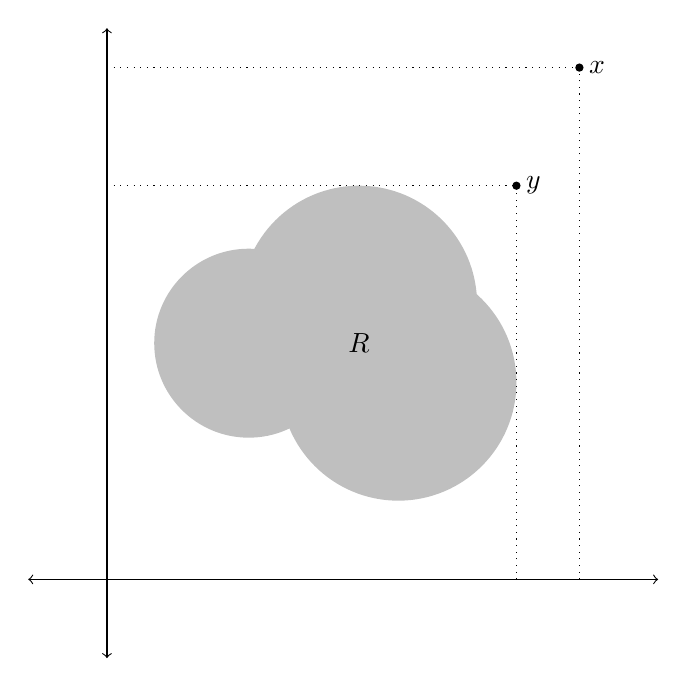
\begin{tikzpicture}[scale=1]
	
	% blob
	\fill[lightgray] (3.2,3.5) circle[radius=1.5cm];
	\fill[lightgray] (3.7,2.5) circle[radius=1.5cm];
	\fill[lightgray] (1.8,3) circle[radius=1.2cm];
	\draw (3.2,3) node {$R$} ;

	% \widebar{a}
	\draw (6,6.5) node[anchor=west] {$x$} ;
	\fill (6,6.5) circle[radius=1.5pt];
	\draw[dotted] (6,0) -- (6,6.5);
	\draw[dotted] (0,6.5) -- (6,6.5);

	% a^*
	\draw (5.2,5) node[anchor=west] {$y$} ;
	\fill (5.2,5) circle[radius=1.5pt];
	\draw[dotted] (5.2,0) -- (5.2,5);
	\draw[dotted] (0,5) -- (5.2,5);

	% axes
	\draw[<->] (-1,0) -- (7,0);
	\draw[<->] (0,-1) -- (0,7);

\end{tikzpicture}
	\caption{The poset $\left(\R^2,\geq\right)$ and a subset $R \subseteq \R^2$. $x$ is an upper bound of $R$ in $\left(\R^2,\geq\right)$, and $y$ is the least upper bound (supremum) of $R$ in $\left(\R^2,\geq\right)$.}
	\label{fig:example_supremum}	
\end{figure}


\begin{definition}
	%
	A poset $(L,\gtrsim)$ is a lattice iff
	%
	\begin{equation*}
		\sup_{(L,\gtrsim)}\{x,y\}
		\quad\text{and}\quad
		\inf_{(L,\gtrsim)}\{x,y\}
	\end{equation*}
	%
	exist for every pair $x,y \in L$.
	%
\end{definition}

We will sometimes be sloppy and refer to a set $L$ as a poset or lattice, suppressing the order (as we often do with topologies, metrics, etc.)


\begin{definition}
	%
	A lattice $(L,\gtrsim)$ is complete iff
	%
	\begin{equation*}
		\sup_{(L,\gtrsim)} R
		\quad\text{and}\quad
		\inf_{(L,\gtrsim)} R
	\end{equation*}
	%
	exist for every $R \subseteq L$.%
		\footnote{Some authors use `complete' to mean something weaker. We follow the convention from \textcite{Topkis1998}.}
	%
\end{definition}


\begin{example}
	%
	The posets $\left([0,1]^n,\geq\right)$ and $(\{1,2,\dots,k\}^n,\geq)$ are complete lattices. $\left(\R^n,\geq\right)$, $\left((0,1)^n,\geq\right)$, $((\Q \cap [0,1])^n,\geq)$ and $\left(\N^n,\geq\right)$ are also a lattices, but it are not complete.
	%
\end{example}

\begin{example}
	%
	For any set $\Omega$, $\left( 2^\Omega, \supseteq \right)$ is a complete lattice.
	%
\end{example}

We can generalise these examples as follows. Let $\{ (L_i,\gtrsim_i) \}_{i \in I}$ be a collection of lattices, set $L \coloneqq \prod_{i \in I} L_i$ and define $\gtrsim$ on $L$ by $x \gtrsim y$ iff $x_i \gtrsim_i y_i$ for each $i \in I$. $(L,\gtrsim)$ thus defined is called a product lattice. As the name suggests, a product lattice is a lattice. Clearly $\left(\R^n,\geq\right)$ is a product lattice. So is $\bigl( 2^\Omega, \supseteq \bigr)$: it is the product of lattices $(\{0,1\},\geq)$.

\begin{example}
	%
	Let $\Delta([a,b])$ denote the set of Borel probability measures on $[a,b]$, and let $\gtrsim_F$ be the first-order stochastic dominance order on $\Delta([a,b])$. $\left( \Delta([a,b]), \gtrsim_F \right)$ is a complete lattice.
	%
\end{example}


We now consider the lattice structure of subsets of lattices. For a poset $(L,\gtrsim)$ and a subset $R \subseteq L$, let $\gtrsim|_R$ be the restriction of $\gtrsim$ to $R$. Clearly $(R,\gtrsim|_R)$ is also a poset. To save ourselves some pain, we will henceforth be sloppy and write simply $(R,\gtrsim)$, taking it as understood that $\gtrsim$ is restricted to the appropriate domain.
%
\begin{definition}
	%
	Let $(L,\gtrsim)$ be a lattice and $L' \subseteq L$. $(L',\gtrsim)$ is a sublattice of $(L,\gtrsim)$ iff for any $x,y \in L'$, $\sup_{(L,\gtrsim)}\{x,y\}$ and $\inf_{(L,\gtrsim)}\{x,y\}$ lie in $L'$.
	%
\end{definition}

\noindent \Cref{fig:example_sublattice} gives some examples of sublattices and non-sublattices.
%
\begin{figure}
	\begin{subfigure}{0.5\textwidth}
		\centering
		% Copyright (c) 2020 Carl Martin Ludvig Sinander.

% This program is free software: you can redistribute it and/or modify
% it under the terms of the GNU General Public License as published by
% the Free Software Foundation, either version 3 of the License, or
% (at your option) any later version.

% This program is distributed in the hope that it will be useful,
% but WITHOUT ANY WARRANTY; without even the implied warranty of
% MERCHANTABILITY or FITNESS FOR A PARTICULAR PURPOSE. See the
% GNU General Public License for more details.

% You should have received a copy of the GNU General Public License
% along with this program. If not, see <https://www.gnu.org/licenses/>.

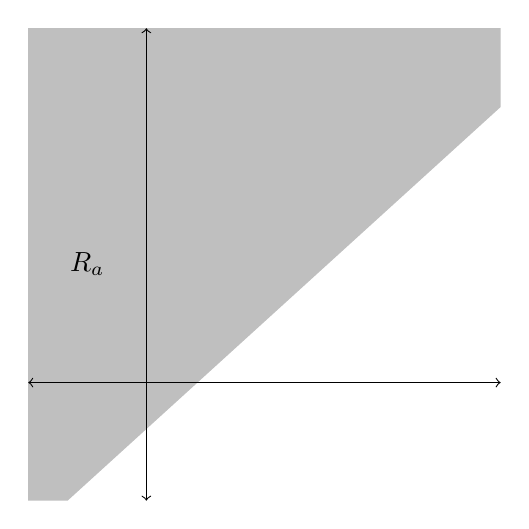
\begin{tikzpicture}[scale=1]
	
	% S'
	\fill[lightgray] (-1,-1.5) -- (4.5,3.5) -- (4.5,4.5) -- (-1.5,4.5) -- (-1.5,-1.5) -- (-1,-1.5);
	\draw (-0.75,1.5) node {$R_a$};

	% % points
	% \fill (0.75,2) circle[radius=1.5pt];
	% \fill (2.75,2) circle[radius=1.5pt];
	% \fill (2.75,3.5) circle[radius=1.5pt];
	% \fill (0.75,3.5) circle[radius=1.5pt];

	% % point labels
	% \draw (0.75,2) node[anchor=north] {$x' \meet x''$};
	% \draw (2.75,2) node[anchor=north] {$x''$};
	% \draw (2.75,3.5) node[anchor=south] {$x' \join x''$};
	% \draw (0.75,3.5) node[anchor=south] {$x'$};

	% ax'es
	\draw[<->] (-1.5,0) -- (4.5,0);
	\draw[<->] (0,-1.5) -- (0,4.5);

\end{tikzpicture}
		\caption{}
	\end{subfigure}
	\begin{subfigure}{0.5\textwidth}
		\centering
		\input{tikz/example_sublattice_b}
		\caption{}
	\end{subfigure}
	\\
	\begin{subfigure}{0.5\textwidth}
		\centering
		\input{tikz/example_sublattice_c}
		\caption{}
	\end{subfigure}
	\begin{subfigure}{0.5\textwidth}
		\centering
		% Copyright (c) 2020 Carl Martin Ludvig Sinander.

% This program is free software: you can redistribute it and/or modify
% it under the terms of the GNU General Public License as published by
% the Free Software Foundation, either version 3 of the License, or
% (at your option) any later version.

% This program is distributed in the hope that it will be useful,
% but WITHOUT ANY WARRANTY; without even the implied warranty of
% MERCHANTABILITY or FITNESS FOR A PARTICULAR PURPOSE. See the
% GNU General Public License for more details.

% You should have received a copy of the GNU General Public License
% along with this program. If not, see <https://www.gnu.org/licenses/>.

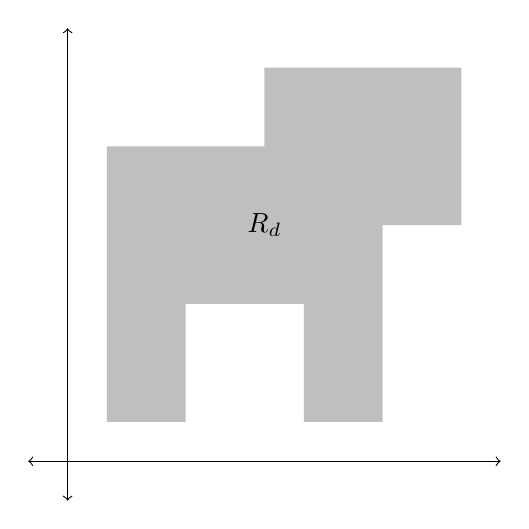
\begin{tikzpicture}[scale=1]
	
	% S'
	\fill[lightgray] (0.5,0.5) -- (1.5,0.5) -- (1.5,2) -- (3,2) -- (3,0.5) -- (4,0.5) -- (4,3) -- (5,3) -- (5,5) -- (2.5,5) -- (2.5,4) -- (0.5,4) -- (0.5,0.5);
	\draw (2.5,3) node {$R_d$};

	% axes
	\draw[<->] (-0.5,0) -- (5.5,0);
	\draw[<->] (0,-0.5) -- (0,5.5);

\end{tikzpicture}
		\caption{}
	\end{subfigure}
	\caption{The lattice $\left(\R^2,\geq\right)$ and four subsets. $(R_a,\geq)$ and $(R_b,\geq)$ are sublattices of $\left(\R^2,\geq\right)$, whereas $(R_c,\geq)$ and $(R_d,\geq)$ are not. (In fact, the latter two are not even lattices in their own right.)}
	\label{fig:example_sublattice}
\end{figure}


Obviously any sublattice is itself a lattice. But the converse is not true!
%
\begin{example}
	%
	Let $L \coloneqq \{ (1/2,1/2),(2,1),(1,2),(3,3) \}$, as drawn in \Cref{fig:example_sublattice3}.
	%
	\begin{figure}
		\centering
		% Copyright (c) 2020 Carl Martin Ludvig Sinander.

% This program is free software: you can redistribute it and/or modify
% it under the terms of the GNU General Public License as published by
% the Free Software Foundation, either version 3 of the License, or
% (at your option) any later version.

% This program is distributed in the hope that it will be useful,
% but WITHOUT ANY WARRANTY; without even the implied warranty of
% MERCHANTABILITY or FITNESS FOR A PARTICULAR PURPOSE. See the
% GNU General Public License for more details.

% You should have received a copy of the GNU General Public License
% along with this program. If not, see <https://www.gnu.org/licenses/>.

\begin{tikzpicture}[scale=2]
	
	% points
	\fill[gray] (0.5,0.5) circle[radius=0.75pt];
	\fill[gray] (2,1) circle[radius=0.75pt];
	\fill[gray] (1,2) circle[radius=0.75pt];
	\fill[gray] (3,3) circle[radius=0.75pt];

	% labels
	\draw (0.5,0) node[anchor=north] {$\tfrac{1}{2}$};
	\draw (0,0.5) node[anchor=east] {$\tfrac{1}{2}$};
	\draw (1,0) node[anchor=north] {$1$};
	\draw (0,1) node[anchor=east] {$1$};
	\draw (2,0) node[anchor=north] {$2$};
	\draw (0,2) node[anchor=east] {$2$};
	\draw (3,0) node[anchor=north] {$3$};
	\draw (0,3) node[anchor=east] {$3$};

	% axes
	\draw[<->] (-0.5,0) -- (3.5,0);
	\draw[<->] (0,-0.5) -- (0,3.5);

\end{tikzpicture}
		\caption{The set $L = \{ (\tfrac{1}{2},\tfrac{1}{2}), (2,1), (1,2), (3,3) \} \subseteq \R^2$. $(L,\geq)$ is a lattice, but it is not a sublattice of $\left(\R^2,\geq\right)$.}
		\label{fig:example_sublattice3}
	\end{figure}
	%
	$(L,\geq)$ is not a sublattice of $\left(\R^2,\geq\right)$ since for example
	%
	\begin{equation*}
		\sup_{(\R^2,\geq)} \{ (2,1), (1,2) \} = (2,2) \notin L .
	\end{equation*}
	%
	It is a lattice, though; for example, $\sup_{(L,\geq)} \{ (2,1), (1,2) \} = (3,3)$.
	%
\end{example}


For $1 \leq i < j \leq n$, let $\pi_{ij} : \R^n \to \R^2$ be the projection map
%
\begin{equation*}
	\pi_{ij}(x_1,\dots,x_i,\dots,x_j,\dots,x_n) = (x_i,x_j) .
\end{equation*}
%
The following theorem says that for `Euclidean' lattices $\left(\R^n,\geq\right)$, the sublattice property holds iff it holds for every pair of dimensions.

\begin{theorem}
	%
	\label{theorem:sublattice_pairwise}
	%
	Let $(L,\geq)$ be a sublattice of $\left(\R^n,\geq\right)$, and take $x \in \R^n$. Then $x \in L$ iff $\pi_{ij}(x) \in \pi_{ij}(L)$ for all $1 \leq i < j \leq n$.
	%
\end{theorem}


\begin{proof}
	%
	Let $(L,\geq)$ be a sublattice of $\left(\R^n,\geq\right)$, and take $x \in \R^n$. It's obvious that $x \in L$ implies $\pi_{ij}(x) \in \pi_{ij}(L)$ for any $1 \leq i < j \leq n$.

	Let $\{ v_{ij} \}_{1 \leq i < j \leq n}$ be vectors in $\R^n$ such that $\pi_{ij}(v_{ij})=\pi_{ij}(x) \in \pi_{ij}(L)$. Fix $i \in \{1,\dots,n\}$, and consider 
	%
	\begin{equation*}
		V_i \coloneqq \sup_{(\R^n,\geq)} 
		\{ v_{i1},\dots,v_{i,j-1},v_{i,j+1},\dots,v_{in} \} .
	\end{equation*}
	%
	The $i$th coordinate of $V_i$ obviously equals $x_i$. The $j$th coordinate for $j \neq i$ is weakly greater than the $j$th coordinate of $x$. It follows that
	%
	\begin{equation*}
		\inf_{(\R^n,\geq)} \left\{ V_1,\dots,V_n \right\} = x .
	\end{equation*}
	%
	Since $(L,\geq)$ is a sublattice of $\left(\R^n,\geq\right)$, $\inf_{(\R^n,\geq)} \left\{ V_1,\dots,V_n \right\} \in L$; hence $x \in L$.
	%
\end{proof}


\begin{definition}
	%
	Let $(L,\gtrsim)$ be a complete lattice and $(L',\gtrsim)$ a sublattice of it. $(L',\gtrsim)$ is subcomplete iff for every $R \subseteq L'$, $\sup_{(L',\gtrsim)} R$ and $\inf_{(L',\gtrsim)} R$ lie in $L'$.
	%
\end{definition}

A subcomplete sublattice is a sublattice. A subcomplete sublattice is also a complete lattice in its own right. But the converse is false!
%
\begin{example}
	%
	Let $L \coloneqq \{0\} \union (1/2,1]$. $(L,\geq)$ is a sublattice of $(\R,\geq)$, and is a complete lattice in its own right. (Convince yourself.) But it is not a subcomplete sublattice of $(\R,\geq)$ since
	%
	\begin{equation*}
		\inf_{(\R,\geq)} (1/2,1] = 1/2 \notin L .
	\end{equation*}
	%
\end{example}


\begin{theorem}
	%
	A sublattice $(L,\geq)$ of $\left(\R^n,\geq\right)$ is subcomplete iff $L$ is compact.
	%
\end{theorem}

The proof is straightforward, and perhaps a good exercise.



%%%%%%%%%%%%%%%%%%%%%%%%%%%%%%%%%%%%%%%%%
\subsection{Tarski's fixed-point theorem}
\label{sec:supermodular:tarski}
%%%%%%%%%%%%%%%%%%%%%%%%%%%%%%%%%%%%%%%%%

\begin{definition}
	%
	Let $(L,\gtrsim)$ be a poset. A map $f : L \to L$ is increasing (or monotone, or $\gtrsim$-order-preserving) iff $x \gtrsim y$ implies $f(x) \gtrsim f(y)$.
	%
\end{definition}

We are interested in the set $\{ x \in L : f(x) = x \}$ of fixed points of an increasing function $f$. We have the following beautiful theorem.

\begin{theorem}[\textcite{Tarski1955}]
	%
	\label{theorem:Tarski}
	%
	If $(L,\gtrsim)$ is a nonempty complete lattice and $f : L \to L$ is order-preserving, then the set of fixed points of $f$ is a nonempty complete lattice with greatest and least elements
	%
	\begin{equation*}
		\sup_{(L,\gtrsim)} \left\{ x \in L : x \lesssim f(x) \right\}
		\quad\text{and}\quad
		\inf_{(L,\gtrsim)} \left\{ x \in L : x \gtrsim f(x) \right\} .
	\end{equation*}
	%
\end{theorem}

\noindent \Cref{fig:brouwer_vs_tarski} illustrates the theorem and compares it with Brouwer's (\citeyear{Brouwer1912}) fixed-point theorem.
%
\begin{figure}
	\begin{subfigure}{0.5\textwidth}
		\centering
		% Copyright (c) 2020 Carl Martin Ludvig Sinander.

% This program is free software: you can redistribute it and/or modify
% it under the terms of the GNU General Public License as published by
% the Free Software Foundation, either version 3 of the License, or
% (at your option) any later version.

% This program is distributed in the hope that it will be useful,
% but WITHOUT ANY WARRANTY; without even the implied warranty of
% MERCHANTABILITY or FITNESS FOR A PARTICULAR PURPOSE. See the
% GNU General Public License for more details.

% You should have received a copy of the GNU General Public License
% along with this program. If not, see <https://www.gnu.org/licenses/>.

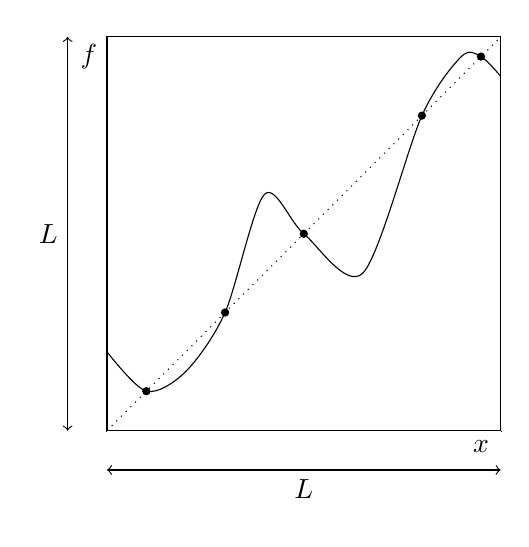
\begin{tikzpicture}[scale=1]
	
	% X
	\draw[<->] (0,-0.5)--(5,-0.5);
	\draw[<->] (-0.5,0)--(-0.5,5);
	\draw (-0.5,2.5) node[anchor=east] {$L$};
	\draw (2.5,-0.5) node[anchor=north] {$L$};

	% invisible corners
	\draw (-1,-1) node[anchor=west] {};
	\draw (5,-1) node[anchor=east] {};
	\draw (-1,5) node[anchor=west] {};

	% diagonal line
	\draw[-,dotted] (0,0)--(5,5);

	% function
	\draw plot [smooth] coordinates {(0,1) (0.5,0.5) (1,0.75) (1.5,1.5) (2,3) (2.5,2.5) (3.25,2) (4,4) (4.5,4.75) (4.75,4.75) (5,4.5)};

	% fixed points
	\fill (0.5,0.5) circle[radius=1.5pt];
	\fill (1.5,1.5) circle[radius=1.5pt];
	\fill (2.5,2.5) circle[radius=1.5pt];
	\fill (4,4) circle[radius=1.5pt];
	\fill (4.75,4.75) circle[radius=1.5pt];

	% axes
	\draw[-] (0,0)--(5,0);
	\draw[-] (0,0)--(0,5);
	\draw[-] (5,5)--(5,0);
	\draw[-] (5,5)--(0,5);

	% axis labels
	\draw (0,4.75) node[anchor=east] {$f$};
	\draw (4.75,0) node[anchor=north] {$x$};

	% fix up corners
	\fill (-0.007,-0.007) rectangle (0.001,0.001);
	\fill (5.007,-0.007) rectangle (4.999,0.001);
	\fill (-0.007,5.007) rectangle (0.001,4.999);
	\fill (5.007,5.007) rectangle (4.993,4.993);

\end{tikzpicture}
		\caption{}
	\end{subfigure}
	\begin{subfigure}{0.5\textwidth}
		\centering
		% Copyright (c) 2020 Carl Martin Ludvig Sinander.

% This program is free software: you can redistribute it and/or modify
% it under the terms of the GNU General Public License as published by
% the Free Software Foundation, either version 3 of the License, or
% (at your option) any later version.

% This program is distributed in the hope that it will be useful,
% but WITHOUT ANY WARRANTY; without even the implied warranty of
% MERCHANTABILITY or FITNESS FOR A PARTICULAR PURPOSE. See the
% GNU General Public License for more details.

% You should have received a copy of the GNU General Public License
% along with this program. If not, see <https://www.gnu.org/licenses/>.

\begin{tikzpicture}[scale=1]
	
	% X
	\draw[<->] (0,-0.5)--(5,-0.5);
	\draw[<->] (-0.5,0)--(-0.5,5);
	\draw (-0.5,2.5) node[anchor=east] {$L$};
	\draw (2.5,-0.5) node[anchor=north] {$L$};

	% invisible corners
	\draw (-1,-1) node[anchor=west] {};
	\draw (5,-1) node[anchor=east] {};
	\draw (-1,5) node[anchor=west] {};

	% diagonal line
	\draw[-,dotted] (0,0)--(5,5);

	% function
	\draw[-] (0,0.5)--(1,1)--(2,1.5);
	\draw[-] (2,2.5)--(3,3)--(4,3.5);
	\draw[-] (4,4.25)--(4.5,4.5)--(5,4.75);

	% fixed points
	\fill (1,1) circle[radius=1.5pt];
	\fill (3,3) circle[radius=1.5pt];
	\fill (4.5,4.5) circle[radius=1.5pt];

	% axes
	\draw[-] (0,0)--(5,0);
	\draw[-] (0,0)--(0,5);
	\draw[-] (5,5)--(5,0);
	\draw[-] (5,5)--(0,5);

	% axis labels
	\draw (0,4.75) node[anchor=east] {$f$};
	\draw (4.75,0) node[anchor=north] {$x$};

	% fix up corners
	\fill (-0.007,-0.007) rectangle (0.001,0.001);
	\fill (5.007,-0.007) rectangle (4.999,0.001);
	\fill (-0.007,5.007) rectangle (0.001,4.999);
	\fill (5.007,5.007) rectangle (4.993,4.993);

\end{tikzpicture}
		\caption{}
	\end{subfigure}
	\caption{Two functions $f : L \to L$, where $L$ is a compact and convex subset of $\R$ and (hence) $(L,\geq)$ is a complete lattice. Panel (a) illustrates Brouwer's fixed point theorem, which requires continuity of $f$. Panel (b) depicts Tarski's fixed-point theorem, which requires that $f$ be increasing.}
	\label{fig:brouwer_vs_tarski}
\end{figure}

For $L$ finite, it's obvious why this is true. Since $L$ is a nonempty complete lattice, it has a smallest element $x_0 \in L$. For each $n \in \N$, define $x_n = f(x_{n-1})$. By monotonicity, $x_n = f(x_{n-1}) \gtrsim x_{n-1}$ for each $n \in \N$. By finiteness, strict improvements must eventually stop, leaving us with a fixed point.

The fact that the result holds for arbitrary $L$ is what makes the theorem deep. We'll just prove the existence of a fixed point. (But the other steps are entirely straightforward.)
%
\begin{proof}[Proof of existence]
	%
	Define
	%
	\begin{equation*}
		R \coloneqq \left\{ x \in L : x \gtrsim f(x) \right\} .
	\end{equation*}
	%
	$R$ is nonempty since $\sup_{(L,\gtrsim)} L \in R$. Define $x_\star \coloneqq \inf_{(L,\gtrsim)} R$; $x_\star$ is well-defined since $R$ is nonempty and $(L,\gtrsim)$ is complete.

	Take any $x \in R$; then $x_\star \lesssim x$, so $f(x_\star) \lesssim f(x)$ by monotonicity. Since $f(x) \lesssim x$ by definition of $R$, it follows that $f(x_\star) \lesssim x$ for any $x \in R$, so that $f(x_\star)$ is a lower bound of $R$. Since $x_\star$ is the greatest lower bound of $R$ (by definition), $x_\star \gtrsim f(x_\star)$.

	Hence $x_\star \in R$, so that $x_\star \gtrsim f(x_\star)$. By monotonicity, it follows that $f(x_\star) \gtrsim f(f(x_\star))$, and hence $f(x_\star) \in R$ by definition of $R$. Since $x_\star$ is a lower bound of $R$, it follows that $x_\star \lesssim f(x_\star)$.

	Since $\gtrsim$ is antisymmetric, we conclude that $x_\star = f(x_\star)$.
	%
\end{proof}


Tarski's fixed-point theorem can be used for all kinds of things. Some familiar examples are as follows.

\begin{example}[best-reply sets]
	%
	Consider a game $(I,\{A_i,u_i\}_{i \in I})$ in normal form. Let $B_i(A_{-i}')$ denote the set of best responses $\in A_i$ to conjectures supported on $A_{-i}' \subseteq A_{-i}$. Write $A \coloneqq \prod_{i \in I} A_i$ and $B(A) \coloneqq ( B_i(A_{-i}) )_{i \in I}$. A product set $A' \coloneqq \prod_{i \in I} A_i' \subseteq A$ has the best-reply property iff for any profile $(a_i)_{i \in I} \in A'$ and any player $i \in I$, $a_i$ is a best reply to some conjecture supported on $A_{-i}'$. More succinctly, $A'$ has the best-reply property iff $A' \subseteq B(A')$.

	Let $\mathcal{P}(A)$ denote the product subsets of $A$. $( \mathcal{P}(A), \supseteq )$ is clearly a complete lattice, and $B : \mathcal{P}(A) \to \mathcal{P}(A)$ is clearly $\supseteq$-order-preserving. Hence by Tarski's fixed-point theorem, $B$ has a largest fixed point. It follows that there is a largest best-reply set $R$ ($R$ is a best-reply set and contains every other best-reply set).

	For $k \in \N$, let $A^k$ be the (product) set of strategy profiles surviving $k$ rounds of deletion of never-best-replies, so that $A^\infty \coloneqq \Intersect_{k \in \N} A^k$ is the rationalisable set. Clearly $A^k \supseteq R$ for each $k \in \N$, hence $A^\infty \supseteq R$. Each $A^k$ has the best-reply property by definition, and if action spaces are compact and payoffs continuous,%
		\footnote{Finite action spaces (with the discrete topology) are a special case.}
	then the best-reply property is preserved under countable interesection, so $A^\infty \subseteq B(A^\infty)$. It follows that $A^\infty=R$, i.e. the rationalisable set concides with the maximal best-reply set.%
		\footnote{Note that the existence, nonemptiness and properties of the largest best-reply set requires no assumptions at all on the game. By contrast, the nonemptiness and properties of the rationalisable set rely on topological structure.}
	%
\end{example}

\begin{example}[repeated games]
	%
	Consider a repeated game with imperfect monitoring, and let the set of players be $I$. As in \textcite{AbreuPearceStacchetti1990}, let $B(W) \subseteq \R^{\abs*{I}}$ denote the set of payoff profiles generated by the payoff profiles $W \subseteq \R^{\abs*{I}}$.
	A set $W \subseteq \R^{\abs*{I}}$ is called self-generating iff $W \subseteq B(W)$.

	Clearly $\bigl( 2^{\R^n}, \supseteq \bigr)$ is a complete lattice and $B$ is $\supseteq$-order-preserving. Hence by Tarski's theorem, $B$ has a largest fixed point: there is a self-generating set $W^\star$ that contains all other self-generating sets. $W^\star$ is the set of all PPE payoff vectors.
	%
\end{example}

\begin{example}[Markov chains]
	%
	Consider a Markov chain on $[a,b]$ with transition kernel $f : [a,b] \to \Delta([a,b])$.%
		\footnote{$\Delta([a,b])$ are the Borel measures on $[a,b]$, remember.}
	The induced Markov operator $T : \Delta([a,b]) \to \Delta([a,b])$ is given by
	%
	\begin{equation*}
		(T\mu)(E) \coloneqq \int_{[a,b]} f(E|x) \mu(\dd x)
		\quad\text{for every $E\subseteq [a,b]$ Borel} .
	\end{equation*}
	%
	$\mu \in \Delta([a,b])$ is an invariant distribution of the Markov chain iff it is a fixed point of $T$.

	Let's assume that $x \geq y$ implies $f(x) \gtrsim_F f(y)$, where $\gtrsim_F$ is the first-order stochastic dominance order. This obviously implies that $T$ is $\gtrsim_F$-order-preserving. We already know that $( \Delta([a,b]), \gtrsim_F )$ is a complete lattice. It follows by Tarski's theorem that the Markov chain has an invariant distribution, and further that its invariant distributions form a complete lattice with respect to first-order stochastic dominance.%
		\footnote{The other obvious way to guarantee the existence of an invariant distribution is to impose continuity and compactness assumptions, then to appeal to Brouwer's fixed-point theorem. The natural route would be to endow $\Delta([a,b])$ with the weak$^\star$ topology (that gives us compactness for free) and to assume that $f$ is continuous.}
	%
\end{example}


\begin{example}[matching]
	%
	Let $W$ and $M$ be sets of heterosexual women and men, respectively. For simplicity, assume that $\abs*{W}=\abs*{M}=n$. Each woman $w \in W$ has a strict preference relation $\succ_w$ on $M$,%
		\footnote{`Strict preference order' here just means `total order'.}
	and similarly men $m \in M$ have preferences $\succ_m$ over $W$.

	A matching is a map $\mu : W \union M \to W \union M$ such that $\mu(W) \subseteq M$ and $\mu(M) \subseteq W$ (heteronormativity) and $\mu \circ \mu$ is the identity (consistency). A matching $\mu$ is stable iff there is no pair $(w,m) \in W \times M$ s.t. $m \succ_w \mu(w)$ and $w \succ_m \mu(m)$.

	A prematching is a pair $(f,g)$ of maps $f : W \to M \union \{\varnothing\}$ and $g : M \to W \union \{\varnothing\}$. (Unlike a matching, a prematching allows people to remain single, and doesn't impose consistency.) Let $L$ be the set of all prematchings, and write $(f,g) \gtrsim (f',g')$ iff all women weakly prefer $f$ to $f'$ and all men weakly prefer $g'$ to $g$. %(In symbols: $f(w) \succeq_w f'(w)$ for each $w \in W$ and $g(m) \succeq_m g'(m)$ for each $m \in M$.)
	Surprisingly (at least to me), $(L,\gtrsim)$ is a complete lattice. (The proof is not hard.)

	For a prematching $(f,g)$, let $Tf$ be the map $W \to M \union \{\varnothing\}$ we get by letting each woman $w$ grab her favourite man from among those who are either single or are willing to leave their present spouse under $g$ for $w$, and similarly for $Tg$. Formally, $T : L \to L$ is given by
	%
	\begin{align*}
		Tf(w) \coloneqq{}& \max_{\succ_w} \left\{
		m \in M :
		\text{$g(m) = \varnothing$ or $w \succeq_m g(m)$}
		\right\}
		\\
		Tg(m) \coloneqq{}& \max_{\succ_m} \left\{
		w \in W :
		\text{$f(w) = \varnothing$ or $m \succeq_w f(w)$}
		\right\} .
	\end{align*}
	%
	An application of $T$ to a prematching is essentially equivalent to one round of the Gale--Shapley (\citeyear{GaleShapley1962}) algorithm. A moment's reflection reveals that $T$ is $\gtrsim$-order-preserving.

	It follows by Tarski's fixed-point theorem that the set $R$ of fixed points of $T$ is a nonempty complete lattice w.r.t. $\gtrsim$. Fixed points of $T$ clearly correspond to stable matchings, so we've shown not only that stable matchings exist, but that there is a stable matching preferred by all women (viz. $\sup_{(L,\gtrsim)} R$) and a stable matching preferred by all men ($\inf_{(L,\gtrsim)} R$). The latter result is not obvious, nor even intuitive! (I would say.)

	Since $L$ is finite, starting at the smallest or largest prematching and iterating on $T$ yields a stable matching in finite time. Starting the algorithm at the largest prematching will generate the women-favoured matching, and starting at the smallest prematching yields the men-preferred matching.%
		\footnote{The lattice structure of stable matchings was first pointed out in print by \textcite{Knuth1976} (that's the guy who invented \TeX!), but he attributes the discovery to John Conway.}
	%
\end{example}


To study best-response correspondences and hence Nash equilibria, we will require an extension of Tarski's theorem to correspondences. To do that, we need an appropriate notion of monotonicity for correspondences, which in turn requires an order on sublattices.
%
\begin{definition}
	%
	Let $\mathcal{P}(L,\gtrsim)$ be the set of sublattices of a lattice $(L,\gtrsim)$. The strong set order induced by $(L,\gtrsim)$ is the order $\sqsupseteq$ on $\mathcal{P}(L,\gtrsim)$ such that $(L',\gtrsim) \sqsupseteq (L'',\gtrsim)$ iff for any $x' \in L'$ and $x'' \in L''$, $\sup_{(L,\gtrsim)}\{x',x''\} \in L'$ and $\inf_{(L,\gtrsim)}\{x',x''\} \in L''$.
	%
\end{definition}

\noindent \Cref{fig:example_strong_set_order} illustrates the strong set order.
%
\begin{figure}
	\begin{subfigure}{0.5\textwidth}
		\centering
		% Copyright (c) 2020 Carl Martin Ludvig Sinander.

% This program is free software: you can redistribute it and/or modify
% it under the terms of the GNU General Public License as published by
% the Free Software Foundation, either version 3 of the License, or
% (at your option) any later version.

% This program is distributed in the hope that it will be useful,
% but WITHOUT ANY WARRANTY; without even the implied warranty of
% MERCHANTABILITY or FITNESS FOR A PARTICULAR PURPOSE. See the
% GNU General Public License for more details.

% You should have received a copy of the GNU General Public License
% along with this program. If not, see <https://www.gnu.org/licenses/>.

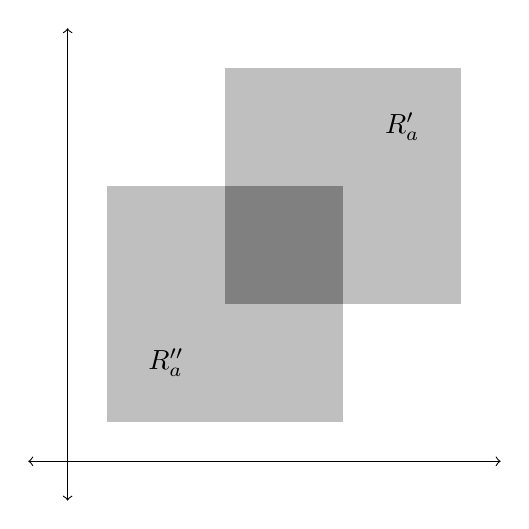
\begin{tikzpicture}[scale=1]
	
	% S'
	\fill[lightgray] (0.5,0.5)--(3.5,0.5)--(3.5,3.5)--(0.5,3.5);
	\draw (1.25,1.25) node {$R_a''$};

	% S''
	\fill[lightgray] (2,2)--(5,2)--(5,5)--(2,5);
	\draw (4.25,4.25) node {$R_a'$};

	% overlap
	\fill[gray] (2,2)--(3.5,2)--(3.5,3.5)--(2,3.5);

	% axes
	\draw[<->] (-0.5,0) -- (5.5,0);
	\draw[<->] (0,-0.5) -- (0,5.5);

\end{tikzpicture}
		\caption{}
	\end{subfigure}
	\begin{subfigure}{0.5\textwidth}
		\centering
		% Copyright (c) 2020 Carl Martin Ludvig Sinander.

% This program is free software: you can redistribute it and/or modify
% it under the terms of the GNU General Public License as published by
% the Free Software Foundation, either version 3 of the License, or
% (at your option) any later version.

% This program is distributed in the hope that it will be useful,
% but WITHOUT ANY WARRANTY; without even the implied warranty of
% MERCHANTABILITY or FITNESS FOR A PARTICULAR PURPOSE. See the
% GNU General Public License for more details.

% You should have received a copy of the GNU General Public License
% along with this program. If not, see <https://www.gnu.org/licenses/>.

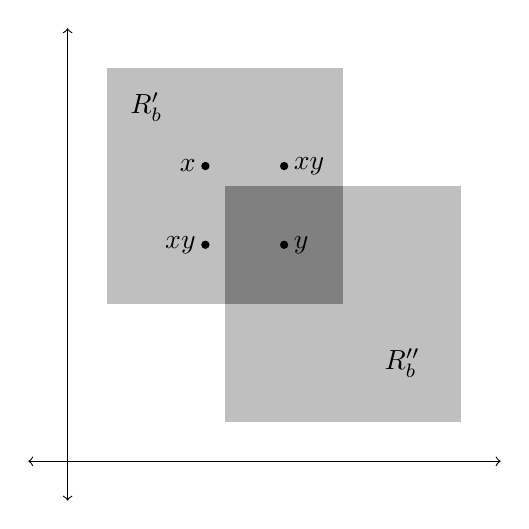
\begin{tikzpicture}[scale=1]
	
	% S'
	\fill[lightgray] (2,0.5)--(5,0.5)--(5,3.5)--(2,3.5);
	\draw (4.25,1.25) node {$R_b''$};

	% S''
	\fill[lightgray] (0.5,2)--(3.5,2)--(3.5,5)--(0.5,5);
	\draw (1,4.5) node {$R_b'$};

	% overlap
	\fill[gray] (2,2)--(3.5,2)--(3.5,3.5)--(2,3.5);

	% points
	\fill (1.75,2.75) circle[radius=1.5pt];
	\fill (2.75,2.75) circle[radius=1.5pt];
	\fill (2.75,3.75) circle[radius=1.5pt];
	\fill (1.75,3.75) circle[radius=1.5pt];

	% point labels
	\draw (1.75,2.75) node[anchor=east] {$x \meet y$};
	\draw (2.75,2.75) node[anchor=west] {$y$};
	\draw (2.75,3.75) node[anchor=west] {$x \join y$};
	\draw (1.75,3.75) node[anchor=east] {$x$};

	% axes
	\draw[<->] (-0.5,0) -- (5.5,0);
	\draw[<->] (0,-0.5) -- (0,5.5);

\end{tikzpicture}
		\caption{}
	\end{subfigure}
	\caption{The lattice $\left(\R^2,\geq\right)$ and some sublattices. In panel (a), $R_a' \sqsupseteq R_a''$. In panel (b), $R_b'$ and $R_b''$ are not ranked by the strong set order.}
	\label{fig:example_strong_set_order}
\end{figure}

\begin{definition}
	%
	Let $(L,\gtrsim)$ be a lattice, and let $\sqsupseteq$ be the strong order it induces on $\mathcal{P}(L,\gtrsim)$. A correspondence $f : L \Rightarrow L$ is increasing (in the induced order) iff it is sublattice-valued and $x \gtrsim y$ implies $f(x) \sqsupseteq f(y)$.%
		\footnote{If we view the correspondence $f$ as a set-valued function, then this definition says that $f$ must be sublattice-valued and $\sqsupseteq$-order-preserving.}
	%
\end{definition}


\begin{theorem}[\textcite{Zhou1994}]
	%
	\label{theorem:Zhou}
	%
	If $(L,\gtrsim)$ is a nonempty complete lattice and $f : L \Rightarrow L$ is increasing in the induced order, then the set of fixed points of $f$ is a nonempty complete lattice.
	%
\end{theorem}



%%%%%%%%%%%%%%%%%%%%%%%%%%%%%%%%%%%%%%%%%%
\subsection{Topkis's monotonicity theorem}
\label{sec:supermodular:supermodular_fns}
%%%%%%%%%%%%%%%%%%%%%%%%%%%%%%%%%%%%%%%%%%

\begin{definition}
	%
	Let $(L,\gtrsim)$ and $(L',\gtrsim')$ be posets. $f : L \times L' \to \R$ has increasing differences iff whenever $x \gtrsim x'$, $\delta(\cdot) \coloneqq f(x,\cdot)-f(x',\cdot)$ is increasing in $\gtrsim'$.
	%
\end{definition}

\begin{definition}
	%
	Let $(L,\gtrsim)$ be a lattice. $f : L \to \R$ is supermodular iff for any $x,x' \in L$,
	%
	\begin{equation*}
		f\left( \sup_{(L,\gtrsim)}\{x,x'\} \right) 
		+ f\left( \inf_{(L,\gtrsim)}\{x,x'\} \right) 
		\geq f(x) + f(x') .
	\end{equation*}
	%
\end{definition}

\noindent For those who like pictures, \Cref{fig:example_supermodularity} illustrates what a supermodular function looks like.
%
\begin{figure}
	\centering
	% Copyright (c) 2020 Carl Martin Ludvig Sinander.

% This program is free software: you can redistribute it and/or modify
% it under the terms of the GNU General Public License as published by
% the Free Software Foundation, either version 3 of the License, or
% (at your option) any later version.

% This program is distributed in the hope that it will be useful,
% but WITHOUT ANY WARRANTY; without even the implied warranty of
% MERCHANTABILITY or FITNESS FOR A PARTICULAR PURPOSE. See the
% GNU General Public License for more details.

% You should have received a copy of the GNU General Public License
% along with this program. If not, see <https://www.gnu.org/licenses/>.

\begin{tikzpicture}[scale=1]
	
	% base
	\draw[-,dotted] (2,7)--(6,9);
	\draw[-,dotted] (2,7)--(6,3);
	\draw[-,dotted] (6,3)--(10,5);
	\draw[-,dotted] (10,5)--(6,9);

	% vertical
	\draw[-,dotted] (2,7)--(2,8.5);
	\draw[-,dotted] (6,3)--(6,5.5);
	\draw[-,dotted] (6,9)--(6,11);
	\draw[-,dotted] (10,5)--(10,10);

	% roof dots
	\fill (2,8.5) circle[radius=1.5pt];
	\fill (6,5.5) circle[radius=1.5pt];
	\fill (6,11) circle[radius=1.5pt];
	\fill (10,10) circle[radius=1.5pt];

	% roof
	\draw[-] (2,8.5)--(6,5.5);
	\draw[-] (10,10)--(6,11);
	
	% base labels
	\draw (2,7) node[anchor=east] {$x \meet y$};
	\draw (6,3) node[anchor=north] {$x$};
	\draw (6,9.1) node[anchor=west] {$y$};
	\draw (10,5) node[anchor=west] {$x \join y$};

	% roof labels
	\draw (2,8.5) node[anchor=south] {$f(x \meet y)$};
	\draw (6,5.5) node[anchor=west] {$f(x)$};
	\draw (6,11) node[anchor=south] {$f(y)$};
	\draw (10,10) node[anchor=west] {$f(x \join y)$};

	% axes
	\draw[->] (0.5,7)--(0.5,11.5);
%	\draw[-] (0.5,7)--(6,9.75);
%	\draw[-,lightgray] (6,9.75)--(7.6666666667,10.5833333333);
%	\draw[->] (7.6666666667,10.5833333333)--(9.5,11.5);
	\draw[->] (0.5,7)--(9.5,11.5);
	\draw[->] (0.5,7)--(7,0.5);

	% axis labels
	\draw (0.5,11.5) node[anchor=east] {$f$};

	% fix up corners
	\fill (0.5,7) circle[radius=0.2pt];

\end{tikzpicture}
	\caption{The lattice $\left(\R^2,\geq\right)$ and a supermodular function $f : \R^2 \to \R$. The symbols $\join$ and $\meet$ are shorthand for $\sup_{(\R^2,\geq)}$ and $\inf_{(\R^2,\geq)}$.}
	\label{fig:example_supermodularity}
\end{figure}


\begin{proposition}
	%
	$f : \R^n \to \R$ is supermodular iff it has increasing differences in every pair of coordinates.
	%
\end{proposition}

Note the similarity with our theorem about the structure of sublattices of $\left(\R^n,\geq\right)$ (p. \pageref{theorem:sublattice_pairwise}). The (straightforward) proof is left as an exercise.

The previous proposition obviously implies that for $f$ twice continuously differentiable, supermodularity is equivalent to every off-diagonal element of the Hessian $\nabla^2 f$ being nonnegative. For comparison, convexity is equivalent to positive semidefiniteness of $\nabla^2 f$.


Now consider single-person decision problems. A problem is parameterised by $t \in T$, where $(T,\succeq)$ is a poset. The decision-maker chooses an element of a sublattice $S(t)$ of a lattice $(L,\gtrsim)$ to maximise $f(\cdot,t) : L \to \R$. Write
%
\begin{equation*}
	X(t) \coloneqq \argmax_{x \in S(t)} f(x,t) .
\end{equation*}
%
With appropriate restrictions on the constraint correspondence $S : T \Rightarrow L$ and the objective $f : L \times T \to \R$, the argmax correspondence $X : T \Rightarrow L$ has a nice lattice structure and is increasing. In particular:

\begin{lemma}
	%
	Let $(L,\gtrsim)$ be a lattice, and $(S,\gtrsim)$ a sublattice of it. Assume that $f : L \to \R$ is supermodular. Then $\argmax_{x \in S} f(x)$ is a sublattice of $(L,\gtrsim)$.	
	%
\end{lemma}

\begin{theorem}[\textcite{Topkis1978}]
	%
	\label{theorem:Topkis}
	%
	Let $(L,\gtrsim)$ be a lattice and $(T,\succeq)$ a poset. Assume that $S : T \Rightarrow L$ is increasing in the induced order, that $f : L \times T \to \R$ has increasing differences, and that $f(\cdot,t)$ is supermodular for each $t \in T$. Then the argmax correspondence $X : T \Rightarrow L$ given by
	%
	\begin{equation*}
		X(t) \coloneqq \argmax_{x \in S(t)} f(x,t) 
		\quad\forall t \in T
	\end{equation*}	
	%
	is increasing in the induced order.
	%
\end{theorem}


Supermodularity can be weakened to quasi-supermodularity, and increasing differences can be weakened to single crossing (which should really be called single-crossing differences). There are various converses as well. See \textcite{Topkis1998} and \textcite{MilgromShannon1994}.



%%%%%%%%%%%%%%%%%%%%%%%%%%%%%%%%%%%%%%%%%%%%%%%%%%%%%%%%%%%%%%%%
\subsection{Pure-strategy Nash equilibria of supermodular games}
\label{sec:supermodular:supermodular_games}
%%%%%%%%%%%%%%%%%%%%%%%%%%%%%%%%%%%%%%%%%%%%%%%%%%%%%%%%%%%%%%%%

A normal-form game is $(I,\{A_i,u_i\}_{i \in I})$ as usual.
%
\begin{definition}
	%
	$(I,\{A_i,u_i\}_{i \in I})$ is a supermodular game iff for each $i \in I$,
	%
	\begin{enumerate}

		\item $(A_i,\geq)$ is a subcomplete sublattice of $\left(\R^{m_i},\geq\right)$ for some $m_i \in \N$,

		\item $u_i : A_i \times A_{-i} \to \R$ has increasing differences, and

		\item $u_i(\cdot,a_{-i})$ is continuous and supermodular for each $a_{-i} \in A_{-i}$.

	\end{enumerate}
	%
\end{definition}


The set of pure-strategy Nash equilibria of a supermodular game has a nice structure:

\begin{proposition}
	%
	\label{proposition:Zhou_Nash}
	%
	The set of pure-strategy Nash equilibria of a supermodular game is a nonempty complete lattice.
	%
\end{proposition}

\begin{proof}
	%
	For any $i \in I$, the pure-strategy best-response correspondence $\text{BR}_i : A_{-i} \Rightarrow A_i$ is given by
	%
	\begin{equation*}
		\text{BR}_i(a_{-i}) \coloneqq \argmax_{a_i \in A_i} u_i(a_i,a_{-i})
		\quad\forall a_{-i} \in A_{-i} .
	\end{equation*}
	%
	The pure-strategy Nash correspondence $\text{BR} : A \Rightarrow A$ is defined by
	%
	\begin{equation*}
		\text{BR}(a) = \prod_{i \in I} \text{BR}_i(a_{-i}) 
		\quad\forall a \in A .
	\end{equation*}
	%
	The pure-strategy Nash equilibria are exactly the fixed points of $\text{BR}$.

	By continuity and compactness (=subcompleteness), each $\text{BR}_i$ is non-empty-valued, so $\text{BR}$ is nonempty-valued. By definition of a supermodular game and Topkis's theorem (p. \pageref{theorem:Topkis}), $\text{BR}_i$ is increasing in the induced set order for each $i \in I$; hence $\text{BR}$ is increasing in the induced set order. Since each $(A_i,\geq)$ is a subcomplete sublattice of $\left( \R^{m_i}, \geq \right)$, the product lattice $(A,\geq)$ is a subcomplete sublattice of $( \R^m, \geq )$ (where $m \coloneqq \sum_{i \in I} m_i$), hence a complete lattice in its own right. It follows by Zhou's theorem (p. \pageref{theorem:Zhou}) that the set of fixed points of $\text{BR}$ is a nonempty complete lattice.
	%
\end{proof}


The other nice thing about supermodular games is their comparative statics properties. The underlying mathematical result is the following.

\begin{proposition}
	%
	\label{proposition:Tarski_Topkis}
	%
	If $(L,\gtrsim)$ is a nonempty complete lattice, $(T,\succeq)$ is a poset, and $f : L \times T \to L$ is order-preserving, then for each $t \in T$ the set of fixed points of $f(\cdot,t)$ is a nonempty complete lattice with greatest and least elements
	%
	\begin{align*}
		x^\star(t) \coloneqq{}& \sup_{(L,\gtrsim)} \left\{ x \in L : x \lesssim f(x,t) \right\}
		\quad\text{and}
		\\
		x_\star(t) \coloneqq{}& \inf_{(L,\gtrsim)} \left\{ x \in L : x \gtrsim f(x,t) \right\} ,
	\end{align*}
	%
	and $x^\star : T \to L$ and $x_\star : T \to L$ are increasing.
	%
\end{proposition}

\Cref{proposition:Tarski_Topkis} is illustrated in \Cref{fig:tarski_fp_shift}.
%
\begin{figure}
	\centering
	% Copyright (c) 2020 Carl Martin Ludvig Sinander.

% This program is free software: you can redistribute it and/or modify
% it under the terms of the GNU General Public License as published by
% the Free Software Foundation, either version 3 of the License, or
% (at your option) any later version.

% This program is distributed in the hope that it will be useful,
% but WITHOUT ANY WARRANTY; without even the implied warranty of
% MERCHANTABILITY or FITNESS FOR A PARTICULAR PURPOSE. See the
% GNU General Public License for more details.

% You should have received a copy of the GNU General Public License
% along with this program. If not, see <https://www.gnu.org/licenses/>.

\begin{tikzpicture}[scale=1]
	
	% X
	\draw[<->] (0,-0.5)--(7,-0.5);
	\draw[<->] (-0.5,0)--(-0.5,7);
	\draw (-0.5,3.75) node[anchor=east] {$L$};
	\draw (3.75,-0.5) node[anchor=north] {$L$};

	% invisible corners
	\draw (-1,-1) node[anchor=west] {};
	\draw (7,-1) node[anchor=east] {};
	\draw (-1,7) node[anchor=west] {};

	% diagonal line
	\draw[-,dotted] (0,0)--(7,7);

	% function 1
	\draw[-] (0,0.75)--(1,1)--(2,1.25);
	\draw[-] (2,2.5)--(3,3)--(5,4);
	\draw[-] (5,5.25)--(5.5,5.5)--(7,6.25);

	% fixed points 1
	\fill (1,1) circle[radius=1.5pt];
	\fill (3,3) circle[radius=1.5pt];
	\fill (5.5,5.5) circle[radius=1.5pt];

	% function 2
	\draw[-,gray] (0,1.25)--(1,1.5)--(2,1.75);
	\draw[-,gray] (2,3)--(3,3.5)--(5,4.5);
	\draw[-,gray] (5,5.75)--(5.5,6)--(7,6.75);

	% fixed points 2
	\fill[gray] (1.671875,1.671875) circle[radius=1.5pt];
	\fill[gray] (4,4) circle[radius=1.5pt];
	\fill[gray] (6.5,6.5) circle[radius=1.5pt];

	% function labels
	\draw (4.5,3.5) node[anchor=north] {$f(\cdot,t)$};
	\draw[gray] (2.5,3.5) node[anchor=south] {$f(\cdot,t')$};

	% axes
	\draw[-] (0,0)--(7,0);
	\draw[-] (0,0)--(0,7);
	\draw[-] (7,7)--(7,0);
	\draw[-] (7,7)--(0,7);

	% axis labels
	\draw (0,6.75) node[anchor=east] {$f$};
	\draw (6.75,0) node[anchor=north] {$x$};

	% fix up corners
	\fill (-0.007,-0.007) rectangle (0.001,0.001);
	\fill (7.007,-0.007) rectangle (6.999,0.001);
	\fill (-0.007,7.007) rectangle (0.001,6.999);
	\fill (7.007,7.007) rectangle (6.993,6.993);

\end{tikzpicture}
	\caption{The lattice $(L,\geq)$ and the increasing function $f : L \times T \to L$. When $t$ increases, $f(\cdot,t) : L \to L$ shifts up, causing its greatest and least fixed points to increase.}
	\label{fig:tarski_fp_shift}
\end{figure}

\begin{proof}
	%
	Everything except the monotonicity of $x_\star$ and $x^\star$ is immediate from Tarski's theorem (p. \pageref{theorem:Tarski}). Define
	%
	\begin{equation*}
		R(t) \coloneqq \left\{ x \in L : x \gtrsim f(x,t) \right\} ,
	\end{equation*}
	%
	and take $t,t' \in T$ with $t \gtrsim t'$. Since $x_\star(t)$ is a fixed point of $f(\cdot,t)$, we have (a fortiori) $x_\star(t) \gtrsim f( x_\star(t), t )$. Since $f$ is increasing, $f( x_\star(t), t ) \gtrsim f( x_\star(t), t' )$. Hence $x_\star(t) \gtrsim f( x_\star(t), t' )$, so $x_\star(t) \in R(t')$. Hence
	%
	\begin{equation*}
		x_\star(t) \gtrsim \inf_{(L,\gtrsim)} R(t') = x_\star(t') .
	\end{equation*}
	%
	The argument for $x^\star$ is closely analogous.
	%
\end{proof}


A parameterised supermodular game is really a collection of supermodular games indexed by the value of a parameter $t \in T$. To obtain comparative statics via Topkis's theorem, we assume that action sets are increasing in $t$ and that payoffs have increasing differences in $t$.
%
\begin{definition}
	%
	Let
	%
	\begin{enumerate}

		\item $I$ be a set of players,

		\item $(T,\succeq)$ be a poset parameterising the game,

		\item $\mathcal{A}_i$ be the set of all actions $i$ might be able to take,

		\item $A_i : T \Rightarrow \mathcal{A}_i$ return $i$'s action set, and

		\item $u_i : A_i \times A_{-i} \times T \to \R$ be $i$'s payoff.

	\end{enumerate}
	%
	$(I,(T,\succeq),\{\mathcal{A}_i,A_i,u_i\}_{i \in I})$ is a parameterised supermodular game iff
	%
	\begin{enumerate}

		\item $(I,\{A_i(t),u_i(\cdot,\cdot,t)\}_{i \in I})$ is a supermodular game for each $t \in T$,

		\item $A_i$ is increasing in the induced order for each $i \in I$, and

		\item $u_i(\cdot,a_{-i},\cdot)$ has increasing differences for each $a_{-i} \in \mathcal{A}_{-i}$ and $i \in I$.

	\end{enumerate}
	%
\end{definition}


The smallest and largest pure-strategy Nash equilibria are increasing:

\begin{corollary}
	%
	Let $(I,(T,\succeq),\{\mathcal{A}_i,A_i,u_i\}_{i \in I})$ be a parameterised supermodular game. For each $t \in T$, let $N(t)$ be the set of pure-strategy Nash equilibria of the supermodular game $(I,\{A_i(t),u_i(\cdot,\cdot,t)\}_{i \in I})$. Then $N(t)$ is a nonempty complete lattice for each $t \in T$, and $t \mapsto \inf_{(N(t),\geq)} N(t)$ and $t \mapsto \sup_{(N(t),\geq)} N(t)$ are increasing.
	%
\end{corollary}

\begin{proof}
	%
	The fact that $N(t)$ is a nonempty complete lattice for each $t$ is immediate from \Cref{proposition:Zhou_Nash} (p. \pageref{proposition:Zhou_Nash}). The fact that the smallest and largest equilibria are increasing is immediate from \Cref{proposition:Tarski_Topkis} (p. \pageref{proposition:Tarski_Topkis}).
	%
\end{proof}

As previously noted, Topkis's theorem remains true if we replace the `cardinal' notions of supermodularity and increasing differences with their `ordinal' counterparts, quasi-supermodularity and single crossing. (That's Milgrom and Shannon's (\citeyear{MilgromShannon1994}) monotonicity theorem). All of the results in this section therefore extend to the class of `quasi-supermodular games' for which payoffs are quasi-supermodular and single crossing.


Supermodular games have nice properties unrelated to Nash equilibrium. Most importantly, (1) the rationalisable set of a supermodular game lies between the least and greatest pure-strategy Nash equilibria, and (2) the least and greatest Nash equilibria are stable under various evolutionary dynamics. See \textcite{MilgromRoberts1990ecta}.



%%%%%%%%%%%%%%%%%%%%%%%%%%%%%%%%%%%%%%%%%%%%%%%%%%%%%%%%%%%%%%%
\subsection{Monotone equilibria of supermodular Bayesian games}
\label{sec:supermodular:supermodular_Bayesian_games}
%%%%%%%%%%%%%%%%%%%%%%%%%%%%%%%%%%%%%%%%%%%%%%%%%%%%%%%%%%%%%%%

The ideas in this section are due to \textcite{VanzandtVives2007}. I haven't looked at the paper, so I don't know how similar it is to the presentation below.

Consider the following species of Bayesian game. The players are $I$, and $i$'s action space is $A_i \subseteq \R^{m_i}$. $i$ receives a signal taking values in $\mathcal{S}_i$. Payoffs are given by a measurable map $u_i : A \times \mathcal{S} \to \R$.%
	\footnote{It's sometimes more natural to think of payoffs as depending on some state about which the players' signals are informative rather than depending directly on the signals. This setup can be derived from such a setting.} As in the previous section, assume that for each $i \in I$,
%
\begin{enumerate}

	\item $(A_i,\geq)$ is a subcomplete sublattice of $\left(\R^{m_i},\geq\right)$ for some $m_i \in \N$,

	\item $u_i(\cdot,\cdot,s) : A_i \times A_{-i} \to \R$ has increasing differences for each $s \in \mathcal{S}$, and

	\item $u_i(\cdot,a_{-i},s)$ is continuous and supermodular for each $a_{-i} \in A_{-i}$ and $s \in \mathcal{S}$.

\end{enumerate}
%
Further assume that for each $i \in I$,
%
\begin{enumerate}
	
	\setcounter{enumi}{3}

	\item $(\mathcal{S}_i,\gtrsim)$ is a lattice.

	\item $u_i(\cdot,a_{-i},\cdot) : A_i \times \mathcal{S} \to \R$ has increasing differences for each $a_{-i} \in A_{-i}$. 

\end{enumerate}

There's one primitive of a Bayesian game left: $i$'s belief is a map $\mu_i : \mathcal{S}_i \to \Delta( \mathcal{S}_{-i} )$. Endow $\Delta( \mathcal{S}_{-i} )$ with the first-order stochastic dominance (FOSD) order $\gtrsim_F$. We know from before that $\left( \Delta( \mathcal{S}_{-i} ), \gtrsim_F \right)$ is a lattice. Assume that
%
\begin{enumerate}
	
	\setcounter{enumi}{5}

	\item $\mu_i : \mathcal{S}_i \to \Delta( \mathcal{S}_{-i} )$ is increasing.

\end{enumerate}


We can now establish the existence of monotone pure-strategy Bayes--Nash equilibria. Suppose that players $-i$ are playing an increasing pure strategy profile $\sigma_{-i} : \mathcal{S}_{-i} \to A_{-i}$. If $i$ takes action $a_i$ and signals are $(s_i,s_{-i})$ then her payoff is
%
\begin{equation*}
	U_i^{\sigma_{-i}}( a_i, s_{-i}, s_i )
	\coloneqq u_i( a_i, \sigma_{-i}(s_{-i}), s_i, s_{-i} ) .
\end{equation*}
%
So her expected payoff from playing $a_i$ after observing signal $s_i$ is
%
\begin{equation*}
	\mathcal{U}_i^{\sigma_{-i}}( a_i, s_i )
	\coloneqq \int_{\mathcal{S}_{-i}} U_i^{\sigma_{-i}}( a_i, s_{-i}, s_i ) 
	\mu_i(s_i)( \dd s_{-i} ) .
\end{equation*}
%
$\mathcal{U}_i^{\sigma_{-i}}( \cdot, s_i )$ is supermodular for each $s_i \in \mathcal{S}_i$ since $u_i(\cdot,a_{-i},s_i,s_{-i})$ is. The existence of an increasing best response therefore hinges on whether $\mathcal{U}_i^{\sigma_{-i}}$ has increasing differences. The following (trivial) lemma tells us that it does:
%
\begin{lemma}
	%
	\label{lemma:ID_FOSD_preserved}
	%
	Let $(L,\gtrsim)$, $(L',\gtrsim')$ and $(L'',\gtrsim'')$ be lattices, and let $\phi : L \times L' \times L'' \to \R$ and $\nu : L'' \to \Delta(L')$.%
		\footnote{There's a $\sigma$-algebra in here as well, of course.}
	Assume that $\phi(\cdot,\cdot,z)$ for each $z \in L''$ and $\phi(\cdot,y,\cdot)$ for each $y \in L'$ have increasing differences and that $\nu$ is increasing in the FOSD order. Then $\Psi : L \times L'' \to \R$ defined by
	%
	\begin{equation*}
		\Phi(x,z) \coloneqq \int_{L'} \phi(x,y,z) \nu(z)( \dd y )
	\end{equation*}
	%
	has increasing differences.	
	%
\end{lemma}

\begin{proof}
	%
	Take $x \geq x'$ in $L$ and $z \geq z'$ in $L''$. We have
	%
	\begin{align*}
		\Phi(x,z) - \Phi(x',z)
		={}& \int_{L'} \left[ \phi(x,y,z) - \phi(x',y,z) \right] \nu(z)(\dd y)
		\\
		\geq{}& \int_{L'} \left[ \phi(x,y,z') - \phi(x',y,z') \right] \nu(z)(\dd y)
		\\
		\geq{}& \int_{L'} \left[ \phi(x,y,z') - \phi(x',y,z') \right] \nu(z')(\dd y)
		\\
		={}& \Phi(x,z') - \Phi(x',z') ,
	\end{align*}
	%
	where the first inequality holds since $\phi(\cdot,y,\cdot)$ has increasing differences, and the second inequality used the fact that $\phi(\cdot,\cdot,z)$ has increasing differences and that $\nu(z)$ first-order stochastically dominates $\nu(z')$.
	%
\end{proof}


$U_i^{\sigma_{-i}}(\cdot,\cdot,s_i)$ has increasing differences since $u_i$ does and $\sigma_{-i}$ is monotone. $U_i^{\sigma_{-i}}(\cdot,s_{-i},\cdot)$ has increasing differences since $u_i$ does. $\mu_i$ is increasing in FOSD. Hence by \Cref{lemma:ID_FOSD_preserved}, $\mathcal{U}_i^{\sigma_{-i}}$ has increasing differences.

Since $\mathcal{U}_i^{\sigma_{-i}}$ has increasing differences, $i$'s the best response to a strategy $\sigma_{-i}$ is increasing in her signal by Topkis's monotonicity theorem (p. \pageref{theorem:Topkis}). So there is a monotone best reply $\sigma_i$ to any monotone strategy profile $\sigma_{-i}$.

We can now establish the existence of monotone Bayes--Nash equilibria using Tarski's fixed-point theorem again. Simply observe that since there are monotone best responses to monotone profiles, the Nash correspondence restricted to monotone strategies is well-defined, nonempty-valued and increasing, hence has a fixed point by Tarski's fixed-point theorem.

Since we used Tarski's fixed-point theorem to prove existence, we can also recover the nice properties of complete-information supermodular games from the previous section. In particular, the set of monotone equilibria has a lattice structure, and if we parametrise the game appropriately then the largest and smallest equilibria will be increasing in the parameter.

What if we want to weaken supermodularity and increasing differences to quasi-supermodularity and single crossing? The only obstacle is that we need a result along the lines of \Cref{lemma:ID_FOSD_preserved} to ensure that single crossing is preserved by integration. There is such a result, but it requires a stronger order on the distributions.

So endow $\Delta( \mathcal{S}_{-i} )$ with the monotone likelihood ratio property (MLRP) order $\gtrsim_M$, defined as follows. Fix a reference measure $\lambda$ with respect to which $\{ \{ \mu_i(s_i) \}_{s_i \in \mathcal{S}_i} \}_{i \in I}$ are absolutely continuous; then $\mu \gtrsim_M \mu'$ iff the likelihood ratio
%
\begin{equation*}
	\frac{ \dd \mu / \dd \lambda }{ \dd \mu' / \dd \lambda }
\end{equation*}
%
is increasing. $\left( \Delta( \mathcal{S}_{-i} ), \gtrsim_M \right)$ is a lattice. Assume as before that
%
\begin{enumerate}
	
	\setcounter{enumi}{5}

	\item $\mu_i : \mathcal{S}_i \to \Delta( \mathcal{S}_{-i} )$ is increasing.

\end{enumerate}
%
The assumption looks the same, but `increasing' means something else now. It is in fact a stronger assumption: it's easily verified that $\mu \gtrsim_M \mu'$ implies $\mu \gtrsim_F \mu'$.

% Facts. (1) if $X_1,\dots,X_2$ are affiliated, then given $X_n=x$, $X_1,\dots,X_{n-1}$ are still affiliated. (Easy to prove.) (2) If $X_1,\dots,X_n$ are affiliated then any subset it. (3) If $X_1,\dots,X_n$ are affiliated, then for every increasing $g : \R^n \to \R$, $\E( g(X_1,\dots,X_n) | X_\text{subset}=y )$ is increasing in $y$.

% Fun fact: the Gittins index is monotone in the MLRP order. More generally, shows up when there's conditioning.

The MLRP order is sufficiently strong that if we weaken `increasing differences' to `single crossing' in \Cref{lemma:ID_FOSD_preserved}, but strengthen `FOSD' to `MLRP', then the result continues to hold. This (nontrivial) result is due to \textcite{KarlinRubin1956}.%
	\footnote{The MLRP order (and many of its properties) are due to the statistician Samuel Karlin. Most of the results useful for economics are from \textcite{KarlinRubin1956}; \textcite{KarlinRinott1980} is a nice survey with cleaner proofs. MLRP is usually called `total positivity' in statistics. The MLRP was first introduced into economics by \textcite{Milgrom1981bell}.}
It follows that `quasi-supermodular Bayesian games' whose payoffs are quasi-supermodular and single crossing and whose interim beliefs are MLRP-increasing have the same properties derived above: the set of monotone Bayes--Nash equilibria is nonempty with a lattice structure, and is increasing if we parameterise appropriately.

Observe that $\mu$ being MLRP-increasing is equivalent to $\mu(\cdot)(\cdot)$ being log-supermodular (i.e. $\ln \mu(\cdot)(\cdot)$ being supermodular). It's easy to show that if the joint density of all players' signals is log-supermodular, then the conditional densities are log-supermodular, hence MLRP-increasing. Random variables whose joint density is log-supermodular are called affiliated. Affiliation plays an important role in the analysis of general auction games because it (together with quasi-supermodularity and single crossing of payoffs) ensures equilibrium existence. (And other nice properties, as we saw.) \textcite{MilgromWeber1982} is the seminal paper, and \textcite[][ch. 6]{Krishna2010} provides a textbook treatment.

An extension to dynamic Bayesian games can be found in \textcite{Mensch2020}, who gives conditions for the existence of monotone perfect Bayesian equilibria.



\pagebreak
%%%%%%%%%%%%%%%%%%%%%%%%%%
%%%%%%%%%%%%%%%%%%%%%%%%%%
\section{Learning}
\label{sec:learning}
%%%%%%%%%%%%%%%%%%%%%%%%%%
%%%%%%%%%%%%%%%%%%%%%%%%%%

A variety of literatures in game theory are concerned with learning in strategic settings.

One is repeated games with one-sided incomplete information \parencite{AumannMaschler1995}. Here the uninformed player can learn about the state by observing the informed player's actions, and the informed player must take this into account when deciding how to make use of her private information.

Another is reputation \parencite{FudenbergLevine1989,FudenbergLevine1992}. There is a long-run player who plays a stage game against a sequence of short-lived players. The long-run player may be of a `crazy' type which always plays a certain strategy. The short-lived players observe the history of play, and use this to learn about the long-run player's type. The long-run player therefore has an incentive to play so as to appear to be crazy even when she is not.%
	\footnote{In my opinion, `reputation' is not a very good name for this phenomenon.}
Such a model can, for example, be used to explain why real-life bargaining often involves delay \parencite{AbreuGul2000}.

Yet another is learning to play Nash equilibrium in Bayesian games \parencite{KalaiLehrer1993}. Players repeatedly play a Bayesian game. By observing each others' actions, they learn about each others' types. We might then hope that play will converge to what it would be if the types were common knowledge, viz. a Nash equilibrium of the complete-information game. \textcite{KalaiLehrer1993} provide conditions under which this occurs.



%%%%%%%%%%%%%%%%%%%%%%%%%%%%%%%%%%%%%%%%%%%%%%%%%%%%%%%%%%%%%%%%%
\subsection{Repeated games with one-sided incomplete information}
\label{sec:learning:AumannMaschler}
%%%%%%%%%%%%%%%%%%%%%%%%%%%%%%%%%%%%%%%%%%%%%%%%%%%%%%%%%%%%%%%%%

In a repeated game with incomplete information on one side, one player knows the payoffs and the other does not. However, the uninformed player can learn about the payoffs by observing the informed player's actions. The informed player therefore has to take into account that her actions will reveal some of her private information to her opponent. What payoff can the informed player achieve in such a setting, and what strategy does he use to achieve it?

This question was answered for zero-sum games by \textcite{AumannMaschler1995}.%
	\footnote{The paper was first circulated in 1966.}
A textbook treatment can be found in \textcite[][ch. 3]{Sorin2002}.


%%%%%%%%%%%%%%%%%%%%%%%%%%%%%%%%%%%%%%%%%%%%%%%%
\subsubsection{Environment}
\label{sec:learning:AumannMaschler:environment}

A two-player zero-sum game (in normal form) is defined as follows. There are two players, Xaver and Yulia. Xaver takes an action $x \in \mathcal{X}$, and Yulia takes an action $y \in \mathcal{Y}$. There is a function $u : \mathcal{X} \times \mathcal{Y} \to \R$, and Xaver's payoff is $u$ while Yulia's is $-u$. We consider only finite games, meaning that $\mathcal{X}$ and $\mathcal{Y}$ are finite.

Strategies are distributions $\sigma \in \Delta(\mathcal{X})$ and $\tau \in \Delta(\mathcal{Y})$. The value of the game $(\mathcal{X},\mathcal{Y},u)$ is defined
%
\begin{equation*}
	v
	\coloneqq \min_{ \tau \in \Delta(\mathcal{Y}) } \max_{ x \in X } 
	\sum_{y \in \mathcal{Y}} u(x,y) \tau(y)
	= \max_{ \sigma \in \Delta(\mathcal{X}) } \min_{ y \in \mathcal{Y} } 
	\sum_{x \in \mathcal{X}} u(x,y) \sigma(x) ,
\end{equation*}
%
where the equality holds by a minmax theorem. Evidently any Nash equilibrium must involve minmax strategies, and must yield payoffs $(v,-v)$.

Now suppose a finite two-player zero-sum game is played repeatedly, and that Xaver knows the payoffs $u$ but that Yulia does not. In particular, let $\mathcal{S}$ be a finite set of states of nature. Xaver knows the state, whereas Yulia has a belief $p \in \Delta(\mathcal{S})$ about it. Payoffs depend on the state: $u$ maps $\mathcal{X} \times \mathcal{Y} \times \mathcal{S}$ into $\R$. The game is payed $n \in \N$ times, and payoffs are the average of stage game payoffs. We're interested in play and payoffs for $n$ large.

The history of play prior to period $t$ is an element of $(\mathcal{X} \times \mathcal{Y})^{t-1}$, where we use the convention $( \mathcal{X} \times \mathcal{Y} )^0 \coloneqq \{\varnothing\}$. Behavioural strategies of Xaver and Yulia are, respectively, maps
%
\begin{equation*}
	\sigma : \mathcal{S} \times \Union_{t=0}^{n-1} 
	(\mathcal{X} \times \mathcal{Y})^t \to \Delta(\mathcal{X})
	\quad\text{and}\quad
	\tau : \Union_{t=0}^{n-1} 
	(\mathcal{X} \times \mathcal{Y})^t \to \Delta(\mathcal{Y}) .
\end{equation*}
%
By Kuhn's (\citeyear{Kuhn1953}) theorem, it is without loss to restrict attention to behavioural strategies.

If Yulia's belief were fixed at $p$, then it would be easy to work out how Xaver should make optimal use of his information---the problem is essentially nonstrategic. But in equilibrium, Yulia understands how Xaver behaves in different states, and so she learns about the state by observing Xaver's actions. As a result, it is nontrivial to figure out how Xaver should use his information optimally and what value he is thus able to obtain.



%%%%%%%%%%%%%%%%%%%%%%%%%%%%%%%%%%%%%%%%%%%
\subsubsection{The theorem}
\label{sec:learning:AumannMaschler:theorem}

To get a feeling for what Xaver can achieve by using his private information in different ways, let's look at a few examples.

\begin{example}
	%
	\label{example:AM1}
	%
	Consider $\mathcal{X}=\{T,B\}$, $\mathcal{Y}=\{L,R\}$, $\mathcal{S}=\{1,2\}$ and $p(1)=p(2)=1/2$, and let $u$ be given by
	%
	\begin{equation*}
		\begin{gathered}
			s=1\\
			\begin{array}{c|ccc}
				  & L & R \\ \hline
				T & 1 & 0 \\
				B & 0 & 0
			\end{array}
		\end{gathered}
		\quad\quad\quad
		\begin{gathered}
			s=2\\
			\begin{array}{c|ccc}
				  & L & R \\ \hline
				T & 0 & 0 \\
				B & 0 & 1
			\end{array} 
		\end{gathered}
	\end{equation*}
	%
	Suppose that Xaver uses a pure strategy. Then Yulia learns the state right away, and can subsequently ensure that the payoff is 0 forevermore. This isn't very good for Xaver!

	Suppose instead that Xaver mixes 50--50 at every history, ignoring his private information. Then the game is essentially a static zero-sum game with payoffs
	%
	\begin{equation*}
		\begin{array}{c|ccc}
			  & L & R \\ \hline
			T & 1/2 & 0 \\
			B & 0 & 1/2
		\end{array} .
	\end{equation*}
	%	
	The value of this game is $1/2$. So in this example, Xaver does better by ignoring his private information. (It can be shown that this is actually Xaver's optimal strategy in this game.)
	%
\end{example}


\begin{example}
	%
	\label{example:AM2}
	%
	Consider $\mathcal{X}=\{T,B\}$, $\mathcal{Y}=\{L,R\}$, $\mathcal{S}=\{1,2\}$ and $p(1)=p(2)=1/2$, but let payoffs $u$ be
	%
	\begin{equation*}
		\begin{gathered}
			s=1\\
			\begin{array}{c|ccc}
				  & L & R \\ \hline
				T & -1 & 0 \\
				B & 0 & 0
			\end{array}
		\end{gathered}
		\quad\quad\quad
		\begin{gathered}
			s=2\\
			\begin{array}{c|ccc}
				  & L & R \\ \hline
				T & 0 & 0 \\
				B & 0 & -1
			\end{array} 
		\end{gathered}
	\end{equation*}
	%
	If Xaver plays $B$ whenever the state is $1$ and $T$ whenever the state is $2$ (at every history), he ensures a payoff of $0$. He obviously cannot do better. So in this example, Xaver finds it optimal to reveal his information.
	%
\end{example}


\begin{example}
	%
	\label{example:AM3}
	%
	There are intermediate cases in which Xaver finds it optimal `partially reveal' his private information. Consider $\mathcal{X}=\{T,B\}$, $\mathcal{Y}=\{L,R,M\}$, $\mathcal{S}=\{1,2\}$ and $p(1)=p(2)=1/2$, with payoffs
	%
	\begin{equation*}
		\begin{gathered}
			s=1\\
			\begin{array}{c|ccc}
				  & L & M & R \\ \hline
				T & 4 & 0 & 2 \\
				B & 4 & 0 & -2
			\end{array}
		\end{gathered}
		\quad\quad\quad
		\begin{gathered}
			s=2\\
			\begin{array}{c|ccc}
				  & L & M & R \\ \hline
				T & 0 & 4 & -2 \\
				B & 0 & 4 & 2
			\end{array}
		\end{gathered}
	\end{equation*}
	%
	If Xaver uses a pure strategy and thereby reveals his private information, Yulia will subsequently play $L$ forever if the state is 1 and $M$ forever if the state is 2. Either way, the payoff is subsequently zero forever.

	If Xaver revals nothing by mixing 50--50 regardless of his information, the game effectively becomes the static game
	%
	\begin{equation*}
		\begin{array}{c|ccc}
			  & L & M & R \\ \hline
			T & 2 & 2 & 0 \\
			B & 2 & 2 & 0
		\end{array}
	\end{equation*}
	%
	Yulia will play $R$, so the payoff will again be 0.

	Consider instead the following strategy for Xaver. In state 1, w.p. $3/4$ play $T$ forever, and w.p. $1/4$ play $B$ forever; in state 2, w.p. $1/4$ play $T$ forever, and w.p. $3/4$ play $B$ forever. Yulia observes what Xaver plays and updates her belief about the state accordingly. Her conditional expected payoffs are
	%
	\begin{equation*}
		\begin{gathered}
			T\\
			\begin{array}{ccc}
				L & M & R \\ \hline
				3 & 1 & 1
			\end{array}
		\end{gathered}
		\quad\quad\quad
		\begin{gathered}
			B\\
			\begin{array}{ccc}
				L & M & R \\ \hline
				1 & 3 & 1
			\end{array}
		\end{gathered}
	\end{equation*}
	%
	So $R$ is always optimal for Yulia. But if Yulia always plays $R$, then this strategy yields ex ante expected payoff $1>0$ for Xaver. (In fact, this is Xaver's optimal strategy in this example.)
	%
\end{example}


Now let's be a little more formal. Let $v_n(p)$ be the value of the repeated game when Yulia's belief is $p \in \Delta(\mathcal{S})$. We can think of $v_n$ as what Xaver can achieve by making optimal use of his private information. In the three examples above, we studied $v_n$ as a function of the fundamentals.


Let $f(p)$ be the value of the static game in which neither player knows the state, and their belief about it is $p \in \Delta(\mathcal{S})$; this is what Xaver can achieve by ignoring his private information. Let $\cav f$ be the concavification of $f$, i.e. the smallest concave function weakly above $f$.%
	\footnote{C.f. the convexification operator $\vex$ from \cref{sec:mech_desi:several_agents_one_dimension:ironing} (p. \pageref{sec:mech_desi:several_agents_one_dimension:ironing}).}
We have the following beautiful characterisation of $v_n$:
%
\begin{theorem}[\textcite{AumannMaschler1995}]
	%
	There is a constant $C > 0$ such that $\cav f \leq v_n \leq \cav f + n^{-1/2} C$ for all $n \in \N$.
	%
\end{theorem}
%
\noindent It follows in particular that $v_n(p) \searrow \cav f(p)$ for every $p \in \Delta(\mathcal{S})$.


To understand what this means, suppose that $\mathcal{S} = \{1,2\}$ as in the examples above. We can then think of $p \in \Delta(\mathcal{S})$ as a single number $p(1) \eqqcolon p$ in $[0,1]$, and hence define $f$ on $[0,1]$. An example of such an $f$ and its concavification are drawn in \Cref{fig:cav}.
%
\begin{figure}
	\centering
	% Copyright (c) 2020 Carl Martin Ludvig Sinander.

% This program is free software: you can redistribute it and/or modify
% it under the terms of the GNU General Public License as published by
% the Free Software Foundation, either version 3 of the License, or
% (at your option) any later version.

% This program is distributed in the hope that it will be useful,
% but WITHOUT ANY WARRANTY; without even the implied warranty of
% MERCHANTABILITY or FITNESS FOR A PARTICULAR PURPOSE. See the
% GNU General Public License for more details.

% You should have received a copy of the GNU General Public License
% along with this program. If not, see <https://www.gnu.org/licenses/>.

\begin{tikzpicture}[scale=1]
	
	% f
	\draw plot [smooth] coordinates {
		(0,1)
		(1,4.5)
		(2,6) 
		(3,4.5) 
		(4,3) 
		(5,5) 
		(6,6.5) 
		(7,7) 
		(8,6) };
	\draw (6,6) node[anchor=north] {$f$};

	% cav f
	\draw[-,dotted,thick] (1.95,5.995)--(6.8,7.0);
	\draw (4,6.7) node[anchor=south] {$\cav f$};

	% axes
	\draw[-] (0,0)--(8,0);
	\draw[->] (0,0)--(0,8);

	% x axis labels
	\draw (0,0) node[anchor=north] {$0$};
	\draw (8,0) node[anchor=north] {$1$};
	\draw[-] (8,-0.075)--(8,0.075);
	\draw (2,0) node[anchor=north] {$1/4$};
	\draw[-] (2,-0.075)--(2,0.075);
	\draw (7,0) node[anchor=north] {$7/8$};
	\draw[-] (7,-0.075)--(7,0.075);
	
	% fix up corners
	\fill (-0.007,-0.007) rectangle (0.001,0.001);

\end{tikzpicture}
	\caption{A function $f : [0,1] \to \R$ (solid) and its concavification (dotted).}
	\label{fig:cav}
\end{figure}


The intuition for the first inequality ($\cav f \leq v_n$) in the theorem is as follows. Xaver can always achieve $f$ by ignoring his information (as was optimal in \Cref{example:AM1}). He can also achieve the convex combination $(1-p) f(0) + p f(1)$ by playing a pure strategy (as was optimal in \Cref{example:AM2}). By using state-dependent randomisations of the form we saw in \Cref{example:AM3}, he can achieve other convex combinations. In \Cref{fig:cav}, Xaver can achieve the payoffs on the dotted line segment by using state-dependent mixtures that induce beliefs $1/4$ and $7/8$ in Yulia with some probabilities.

The second inequality ($v_n \leq \cav f + n^{-1/2} C$) is less intuitive, and harder to prove. The basic idea is that the manipulation above (using convex combinations of beliefs) is in fact the only kind of manipulation that Xaver can profitably engage in in the long run.

It is straightforward to verify that the long-run values $\lim_{n \to \infty} v_n$ in \Cref{example:AM1,example:AM2,example:AM3} are equal to $\cav f(1/2)$ in each case. In \Cref{example:AM1}, where Xaver found it optimal to ignore his information, $f$ is concave, so the value is the uninformed value $f(1/2)$, and Xaver performs no state-dependent mixing. In \Cref{example:AM2}, where Xaver found it optimal to reveal the state, $f$ is convex, so $v_n$ is always above $f$, and he finds it optimal to induce the beliefs $p=0$ and $p=1$ (depending on the state). In \Cref{example:AM3}, $f$ is neither concave nor convex, and for prior $1/2$ it is optimal for Xaver to induce beliefs $1/4$ and $3/4$.



%%%%%%%%%%%%%%%%%%%%%%%%%%%%%%%%%%%%%%%%%%%%%%%%%%%%%%%%%%%%%
\subsubsection{The lower bound on \texorpdfstring{$v_n$}{vn}}
\label{sec:learning:AumannMaschler:first_ineq}

The intuition we provided for why $v_n$ must be at least $\cav f$ was that Xaver can randomly induce posteriors for Yulia to guarantee $\cav f$. The following lemma provides the formal sense in which that is the case.
%
\begin{lemma}[splitting lemma]
	%
	For any finite set $\mathcal{L}$, $\{ \lambda_\ell \}_{\ell \in \mathcal{L}} \subseteq [0,1]$ and $\{ p_\ell \}_{\ell \in \mathcal{L}} \subseteq \Delta(\mathcal{S})$ which satisfy
	%
	\begin{equation*}
		\sum_{ \ell \in \mathcal{L} } p_\ell \lambda_\ell 
		= p ,
	\end{equation*}
	%
	there exists a random variable $L$ taking values in $\mathcal{L}$ such that the joint distribution $\PP$ of the signal $L$ and the state $S$ satisfies $\PP(L=\ell) = \lambda_\ell$ and $\PP(S=s|L=\ell) = p_\ell(s)$ for every $(\ell,s) \in \mathcal{L} \times \mathcal{S}$.
	%
\end{lemma}

The converse is obvious: for any signal $S$ jointly distributed with $L$, the martingale property $\sum_{\ell \in \mathcal{L}} p_\ell \lambda_\ell = p$ of posteriors must hold. The splitting lemma is usually attributed to \textcite{AumannMaschler1995}, but it can traced back to \textcite{Blackwell1951}.

\begin{proof}
	%
	Let $L$ be the $\mathcal{L}$-valued random variable with conditional distribution
	%
	\begin{equation*}
		\PP(L=\ell|S=s) \coloneqq \frac{ p_\ell(s) \lambda_\ell }{ p(s) } 
		\quad\forall (\ell,s) \in \mathcal{L} \times \mathcal{S} .
	\end{equation*}
	%
	For any $\ell \in \mathcal{L}$, by the law of total probability,
	%
	\begin{equation*}
		\PP( L=\ell ) 
		= \sum_{ s \in \mathcal{S} } \PP( L=\ell | S=s ) \PP( S=s )
		= \sum_{ s \in \mathcal{S} } \frac{ p_\ell(s) \lambda_\ell }{ p(s) } p(s)
		= \lambda_\ell .
	\end{equation*}
	%
	For any $(\ell,s) \in \mathcal{L} \times \mathcal{S}$, by Bayes's rule,
	%
	\begin{equation*}
		\PP( S=s | L=\ell ) 
		= \frac{ \frac{ p_\ell(s) \lambda_\ell }{ p(s) } p(s) }{ \lambda_\ell }
		= p_\ell(s) . \qedhere
	\end{equation*}
	%
\end{proof}


To link the splitting lemma to concavification, we use the following.
%
\begin{lemma}
	%
	\label{lemma:cav_char}
	%
	Consider $f : \Delta(\mathcal{S}) \to \R$.

	\begin{enumerate}

		\item For every $p \in \Delta(\mathcal{S})$,
		%
		\begin{equation*}
			\cav f(p) = \sup_{ \mathcal{L} \text{, }
			\{ \lambda_\ell, p_\ell \}_{\ell \in \mathcal{L}} }
			\left\{
			\sum_{\ell \in \mathcal{L}} f(p_\ell) \lambda_\ell :
			\sum_{\ell \in \mathcal{L}} p_\ell \lambda_\ell = p
			\right\} .
		\end{equation*}
		
		\item The equation continues to hold if we require $\mathcal{L}$ to have at most $\abs*{\mathcal{S}}+1$ elements: for every $p \in \Delta(\mathcal{S})$,
		%
		\begin{equation*}
			\cav f(p) = \sup_{ \{ \lambda_\ell, p_\ell \}_{\ell=1}^{\abs*{\mathcal{S}}+1} }
			\left\{
			\sum_{\ell=1}^{\abs*{\mathcal{S}}+1} f(p_\ell) \lambda_\ell :
			\sum_{\ell=1}^{\abs*{\mathcal{S}}+1} p_\ell \lambda_\ell = p
			\right\} .
		\end{equation*}
		
		\item If $f$ is upper semicontinuous, then the supremum is attained.

	\end{enumerate} 	
	%
\end{lemma}
%
\noindent
Properties (1) and (2) are essentially equivalent to Carathéodory's theorem. Property (3) is immediate from Berge's theorem.%
	\footnote{We mentioned these properties when discussing the convexification operator $\vex$ in \cref{sec:mech_desi:several_agents_one_dimension:ironing} (p. \pageref{sec:mech_desi:several_agents_one_dimension:ironing}).}


With these properties in hand, $\cav f \leq v_n$ is (almost) immediate. By the splitting lemma, Xaver can attain any value $\sum_\ell f(p_\ell) \lambda_\ell$ for which the distribution $\{ \lambda_\ell \}$ over posteriors $\{ p_\ell \}$ of Yulia satisfies the martingale property. (He does this by splitting himself in period zero.) By \Cref{lemma:cav_char}, his value must therefore at least $\cav f(p)$.


This splitting argument has seen recent use in different setting:
%
\begin{example}[persuasion]
	%
	An informed principal (Xaver) knows the state in $\mathcal{S}$, whereas the agent (Yulia) has only a belief $p \in \Delta(\mathcal{S})$. The principal sends a signal to influence the agent's belief and hence her action. The agent observes the signal, then takes the action. The action is noncontractible, and there are no transfers.

	An information policy of the principal is a conditional distribution of a signal that varies with the state. Following \textcite{KamenicaGentzkow2011}, assume that the principal can commit to an information policy. This assumption is what distinguishes the persuasion literature from the older literature on strategic communication, notably cheap talk \parencite{CrawfordSobel1982} and verifiable disclosure \parencite{Grossman1981,Milgrom1981bell}.

	Let $f(p)$ be the payoff to the principal from the action that the agent takes when her belief is $p$. Assume upper semicontinuity of $f$---this means precisely that the agent breaks ties in the principal's favour.

	By the splitting lemma, the principal can induce a distribution $\{ \lambda_\ell \}$ over posteriors $\{ p_\ell \}$ iff they satisfy the martingale property $\sum_\ell p_\ell \lambda_\ell = p$ of posteriors. Hence the expected payoffs that the principal can achieve are precisely the $\sum_\ell f(p_\ell) \lambda_\ell$ which satisfy $\sum_\ell p_\ell \lambda_\ell = p$. By \Cref{lemma:cav_char}, it follows that the principal's maximal value is equal to $\cav f(p)$.

	There is a difference here from the repeated games setting, where the splitting lemma only gave us that the value is $\geq \cav f(p)$ (not necesarily equal). The reason is that in a repeated game, Xaver's strategies differ in respects other than what distribution over posteriors they induce in Yulia.

	To illustrate, consider the example of a trial. The state is whether a defendant is guilty. A judge (agent, Yulia) believes with probability $p$ that the defendant is guilty, and must convict or not convict her. The judge gets 1 iff she makes the just decision, so she convicts iff her belief is $\geq 1/2$. The DA (principal, Xaver) carries out an investigation and reports all of its findings to the judge. (This is the commitment assumption.) He gets 1 iff the defendant is convicted, so designs his investigation to maximise the probability of conviction.

	The DA's payoff $f$ is given by $f(p) = \1( p \geq 1/2 )$, with concavification $\cav f(p) = \min\{ 2p, 1 \}$. $f$ and $\cav f$ are depicted in \Cref{fig:KG11}.
	%
	\begin{figure}
		\centering
		% Copyright (c) 2020 Carl Martin Ludvig Sinander.

% This program is free software: you can redistribute it and/or modify
% it under the terms of the GNU General Public License as published by
% the Free Software Foundation, either version 3 of the License, or
% (at your option) any later version.

% This program is distributed in the hope that it will be useful,
% but WITHOUT ANY WARRANTY; without even the implied warranty of
% MERCHANTABILITY or FITNESS FOR A PARTICULAR PURPOSE. See the
% GNU General Public License for more details.

% You should have received a copy of the GNU General Public License
% along with this program. If not, see <https://www.gnu.org/licenses/>.

\begin{tikzpicture}[scale=1]
	
	% f
	%\draw[-,thick] (0,0)--(4,0);
	\draw[-,thick] (0,0)--(3.95,0);
	\draw[-,thick] (4,7/2)--(8,7/2);
	\fill (4,7/2) circle[radius=1.5pt];
	\draw (4,0) circle[radius=1.5pt];
	\draw (6,7.2/2) node[anchor=south] {$f$};

	% cav f
	\draw[-,dotted,thick] (0,0)--(4,7/2);
	\draw (2,3.8/2) node[anchor=east] {$\cav f$};

	% axes
	\draw[-] (0,0)--(8,0);
	\draw[->] (0,0)--(0,8/2);

	% axis labels
	\draw (0,0) node[anchor=north east] {$0$};
	\draw (8,0) node[anchor=north] {$1$};
	\draw[-] (8,-0.075)--(8,0.075);
	\draw (4,0) node[anchor=north] {$1/2$};
	%\draw[-] (4,-0.075)--(4,0.075);
	\draw (0,7/2) node[anchor=east] {$1$};
	\draw[-] (-0.075,7/2)--(0.075,7/2);

	
	% fix up corners
	\fill (-0.007,-0.007) rectangle (0.001,0.001);

\end{tikzpicture}
		\caption{$f$ (solid) and its concavification (dotted) in the trial example.}
		\label{fig:KG11}
	\end{figure}
	%
	Focus on the interesting case $p<1/2$. From the figure, it's clear that the optimal signal always induces the lowest posterior belief consistent with the agent taking a given action, in this case $0$ and $1/2$. This is optimal because inducing favourable (high) beliefs is costly: the martingale property $\sum_\ell p_\ell \lambda_\ell = p$ acts like a budget constraint, so that inducing a higher belief $p_\ell$ with some probability will require a lower belief $p_{\ell'}$ with some probability. See \textcite{KamenicaGentzkow2011} for a precise statement of how this property generalises beyond the trial example.

	Finding the optimal information policy is straightforward in the trial example. Feasible distributions $(1-\lambda,\lambda)$ over posteriors $0$ and $1/2$ are those that satisfy the martingale property $0 \cdot (1-\lambda) + \frac{1}{2} \lambda = p$, or $\lambda=2p$. Let the signal value that induces belief $0$ (hence no conviction) be called $i$, and the value that induces $1/2$ (hence conviction) be called $g$. By the splitting lemma, the distribution of the signal $L$ given the state $S$ must be
	%
	\begin{gather*}
		1 - \PP( L=i | S=\text{innocent} )
		= \PP( L=g | S=\text{innocent} ) 
		= \frac{ \frac{1}{2} \cdot \lambda }{ 1-p }
		= \frac{p}{1-p}
		\\
		1 - \PP( L=i | S=\text{guilty} ) 
		= \PP( L=g | S=\text{guilty} ) 
		= \frac{ \frac{1}{2} \cdot \lambda }{ p } 
		= 1 .
	\end{gather*}
	%
	So the optimal investigation is such that if the defendant is guilty then the investigation discovers this with probability 1, whereas if the defendant is innocent then the investigation only finds this out with probability $p/(1-p)$.

	When this information policy is used, the judge convicts the defendant with probability $\PP( L=g ) = \frac{p}{1-p} \cdot (1-p) + 1 \cdot p = 2p$. This is despite the fact that the judge only believes the defendant to be guilty with probability $p<2p$! This is perhaps counterintuitive: it looks like the agent is being systematically fooled. But she is not---indeed, since the principal commits to his information policy, there is no way for the principal to fool the agent either on or off the equilibrium path.
	%
\end{example}



%%%%%%%%%%%%%%%%%%%%%%%%%%%%%%%%%%%%%%%%%%%%%%%%%%%%%%%%%%%%%
\subsubsection{The upper bound on \texorpdfstring{$v_n$}{vn}}
\label{sec:learning:AumannMaschler:second_ineq}

We showed that $v_n$ must be at least $\cav f$. There wasn't much to that result: once you understand the splitting lemma, it's almost immediate.

Showing that $v_n$ cannot be much larger than $\cav f$ is harder. The idea of the proof is that after the initial randomisation that is used to concavify $f$, Yulia's beliefs cannot be induced to vary that much, so Xaver's payoff cannot improve much. In particular, for any strategy of Xaver, Yulia has a strategy that forces the payoff to be at most $\cav f + n^{-1/2} C$.

To formalise the notion that Yulia's beliefs can only change so much, we first need to decide what we mean by two beliefs being `close'. We're going to use the $\ell^1$ norm: the distance between $q \in \Delta(\mathcal{S})$ and $q' \in \Delta(\mathcal{S})$ is 
%
\begin{equation*}
	\norm*{ q - q' }_{\ell^1}
	\coloneqq \sum_{s \in \mathcal{S}} \abs*{ q(s) - q'(s) } .
\end{equation*}
%
Some equivalent ways of expressing this metric are
%
\begin{equation*}
	\norm*{ q - q' }_{\ell^1}
	= \sup_{ g \in [0,1]^\mathcal{S} }
	\abs*{ \int_\mathcal{S} g \dd(q-q') }
	= 2 \sup_{ \substack{ B \subseteq \mathcal{S} \\ \text{measurable} } } 
	\abs*{ q(B) - q'(B) } .
\end{equation*}
%
(This isn't hard to prove.)

We use the $\ell^1$ norm because it is payoff-relevant. In particular, consider a decision taken under uncertainty, where the uncertainty is actually distributed according to $q \in \Delta(\mathcal{S})$. Write $V(q')$ for the value obtained by a decision-maker who takes the decision that is optimal under $q' \in \Delta(\mathcal{S})$. Then if $\norm*{ q - q' }_{\ell^1} < \eps$, we have $\abs*{ V(q) - V(q') } < 2\eps$.

Now consider a bounded martingale $\{ q_t \}$ on $\R^m$, where $q_1$ is constant a.s. For any norm $\norm{\cdot}$ on $\R^m$, the total $\norm{\cdot}$-variation of $\{ q_t \}$ is defined
%
\begin{equation*}
	V^{\norm{\cdot}}_n(\{q_t\}) 
	\coloneqq \E\left( \sum_{t=1}^n \norm*{ q_{t+1} - q_t } \right) .
\end{equation*}
%
We know that martingales converge, so that there is a bound on the rate of growth of the total variation in $n$. The following tells us that for the $\ell^1$ norm, that bound is $\OO\bigl( n^{1/2} \bigr)$.%
	\footnote{Similar results are available for other norms, e.g. the Kullback--Leibler norm.}
%
\begin{lemma}[\textcite{MertensZamir1977}]
	%
	\label{lemma:MertensZamir}
	%
	For any a bounded martingale $\{ q_t \}$ on $\R^m$, there is a constant $M > 0$ s.t. $V^{\ell^1}_n(\{q_t\}) \leq n^{1/2} M$ for every $n \in \N$.
	%
\end{lemma}
%
\noindent
A nice proof can be found in \textcite{Neyman2013}.


We can now provide a rough idea of why Xaver cannot do much better than $\cav f$. Since the total variation of Yulia's belief martingale is bounded by $\OO\bigl( n^{1/2} \bigr)$, in most periods, her belief doesn't change much. When Yulia's belief is nearly unchanged, the payoff is nearly what it would be if her belief were fixed forever after the intial period (like in the persuasion problem). That payoff is $\cav f(p)$, as we know.


A slightly more formal argument is as follows. Xaver begins by splitting himself, so that the value would be $\cav f(p)$ if Yulia stopped learning. The Mertens--Zamir lemma tells us that Yulia can only learn so much: her belief changes by $>\eps$ in at most $M n^{1/2} / \eps$ of the first $n$ periods. Let $k(\eps)$ be the largest payoff increase achievable in one period. Then
%
\begin{align*}
	v_n 
	\leq{}& \cav f(p) 
	+ n^{-1} \left[ \frac{ M n^{1/2} }{ \eps } \cdot k(\eps) 
	+ \left( 1 - \frac{ M n^{1/2} }{ \eps } \right) \cdot 2 \eps \right]
	\\
	={}& \cav f(p) 
	+ n^{-1/2} M \left( \frac{k(\eps)}{\eps} - 2 \right)
	+ \OO(\eps) .
\end{align*}
%
The trick is to show that $k(\eps)/\eps$ converges to a constant as $\eps \conv 0$.


The broad message is the use of the Mertens--Zamir lemma to bound payoffs. The idea is that in the long run, in most periods, Yulia can't learn much more. Play will therefore mostly be as if neither player knew the state. (In our case, payoffs under two-sided incomplete information was $\cav f$.) Even though Yulia need never learn the state (and Xaver certainly does not forget it), play is roughly as though information were symmetric.


This is not the argument originally used by \textcite{AumannMaschler1995}. (The Mertens--Zamir lemma was published a decade later, after all.) They instead show only the limit result that $v_n$ must converge to $\cav f$. The real accomplishment is that they construct Yulia's optimal strategy, in sharp contrast to the nonconstructive argument that we gave. Their construction is based on Blackwell's (\citeyear{Blackwell1956}) approachability theorem.



%%%%%%%%%%%%%%%%%%%%%%%%%%%%%%%%%%%%%%%%%%%%%%%%%%%%%%%%%%%
\subsection{Reputation and learning to play Bayesian games}
\label{sec:learning:reputation_learning}
%%%%%%%%%%%%%%%%%%%%%%%%%%%%%%%%%%%%%%%%%%%%%%%%%%%%%%%%%%%

A result akin to the Mertens--Zamir lemma is also the driving force in papers on reputation in games. This literature started with \textcite{KrepsEtAl1982,FudenbergLevine1989,FudenbergLevine1992}.

To illustrate, consider the stage game
%
\begin{equation*}
	\begin{array}{c|ccc}
		  & L & R \\ \hline
		T & 0,0 & 4,4 \\
		B & 0,0 & 5,-10
	\end{array} 
\end{equation*}
%
Suppose that the columns are played by a sequence of short-lived players who observe the history of play, whereas the rows are played by an ordinary long-run player. There is payoff uncertainty: with some (small) probability, the long-run player is of a `crazy' type that always plays $T$. The non-crazy type of the long-run player has an incentive to pool with the crazy type (to `maintain a crazy reputation'), since this will induce the short-lived players to choose $R$.

A Mertens--Zamir-type result implies that the beliefs of the short-run players cannot change that much in most periods. In particular, if the state is $S$ and actions are $(A_1,A_2,\dots)$, the result says that
%
\begin{equation*}
	\PP( S | A_1,\dots,A_n )
	\quad\text{and}\quad
	\PP( S | A_1,\dots,A_{n+1} )
\end{equation*}
%
can't be very far apart. The metric here is the Kullback--Leibler metric. Because this metric is symmetric in $S$ and $A_{n+1}$, the Mertens--Zamir-type result is equivalent to the result that
%
\begin{equation*}
	\PP( A_{n+1} | A_1,\dots,A_n,S )
	\quad\text{and}\quad
	\PP( A_{n+1} | A_1,\dots,A_n )
\end{equation*}
%
can't be very far apart. This says in most periods, the prediction of the short-run player wouldn't be very different even if she knew the type of the long-run player! The short-run players need not learn the type of the long-run player: it is just that they can form very good predictions of the long-run player's future behaviour without knowing the state.

This reasoning allows us to bound the long-run player's payoff across all equilibria. This is an unusually strong result: usually in repeated games, there are almost no bounds on what payoffs can be supported in equilibrium! (That's what folk theorems say.)


Also related is the literature on (Bayesian) learning in games \textcite{KalaiLehrer1993}. Players repeated play a game of incomplete information, and learn about each others' private information by observing each others' actions. By a Mertens--Zamir-type result, although players need never learn each others' information, they will eventually learn to make very accurate predictions about each others' play. It follows that play will converge (in a particular sense, under some conditions) to a Bayes--Nash equilibrium of the stage game.


\textcite{Sorin1999} provides two general Mertens--Zamir-type theorems that unify the three literatures above: repeated games of incomplete information, reputation, and learning in games.%
	\footnote{There are other literatures on learning in strategic settings which fall outside the scope of Sorin's theorems. An obvious example is the strategic experimentation literature; see \textcite{HornerSkrzypacz2017} for a survey.}



%______________________________________________________________________________




%       _                               _ _               
%      / \   _ __  _ __   ___ _ __   __| (_) ___ ___  ___ 
%     / _ \ | '_ \| '_ \ / _ \ '_ \ / _` | |/ __/ _ \/ __|
%    / ___ \| |_) | |_) |  __/ | | | (_| | | (_|  __/\__ \
%   /_/   \_\ .__/| .__/ \___|_| |_|\__,_|_|\___\___||___/
%           |_|   |_|                                     


%\pagebreak
%\begin{appendices}



%\end{appendices}



%______________________________________________________________________________




%    ____  _ _     _ _                             _           
%   | __ )(_) |__ | (_) ___   __ _ _ __ __ _ _ __ | |__  _   _ 
%   |  _ \| | '_ \| | |/ _ \ / _` | '__/ _` | '_ \| '_ \| | | |
%   | |_) | | |_) | | | (_) | (_| | | | (_| | |_) | | | | |_| |
%   |____/|_|_.__/|_|_|\___/ \__, |_|  \__,_| .__/|_| |_|\__, |
%                            |___/          |_|          |___/ 


\pagebreak
\printbibliography[heading=bibintoc]



%______________________________________________________________________________




\end{document}